%  LaTeX support: latex@mdpi.com 
%  In case you need support, please attach all files that are necessary for compiling as well as the log file, and specify the details of your LaTeX setup (which operating system and LaTeX version / tools you are using).

%=================================================================
% \documentclass[ijgi,submit,moreauthors,pdftex]{Definitions/mdpi} 
\documentclass[preprints,ijgi,submit,moreauthors]{Definitions/mdpi} 
% If you would like to post an early version of this manuscript as a preprint, you may use preprint as the ojurnal and change 'submit' to 'accept'. The document class line would be, e.g., \documentclass[preprints,article,accept,moreauthors,pdftex]{mdpi}. This is especially recommended for submission to arXiv, where line numbers should be removed before posting. For preprints.org, the editorial staff will make this change immediately prior to posting.
\usepackage{textcomp}
\usepackage{gensymb}
\usepackage{caption}
\usepackage{subcaption}
\usepackage{multirow}
%---------
% article
%---------
% The default type of manuscript is "article", but can be replaced by: 
% abstract, addendum, article, benchmark, book, bookreview, briefreport, casereport, changes, comment, commentary, communication, conceptpaper, conferenceproceedings, correction, conferencereport, expressionofconcern, extendedabstract, meetingreport, creative, datadescriptor, discussion, editorial, essay, erratum, hypothesis, interestingimages, letter, meetingreport, newbookreceived, obituary, opinion, projectreport, reply, retraction, review, perspective, protocol, shortnote, supfile, technicalnote, viewpoint
% supfile = supplementary materials

%----------
% submit
%----------
% The class option "submit" will be changed to "accept" by the Editorial Office when the paper is accepted. This will only make changes to the frontpage (e.g., the logo of the journal will get visible), the headings, and the copyright information. Also, line numbering will be removed. Journal info and pagination for accepted papers will also be assigned by the Editorial Office.

%---------
% pdftex
%---------
% The option pdftex is for use with pdfLaTeX. If eps figures are used, remove the option pdftex and use LaTeX and dvi2pdf.

%=================================================================
\firstpage{1} 
\makeatletter 
\setcounter{page}{\@firstpage} 
\makeatother
\pubvolume{xx}
\issuenum{1}
\articlenumber{5}
\pubyear{2020}
\copyrightyear{2020}
%\externaleditor{Academic Editor: name}
\history{Received: date; Accepted: date; Published: date}
%\updates{yes} % If there is an update available, un-comment this line

%% MDPI internal command: uncomment if new journal that already uses continuous page numbers 
%\continuouspages{yes}

%------------------------------------------------------------------
% The following line should be uncommented if the LaTeX file is uploaded to arXiv.org
%\pdfoutput=1

%=================================================================
% Add packages and commands here. The following packages are loaded in our class file: fontenc, calc, indentfirst, fancyhdr, graphicx, lastpage, ifthen, lineno, float, amsmath, setspace, enumitem, mathpazo, booktabs, titlesec, etoolbox, amsthm, hyphenat, natbib, hyperref, footmisc, geometry, caption, url, mdframed, tabto, soul, multirow, microtype, tikz

%=================================================================
%% Please use the following mathematics environments: Theorem, Lemma, Corollary, Proposition, Characterization, Property, Problem, Example, ExamplesandDefinitions, Hypothesis, Remark, Definition, Notation, Assumption
%% For proofs, please use the proof environment (the amsthm package is loaded by the MDPI class).

%=================================================================
\Title{Spatiotemporal Analysis of Share Bike Usages during the COVID-19 Pandemic: a Case Study of Beijing}

\newcommand{\orcidauthorA}{0000-0001-7546-7068} % Add \orcidA{} behind the author's name
\newcommand{\orcidauthorB}{0000-0003-0084-381X} % Add \orcidB{} behind the author's name

\Author{Xinwei Chai $^{1,2,\ddagger}$\orcidA{}, Xian Guo $^{1,\dagger,\ddagger,*}$\orcidB{} and Jie Jiang $^{1}$}

\AuthorNames{Xian guo, Xinwei Chai and Jie Jiang}

\address{%
$^{1}$ \quad Beijing University of Civil Engineering and Architecture, 102616 Beijing, China; guoxian@bucea.edu.cn (X.G.); jiangjie@bucea.edu.cn (J.J.)\\
$^{2}$ \quad China Location-Based Service, 100191 Beijing, China; xw.chai@chinalbs.org}

\corres{Correspondence:  guoxian@bucea.edu.cn; Tel.: +86-010-6120 9335}

\abstract{During the epidemics of COVID-19, not only China but the whole world is experiencing a serious crisis on public health and economy, and the epidemics have become pandemics.
As estimating the overall loss in China is a complex task, we try to reveal the behavior change of people over time \& space in order to infer the impact on daily life of and overall economy.
Spatiotemporal behavior patterns can be reflected by share bike usage because great majority of Chinese urban residents use share bikes to connect public transports and both ends of travel.
Taking records of BSS (Bike Sharing System) in Beijing, this paper characterizes not only temporal behavior patterns of share bike users: during ordinary days, holidays and the pandemic, but also spatial behavior patterns: around malls, metros, normal communities and infected communities, etc.
This paper illustrates a huge decrease of share bike use during the pandemic and discover the critical time \& places showing the significant impact on the industries and social activities.
}

\keyword{Bike sharing system; coronavirus; spatiotemporal analysis; co-location analysis}


%%%%%%%%%%%%%%%%%%%%%%%%%%%%%%%%%%%%%%%%%%
% Only for the journal Data:
%\dataset{DOI number or link to the deposited data set in cases where the data set is published or set to be published separately. If the data set is submitted and will be published as a supplement to this paper in the journal Data, this field will be filled by the editors of the journal. In this case, please make sure to submit the data set as a supplement when entering your manuscript into our manuscript editorial system.}

%\datasetlicense{license under which the data set is made available (CC0, CC-BY, CC-BY-SA, CC-BY-NC, etc.)}
\Urlmuskip=0mu plus 10mu
\pdfminorversion=7
\begin{document}
\section{Introduction}
In December 2019, a local outbreak of pneumonia was detected in Wuhan, China, identified afterwards as COVID-19 and the virus as SARS-CoV-2\footnote{\url{https://www.who.int/emergencies/diseases/novel-coronavirus-2019/technical-guidance/naming-the-coronavirus-disease-(covid-2019)-and-the-virus-that-causes-it}}.
COVID-19 was quickly spread to the whole country and the whole world.
According to a situation report of WHO\footnote{\url{https://www.who.int/docs/default-source/coronaviruse/situation-reports/20200329-sitrep-69-covid-19.pdf}}, the total confirmed cases have reached 634,835 as of 29 March, 2020.

It is well-accepted that COVID-19 pandemic inflicts huge impact on public health and most of the domains of economy, from spring festival till today (April 2020).
COVID-19-related epidemiological studies have been mostly conducted in transmission dynamics \cite{li2020early,pitzer2009demographic} and preventive measures \cite{chinazzi2020effect,van2006today} based on the timeline of outbreak.
However, few studies have been conducted to analyze quantitatively the spatiotemporal behavior patterns of people which is essential to assess the impact on economy and society.

Data of online surveys and mobile phone positioning could be references, but they do not cover all the population especially those who care about their privacy and are not willing to offer their precise position.

Wide-spread Bike Sharing System (BSS) in China provides with a possibility for analyzing such patterns of residents.
The 3rd generation BSS emerges in China in 2015 thanks to rapid development of GIS-based and IoT-based system. 
Compared to its predecessors, bikes of the 3rd generation BSS (hereinafter referred to as BSS) are no longer constrained by docking stations (so-called free floating bikes), they are often spread along the roads, congest around shopping/residential areas and cover the most urban residents. 
As for city of Beijing, the amount of share bike reached its peak in 2017 and governors began removing excess supply afterwards. 
After two years of development and regulation of BSS, the demand and the supply of share bikes meet a balance in 2019, which could be regarded as a stable data source.
According to Daxue Consulting \cite{bssmodel}, in Beijing, 93\% of travels less than 5km are quicker done by bike and public transport than with the car, which suggests share bikes has a potential reflection on the local mobility of residents.

\section*{Related Work}
Du et al. \cite{du2018better} studies the travel patterns of BSS in Nanjing via questionnaires.
Xu et al. \cite{xu2019unravel} characterizes the BSS temporal flow and spatial distribution in Singapore.
Kaggle \cite{kaggle} competition of predicting share bike demands based on limited entries.
There are also studies of BSS focusing on rebalancing strategies \cite{pal2017free, ai2019deep}.


\textcolor{red}{reference in earth science GUO}

As far as we know, there are no studies on the period-wise spatiotemporal patterns and co-location patterns extracted from the big data of BSS (usage records).

\section*{Contribution} We assess the impact of the COVID-19 pandemic via three aspects:
\begin{enumerate}
    \item global view of infection in the districts of Beijing
    \item analyzing the evolution of bike usages from ordinary days to the emergence of SARS-CoV-2, then to the pandemic days
    \item analyzing the co-location patterns of BSS with different types of POIs to reveal the impact on the corresponding businesses.
\end{enumerate}

\section{Materials and Methods}

\begin{figure}[H]
    \centering
    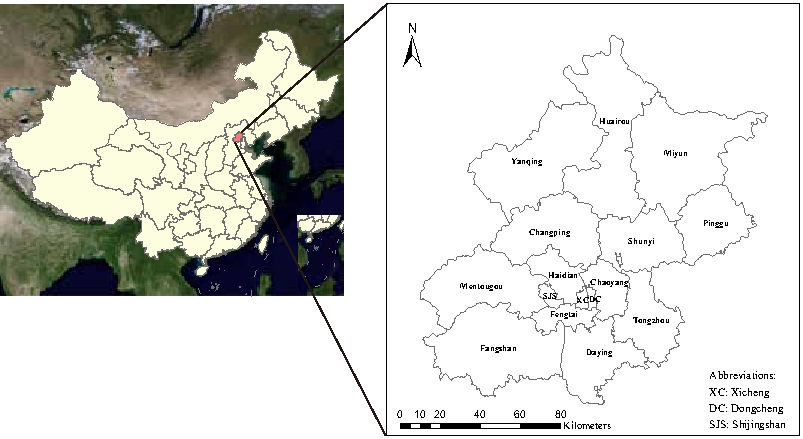
\includegraphics[width=\textwidth]{Figures/StudyArea.pdf}
    \caption{Location map and 16 administrative districts of Beijing}
    \label{fig:study_area}
\end{figure}

\subsection{Study area}
This study is conducted in the city of Beijing, the capital of China. 
As shown in Figure \ref{fig:study_area}, Beijing locates at the North China Plain, occupying an area of 16,411km$^2$ ( 39.4{\degree}-41.6{\degree}N, 115.7{\degree}-117.4{\degree}E). 
In 2019, the municipal population of Beijing have reached 21.53 million. According to Beijing Health Commission, 352 confirmed cases\footnote{\url{http://wjw.beijing.gov.cn/xwzx_20031/wnxw/202002/t20200212_1628835.html} (in Chinese)} were found in Beijing by February 10, 2020. 
As a population-importing metropolis, Beijing has taken measures in response to the outbreak. 
Under this circumstance, the activities of residents have been influenced and showing special spatiotemporal patterns different from ordinary days.

\subsection{Data Sets}
\textbf{BSS spatiotemporal data} Temporal positioning datasets come from 900 thousand share bikes belonging to 3 main BSS operators (Mobike, DiDi Bike, Hellobike and Ofo) in Beijing.
The datasets date from March 2018 to March 2020 (66.8 GB) and cover 1.5 million usages per day contributed by 11 million users which account for one half of the total population of Beijing.
Records of the datasets contain the positioning and timing information of locking \& unlocking bikes, excluding that of rebalancing operations.
This feature suggests that the movement of bikes are done by users.
Certain districts (Chaoyang, Fengtai and Shijingshan) are not comprised in the datasets due to different policies of local governments.

\textbf{The infected residential areas} was collected from the daily update on the novel coronavirus pneumonia outbreak dashboard\footnote{\url{http://wjw.beijing.gov.cn/xwzx_20031/wnxw/202003/t20200305_1679143.html} (as of March 05, 2020, in Chinese)} provided by National Health Commission of the People's Republic of China. 
This data records the confirmed cases of each district from Jan 20 to Mar 5, 2020. 
According to the timeline \cite{li2020early} of the outbreak, we pick several important dates shown in Figure \ref{fig:number_of_confirmed_cases}, visualizing the evolution of the overall situation of Beijing.

\begin{figure}[H]
    \centering
    \begin{subfigure}{.23\textwidth}
        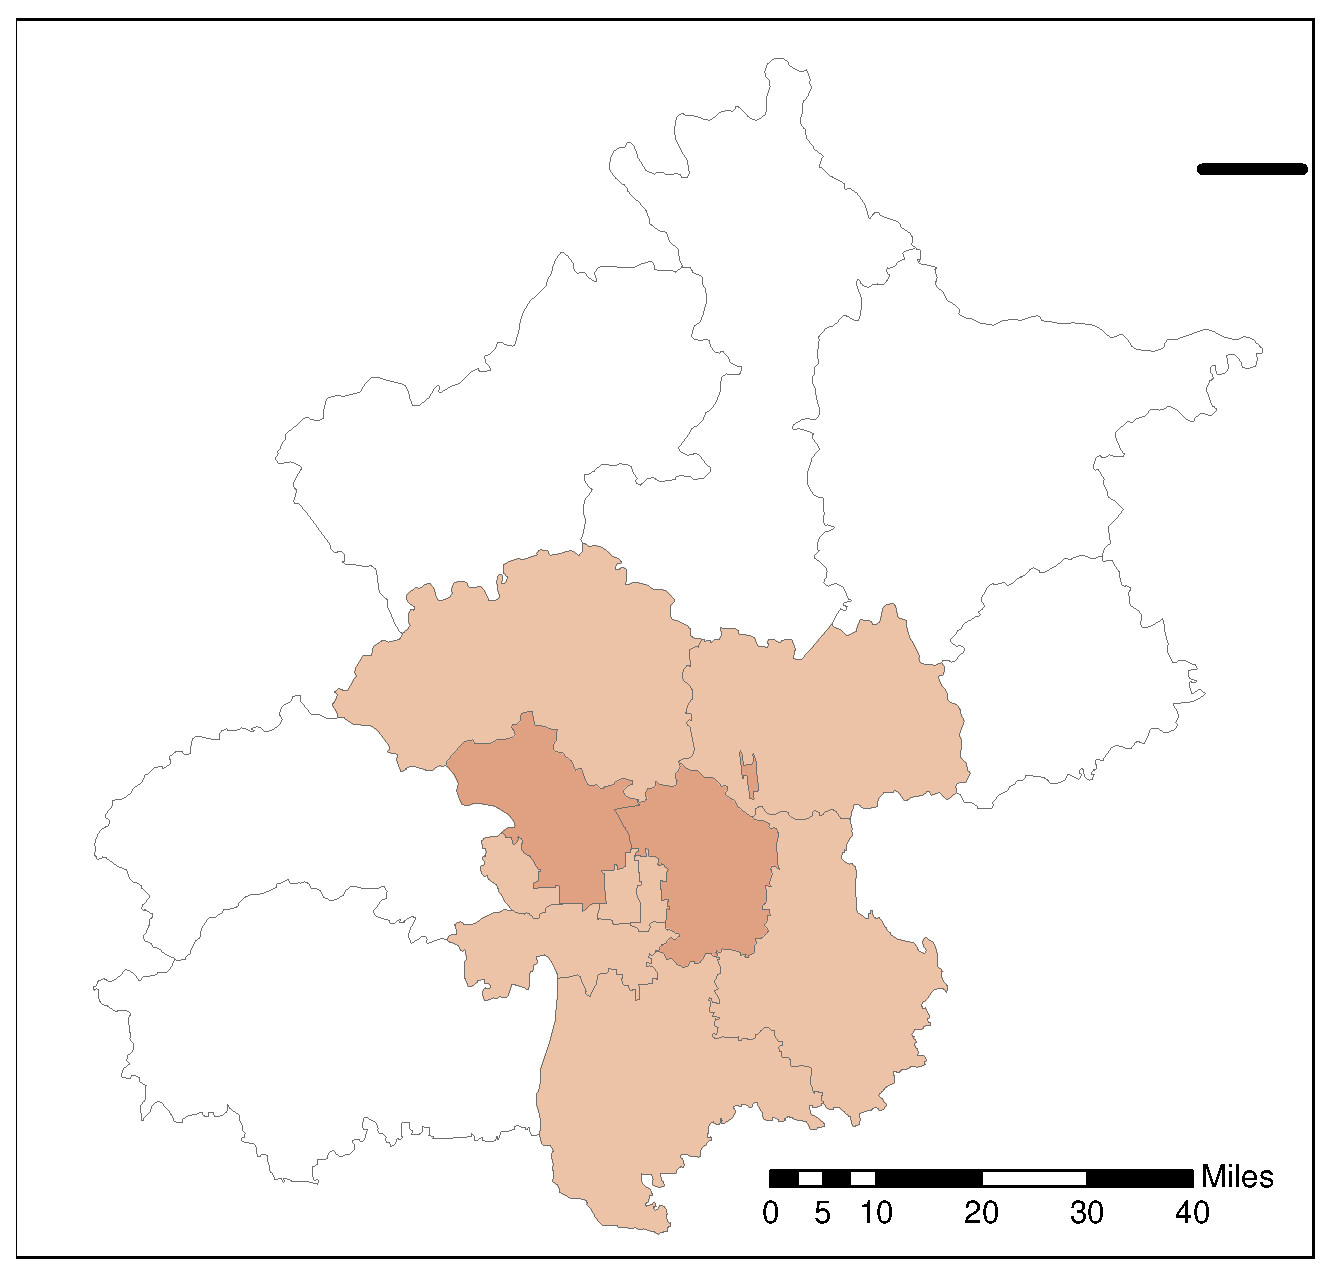
\includegraphics[width=\textwidth]{Figures/ConfirmedDistrictD2020_01_25.eps}
        \caption{25 Jan}
    \end{subfigure}
    \begin{subfigure}{.23\textwidth}
        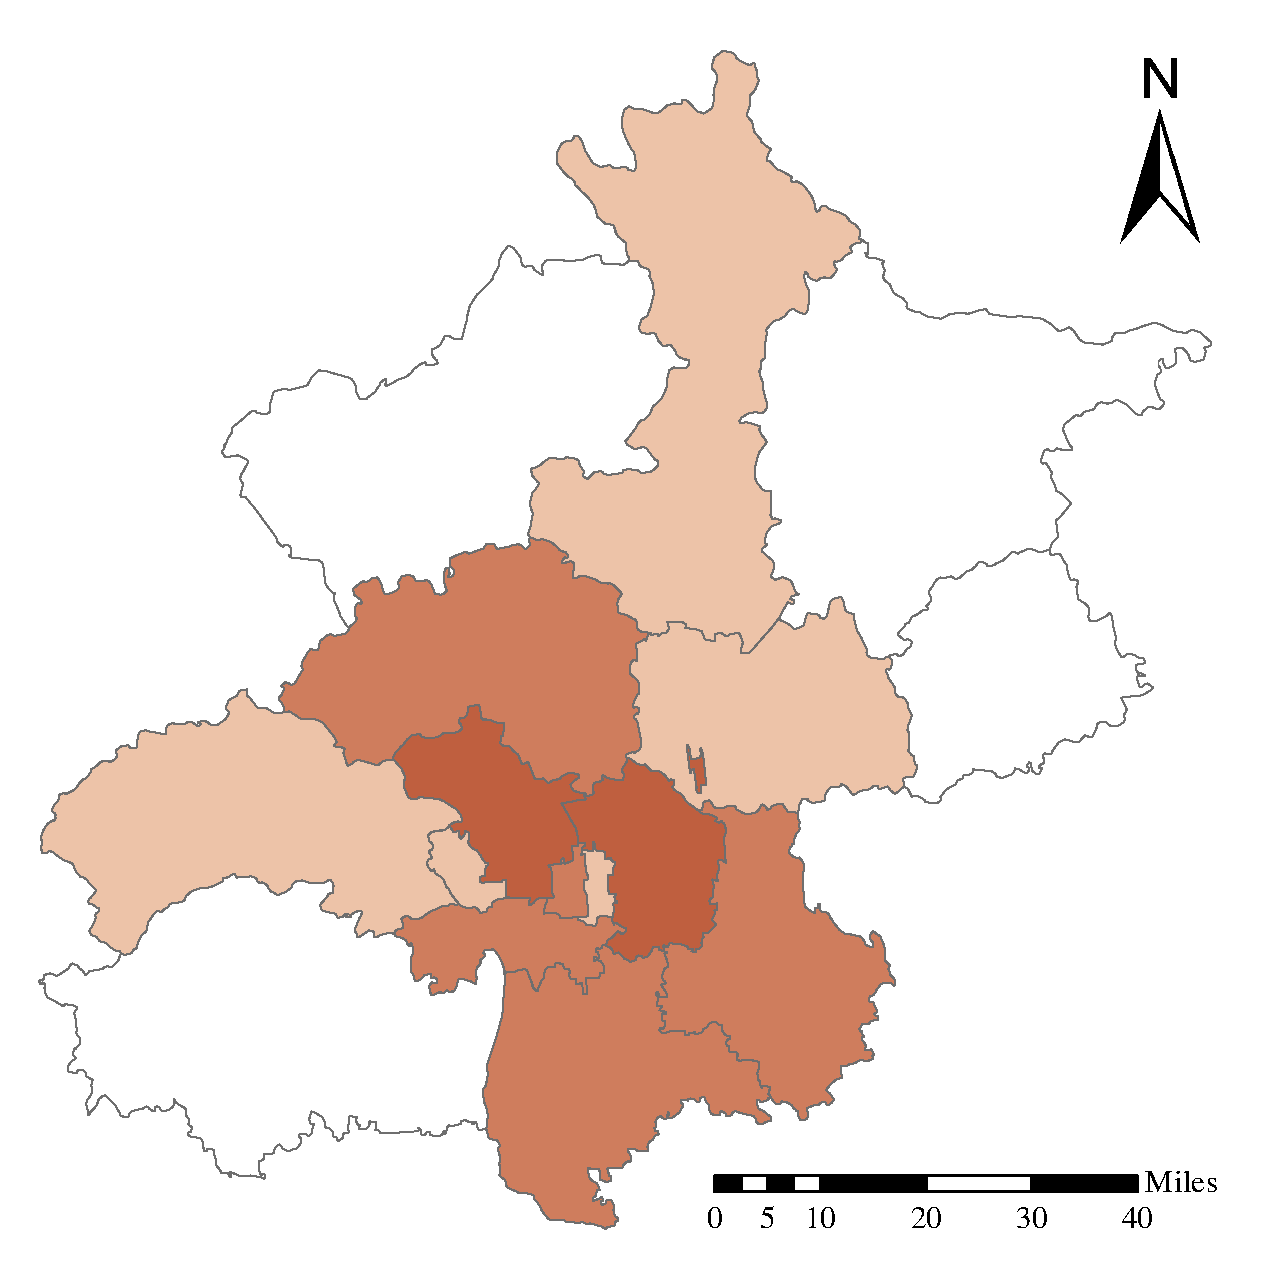
\includegraphics[width=\textwidth]{Figures/ConfirmedDistrictD2020_01_30.eps}
        \caption{30 Jan}
    \end{subfigure}
    \begin{subfigure}{.23\textwidth}
        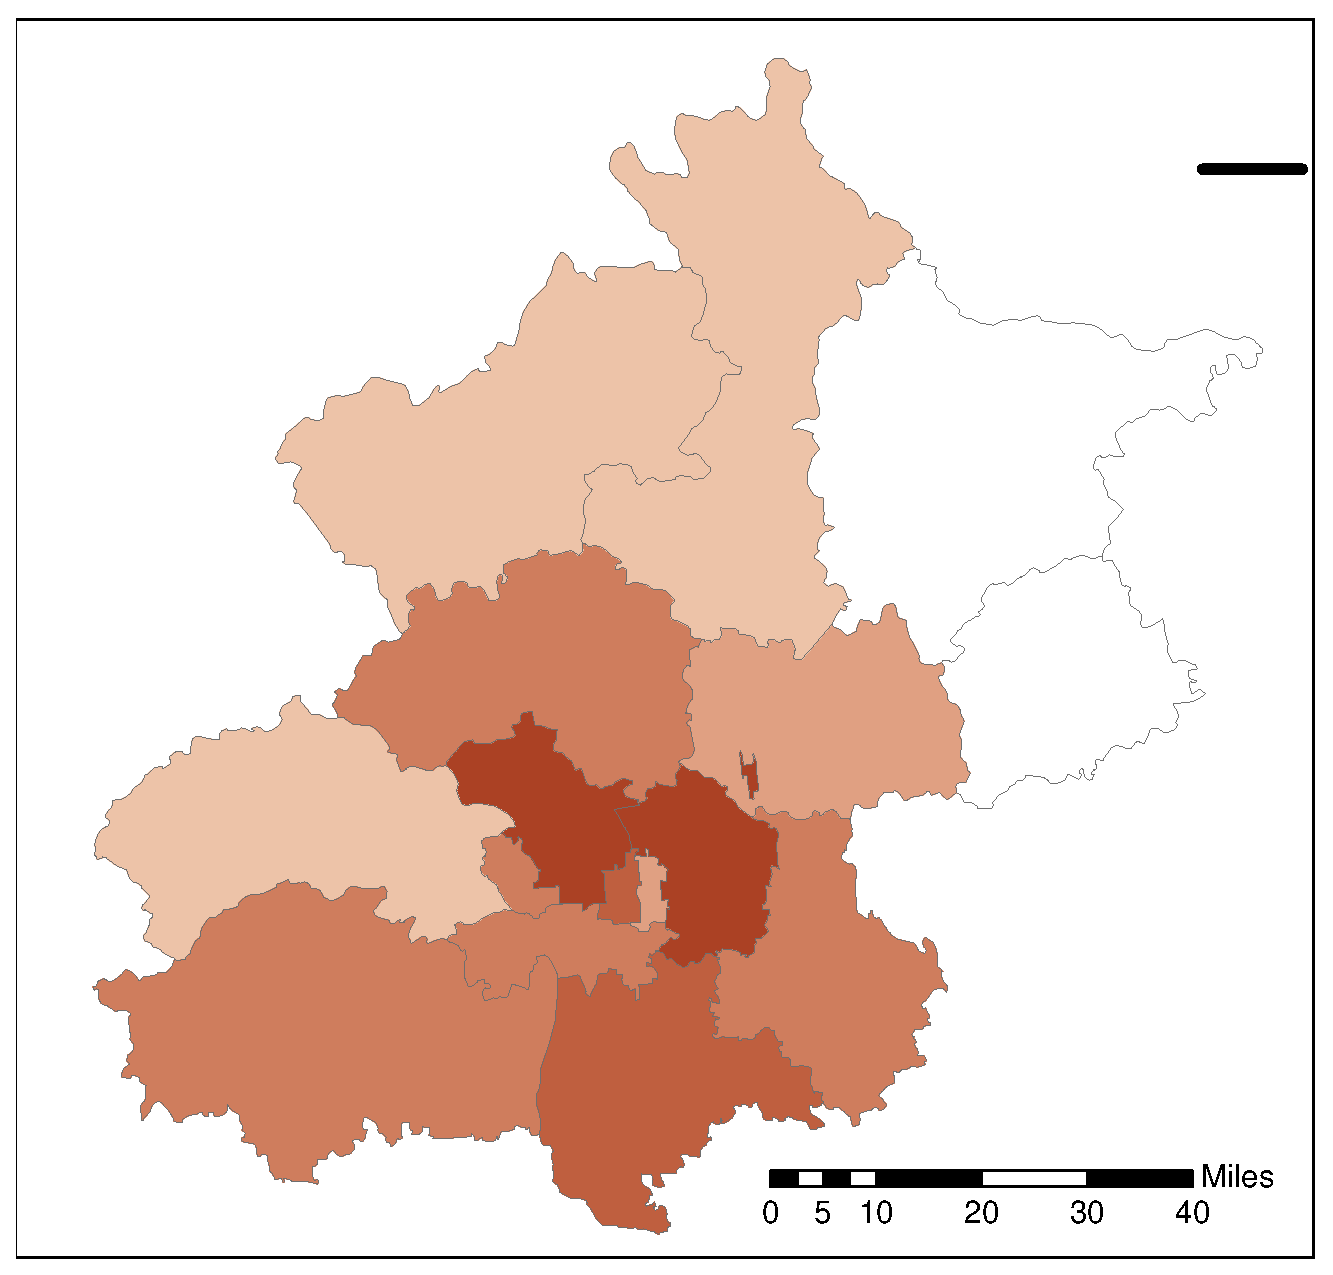
\includegraphics[width=\textwidth]{Figures/ConfirmedDistrictD2020_02_05.eps}
        \caption{05 Feb}
    \end{subfigure}
    \begin{subfigure}{.23\textwidth}
        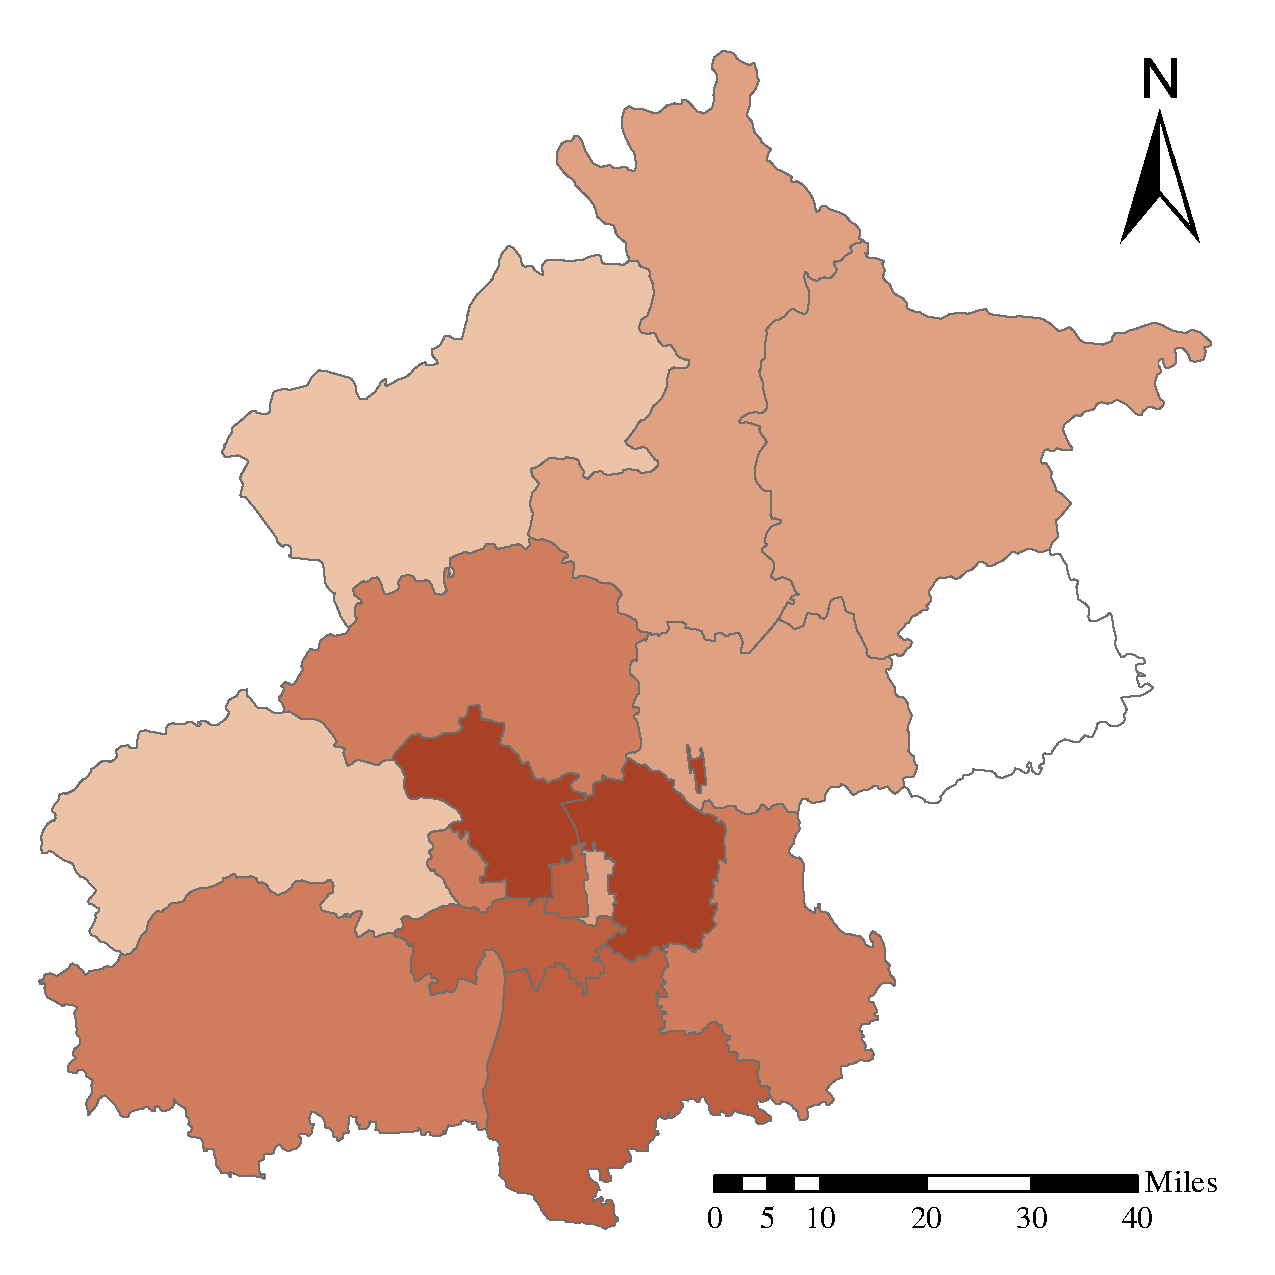
\includegraphics[width=\textwidth]{Figures/ConfirmedDistrictD2020_02_10.eps}
        \caption{10 Feb}
    \end{subfigure}
    \begin{subfigure}{0.7\textwidth}
        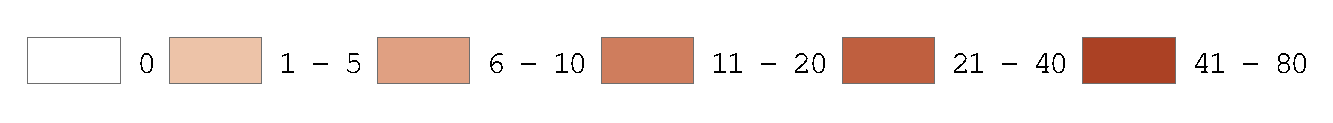
\includegraphics[width=\textwidth]{Figures/Fig2legend.eps}
    \end{subfigure}
    \caption{Number of confirmed cases in Beijing}
    \label{fig:number_of_confirmed_cases}
\end{figure}

\textbf{Points of interests (POIs) data} was collected from AutoNavi API\footnote{\url{https://lbs.amap.com/api/webservice/guide/api/georegeo} (in Chinese)}.
As shown in table \ref{tab:bike_usage} they are classified into seven categories to assess the overall behavior pattern changes.
\textcolor{red}{Explanation to be added when the data are available}

\begin{table}[H]
    \centering
    \begin{tabular}{|l|l|l|}
        \hline
        \multirow{2}{*}{Category} & \multicolumn{2}{c|}{Bike usage}\\
        \cline{2-3}
        & Before the epidemics & During the epidemics\\
        \hline
        Infected communities&&\\
        \hline
        Normal communities&&\\
        \hline
        IT companies&&\\
        \hline
        Other companies&&\\
        \hline
        Metros&&\\
        \hline
        Malls&&\\
        \hline
        Supermarkets&&\\
        \hline
    \end{tabular}
    \caption{Behavior changes before and during the pandemics}
    \label{tab:bike_usage}
\end{table}
By combining the
\begin{figure}[H]
    \centering
    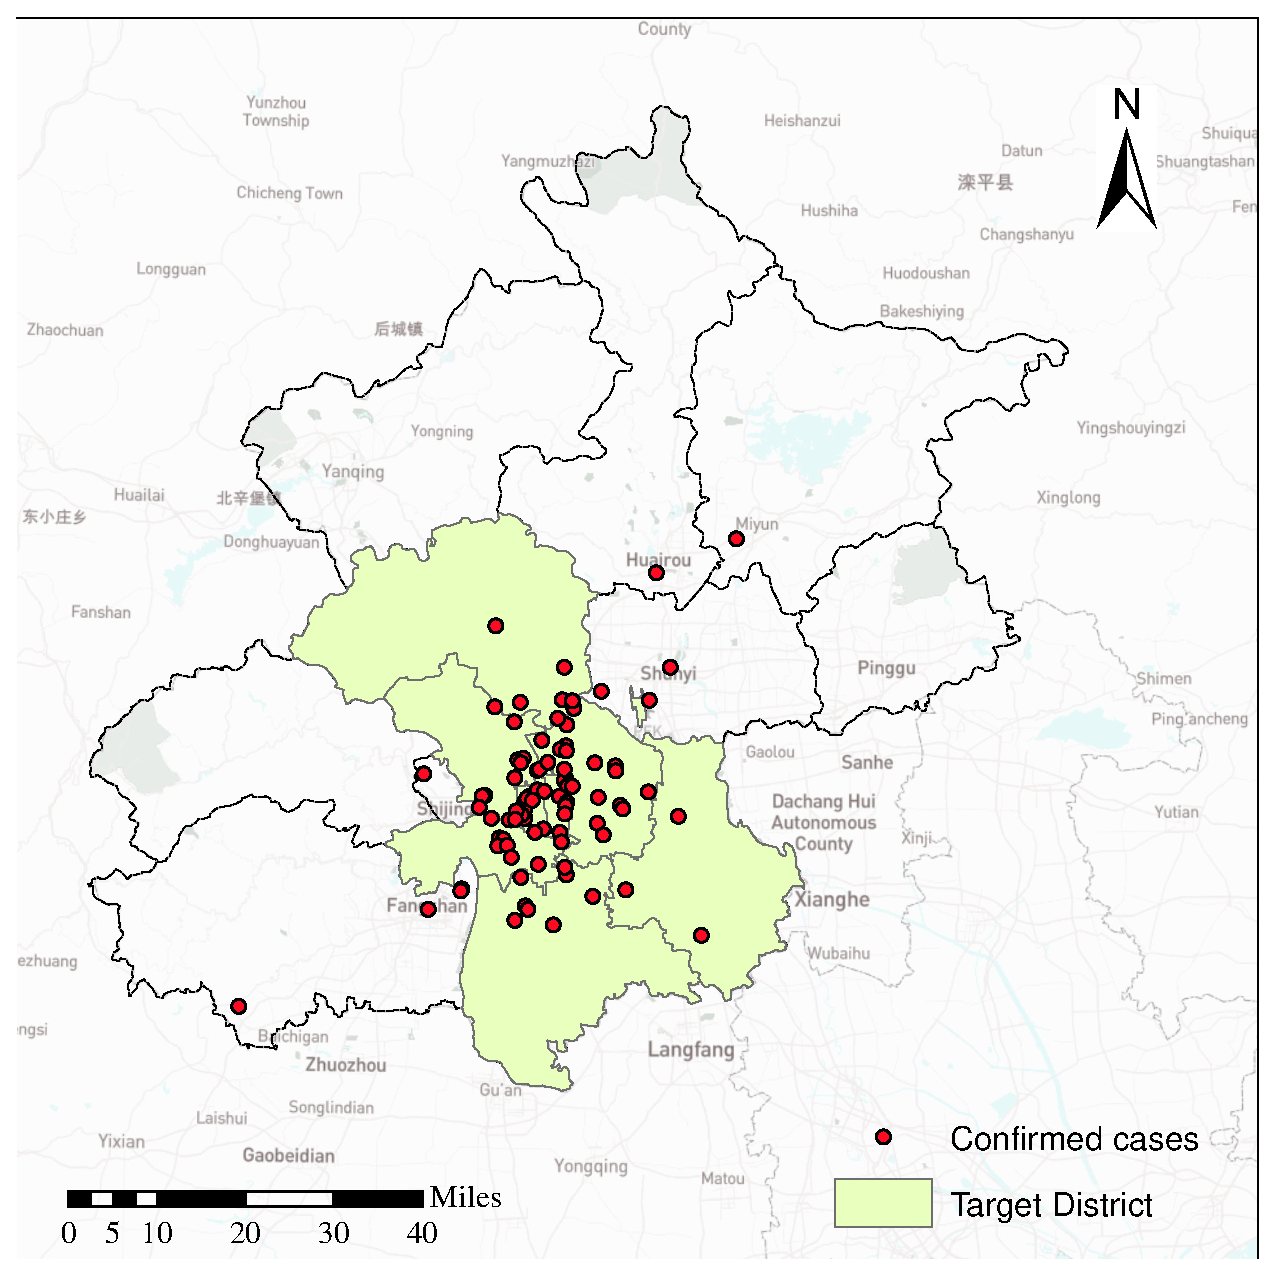
\includegraphics[width=.5\textwidth]{Figures/Plot_location_confirmed_cases.eps}
    \caption{Locations of confirmed cases in Beijing}
    \label{fig:locations_of_confirmed_cases}
\end{figure} 

\subsection{Methods}
To obtain the co-location patterns of huge amount of spatiotemporal data (66.8GB) with numerous POIs, we proceed with GeoSpark SQL \cite{huang2017geospark}, which performs spatial queries via parallel computing on cluster computing framework Spark\footnote{\url{https://spark.apache.org/}}.
Among the spatial queries, we apply \texttt{spatial\_join(geom1, geom2)}, querying if \texttt{geom1} is inside \texttt{geom2} and \texttt{distance\_join(geom1, geom2, dist)} querying if the distance of \texttt{geom1} and \texttt{geom2} is less than \texttt{dist}.

Basic statistics on the evolution over time in different zones of Beijing.\textcolor{red}{explanation GUO} 

\section{Result and Discussion}
\subsection{Temporal patterns of cycling activities}
To characterize the behavior patterns, we select the following important referential dates: 

\begin{table}[H]
    \centering
    \begin{tabular}{ll}
    04 Feb 2019 & Start of Chinese Lunar New Year holiday 2019 \\
    10 Feb 2019 & End of new year holiday 2019\\
    07 Jan 2020 & Identification of COVID-19\\
    22 Jan 2020 & Shut down of Wuhan and other 15 cities\\
    24 Jan 2020 & Start of Chinese Lunar New Year holiday 2020\\
    02 Feb 2020 & End of extended New Year holiday 2020\\
    10 Feb 2020 & Partial restart of social activities
    \end{tabular}
    \caption{Referential dates}
    \label{tab:my_label}
\end{table}


% \begin{figure}[H]
%     \centering
%     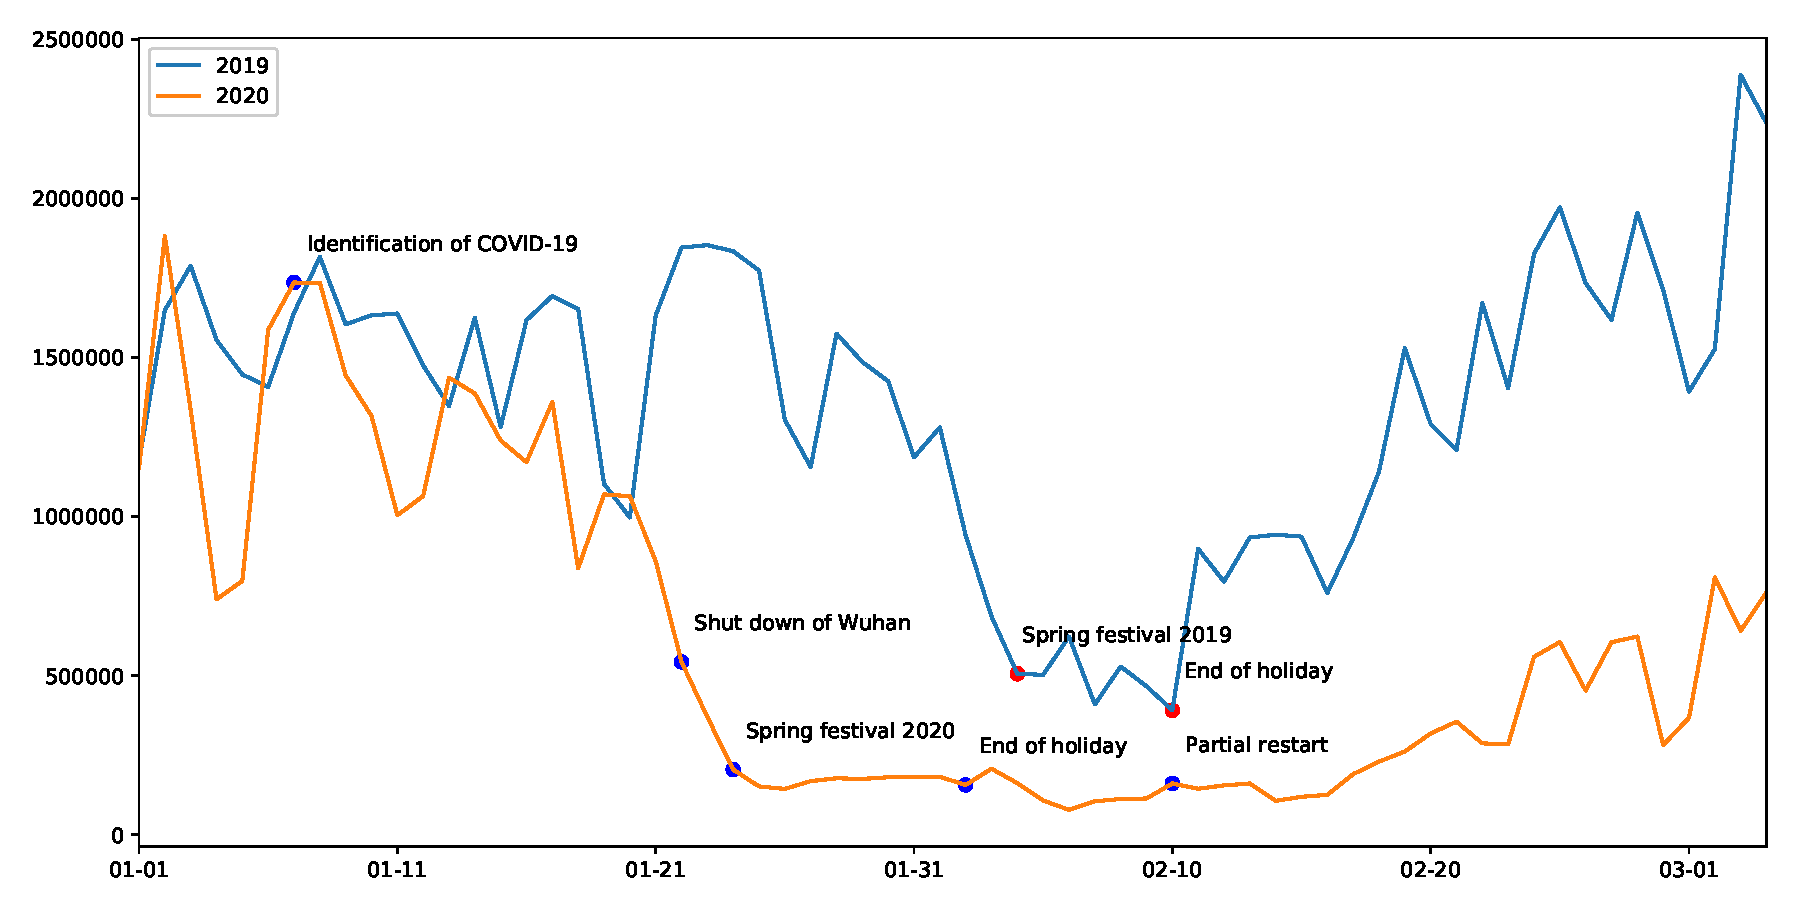
\includegraphics[width=\textwidth]{Compare_temporal.eps}
%     \caption{Comparison between share bike daily usages of year 2019 and 2020.}
%     \label{fig:temporal_comparison}
% \end{figure}

\begin{figure}[H]
    \centering
    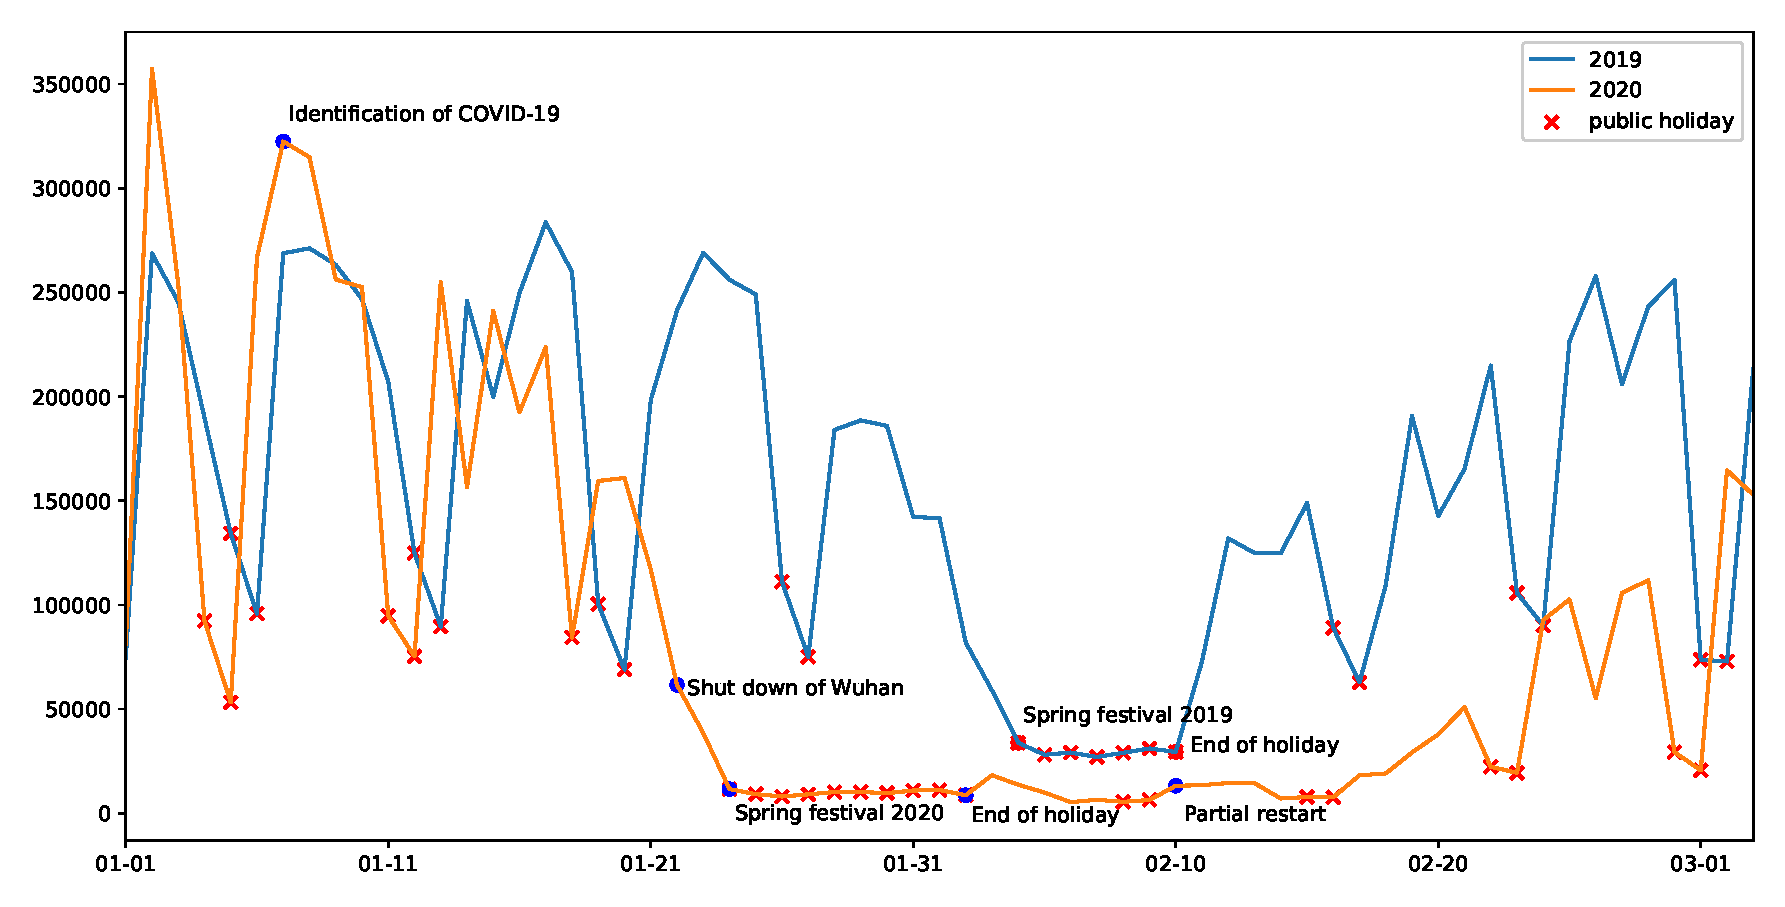
\includegraphics[width=0.9\textwidth]{Figures/hour_8.eps}
    \caption{Share bike usages during 08:00-09:00 of year 2019 and 2020.}
    \label{fig:hour_comparison_8}
\end{figure}

\begin{figure}[H]
    \centering
    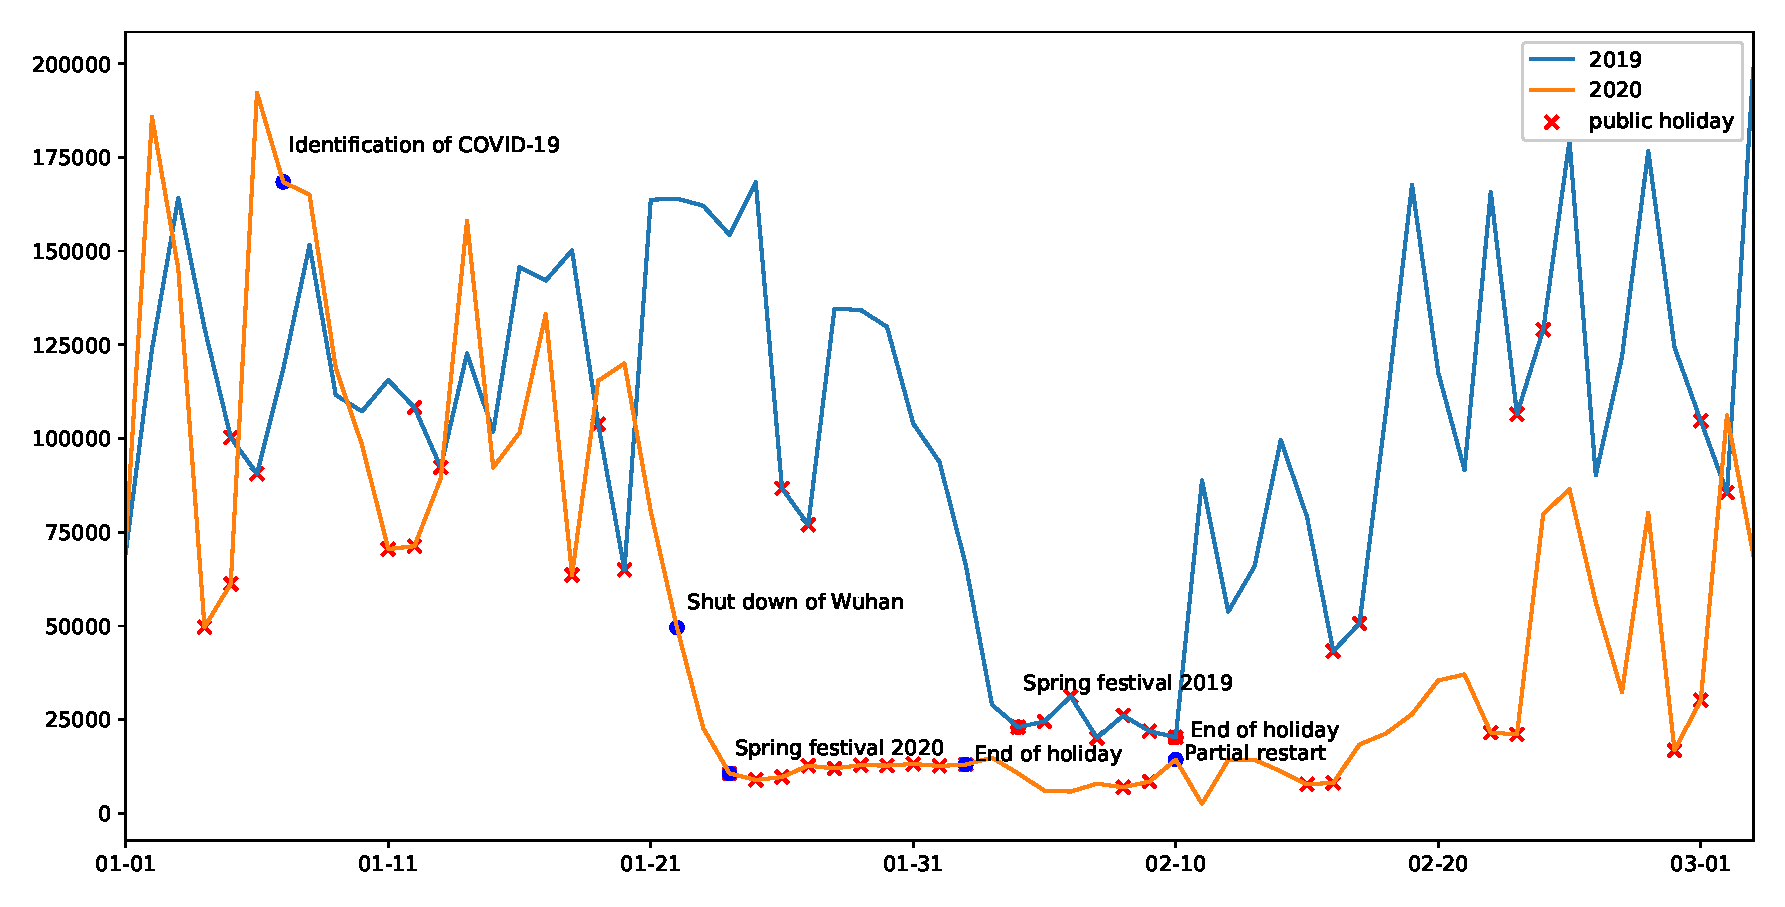
\includegraphics[width=0.9\textwidth]{Figures/hour_18.eps}
    \caption{Share bike usages during 18:00-19:00 of year 2019 and 2020.}
    \label{fig:hour_comparison_18}
\end{figure}

We compared the share bike usage on rush hours (8:00-09:00 and 18:00-19:00) during a period of 64 days from 01 Jan to 05 March 2019 and 01 Jan to 04 March 2020 respectively (data later than 29 Feb 2020 were delayed by one day due to the leap year).
% As can be seen in Figure \ref{fig:temporal_comparison}, in 2019, the usage drops down to $5\times 10^5$ because of spring festival; 
% while in 2020, the usage decreases even two thirds of that in 2019 due to the outbreak of COVID-19 and the following epidemics.

% We also plotted the graph of share bike usage during rush hour (8:00-10:00 and 18:00-20:00) which reflects the industrial activities.
Share bike usage on rush hours in 2019 exhibits the periodicity of social activities: high on weekdays and low on weekends, which fits our general knowledge.
However, this pattern does not appear from 10 Feb 2020 when the government declared the partial restart of certain social activities.
We suggest that the social activities were not resumed until Feb 24, which correspond the impact of epidemics still lasted till the end of the study period.

\subsection{Spatiotemporal patterns of cycling activities\textbf{[Guo]}}

\textcolor{red}{Overall spatial patterns of cycling activities from 21 Jan to 02 Mar.}

\begin{figure}[H]
    \centering
    \begin{subfigure}{.23\textwidth}
        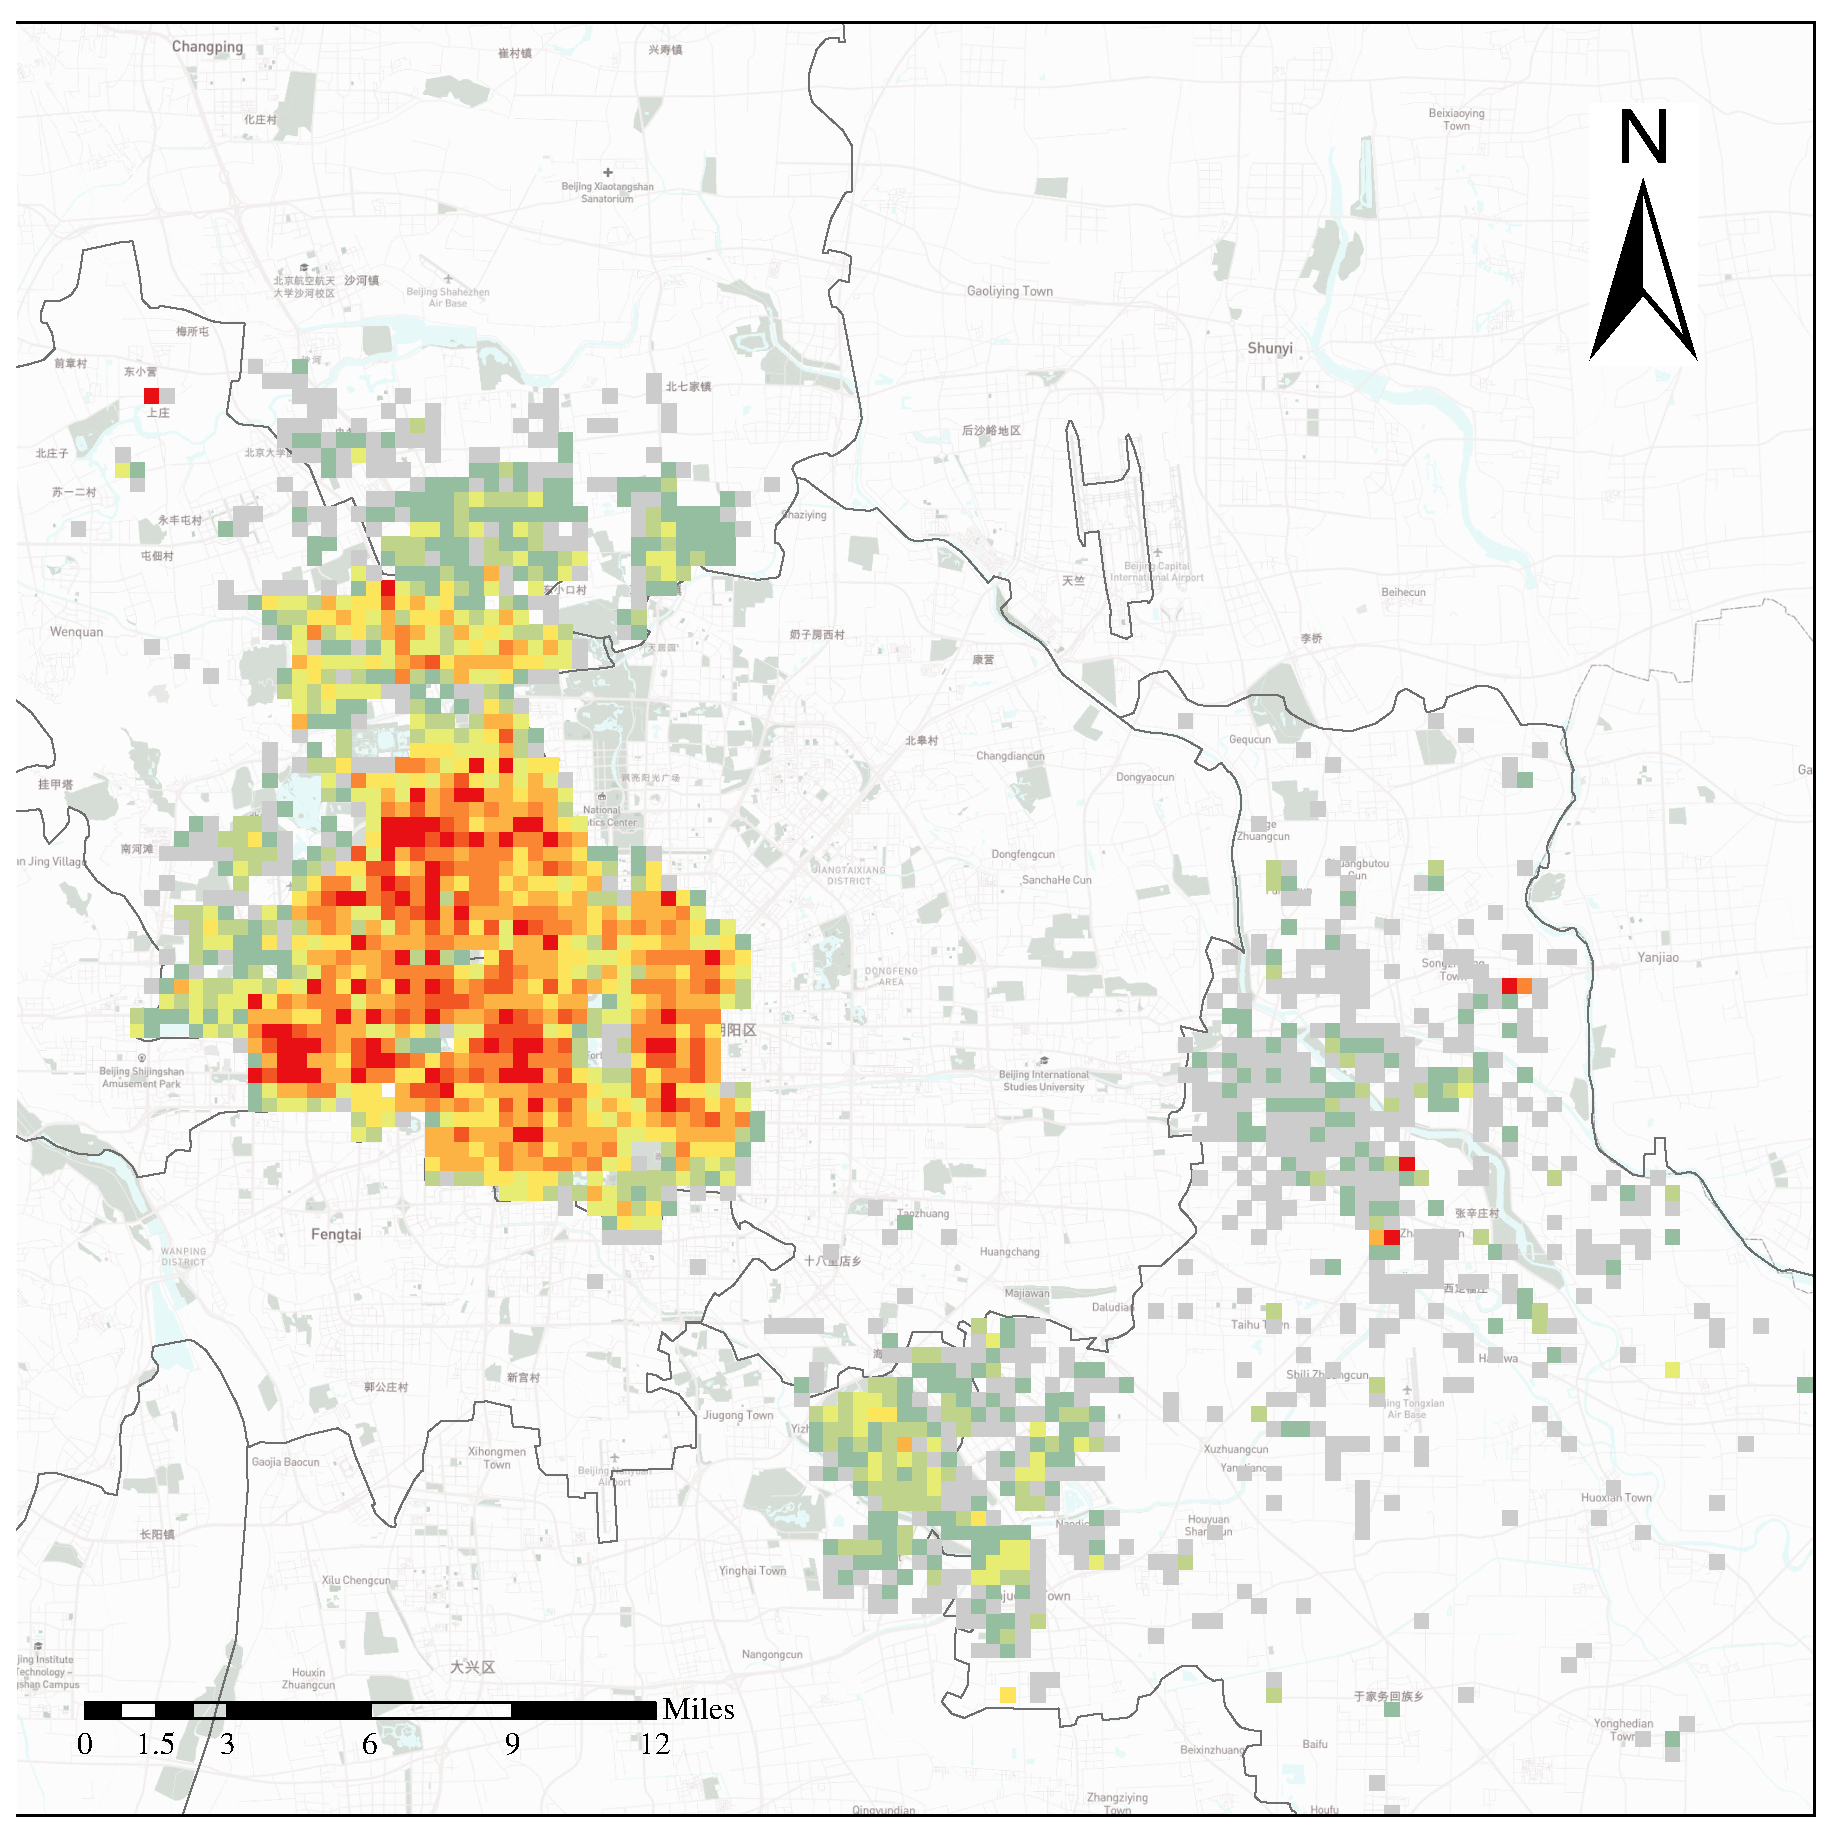
\includegraphics[width=\textwidth]{Figures/Overall_spatial_patterns/FN5_D2020_01_21.eps}
        \caption{21 Jan}
    \end{subfigure}
    \begin{subfigure}{.23\textwidth}
        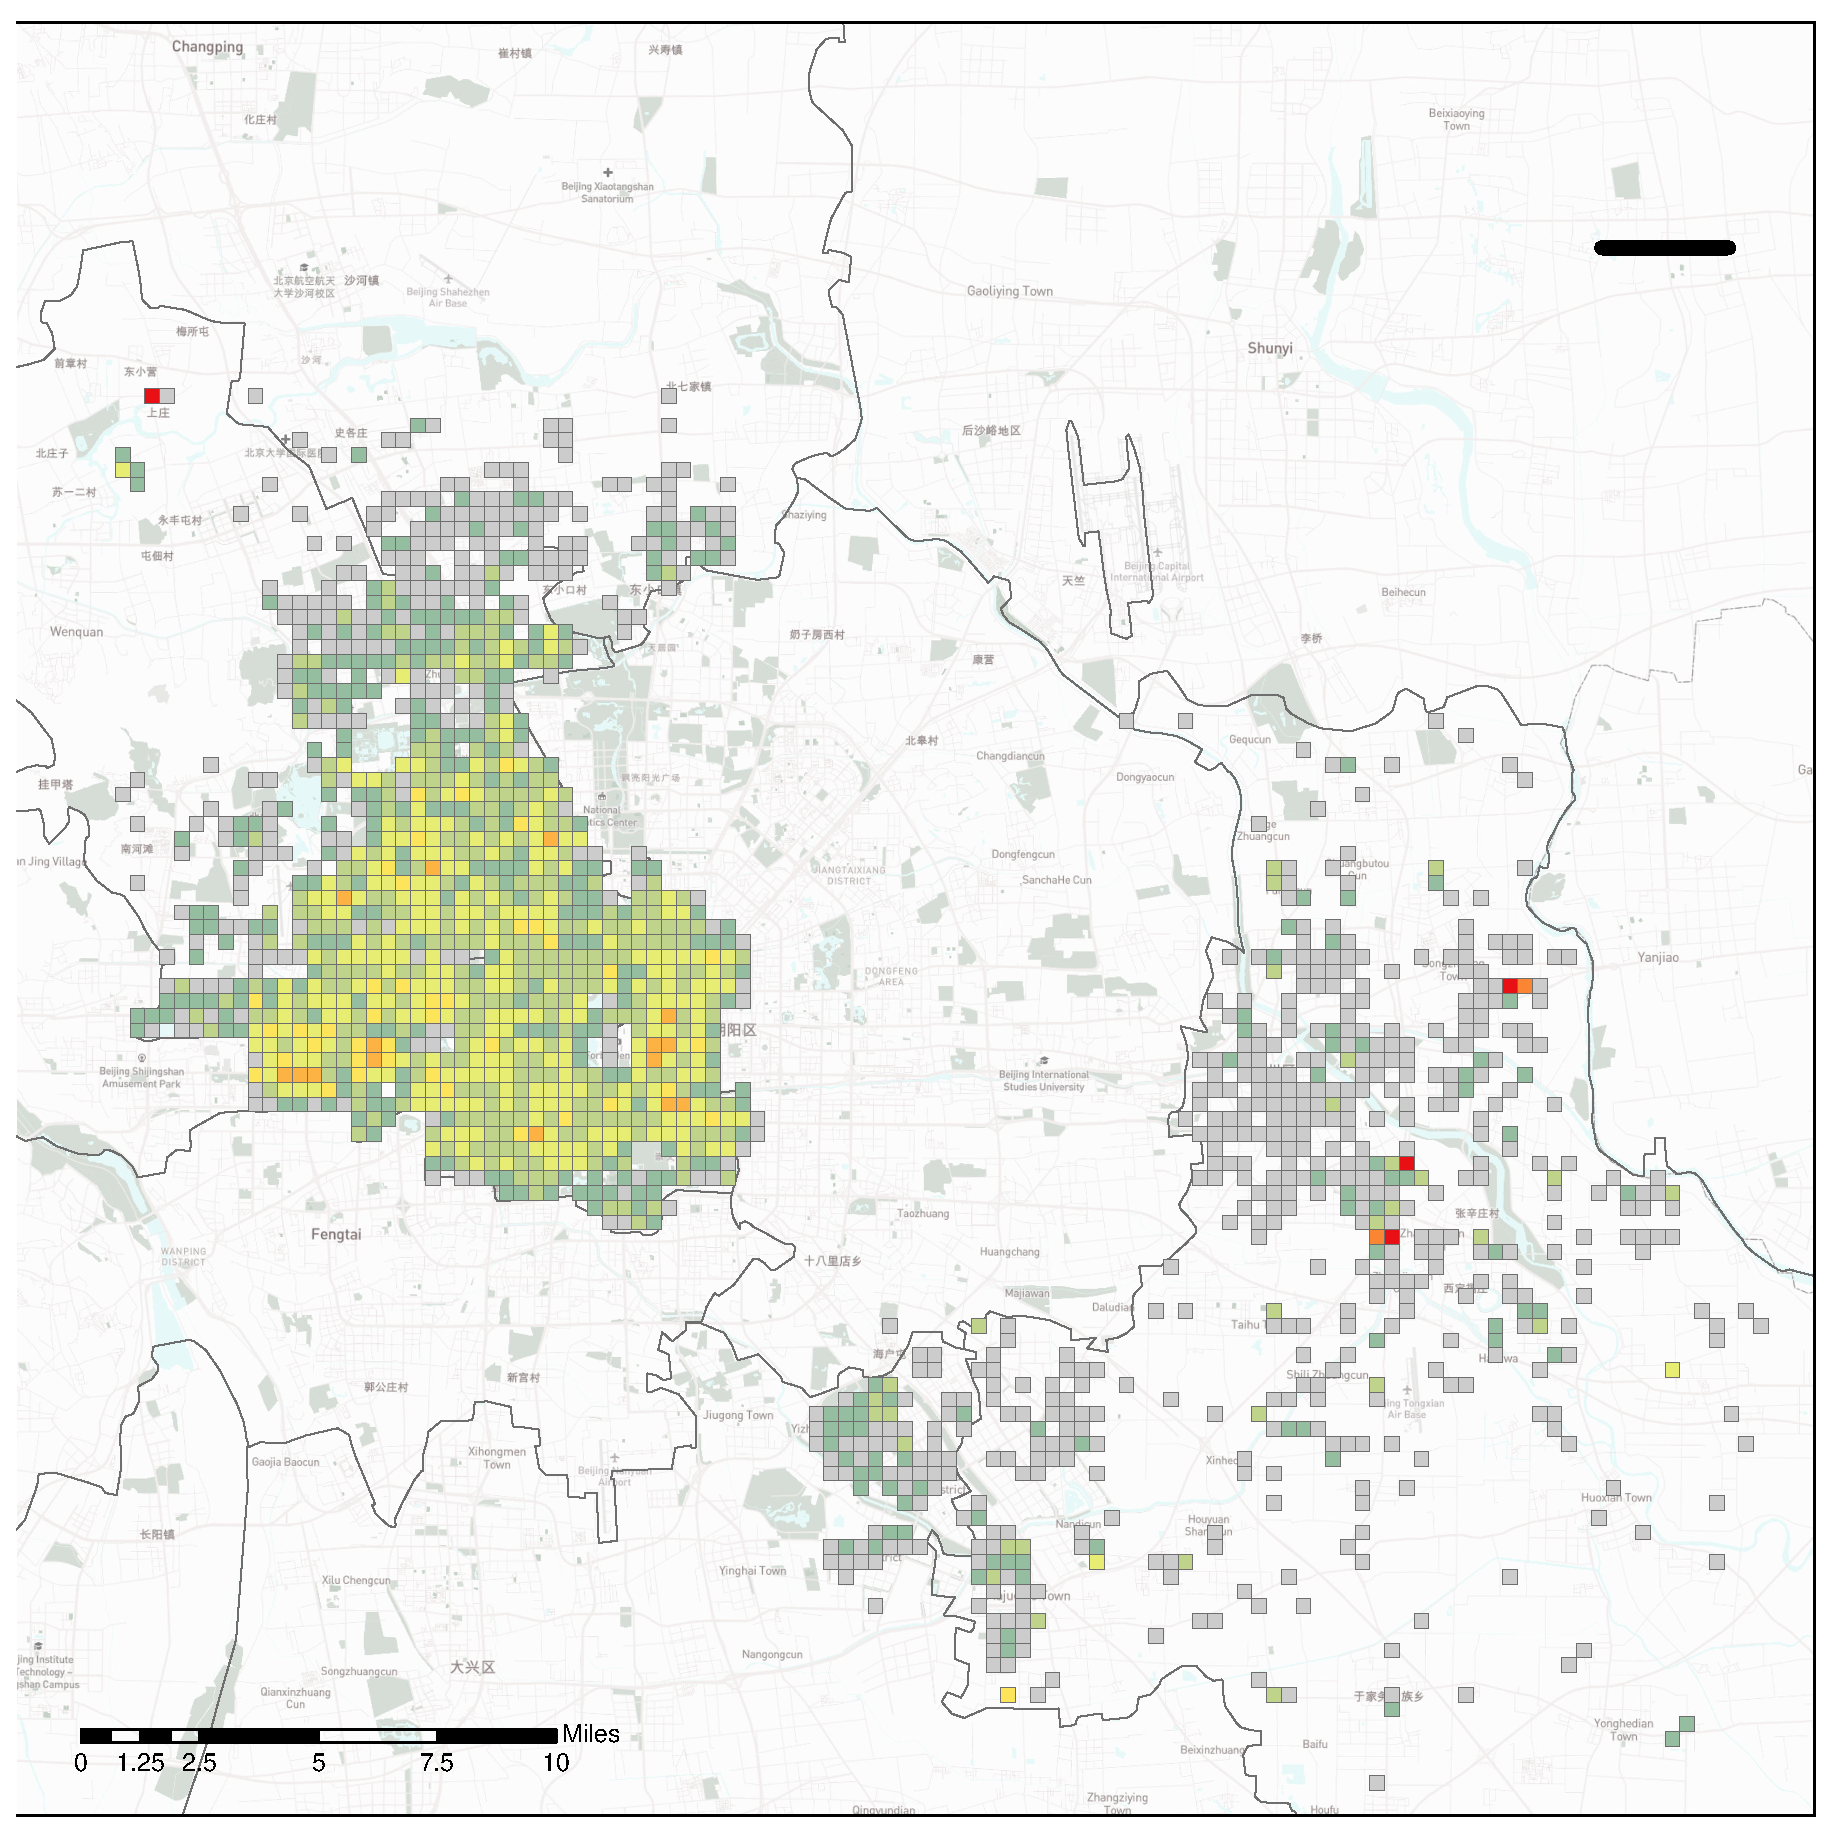
\includegraphics[width=\textwidth]{Figures/Overall_spatial_patterns/FN5_D2020_01_25.eps}
        \caption{25 Jan}
    \end{subfigure}
    \begin{subfigure}{.23\textwidth}
        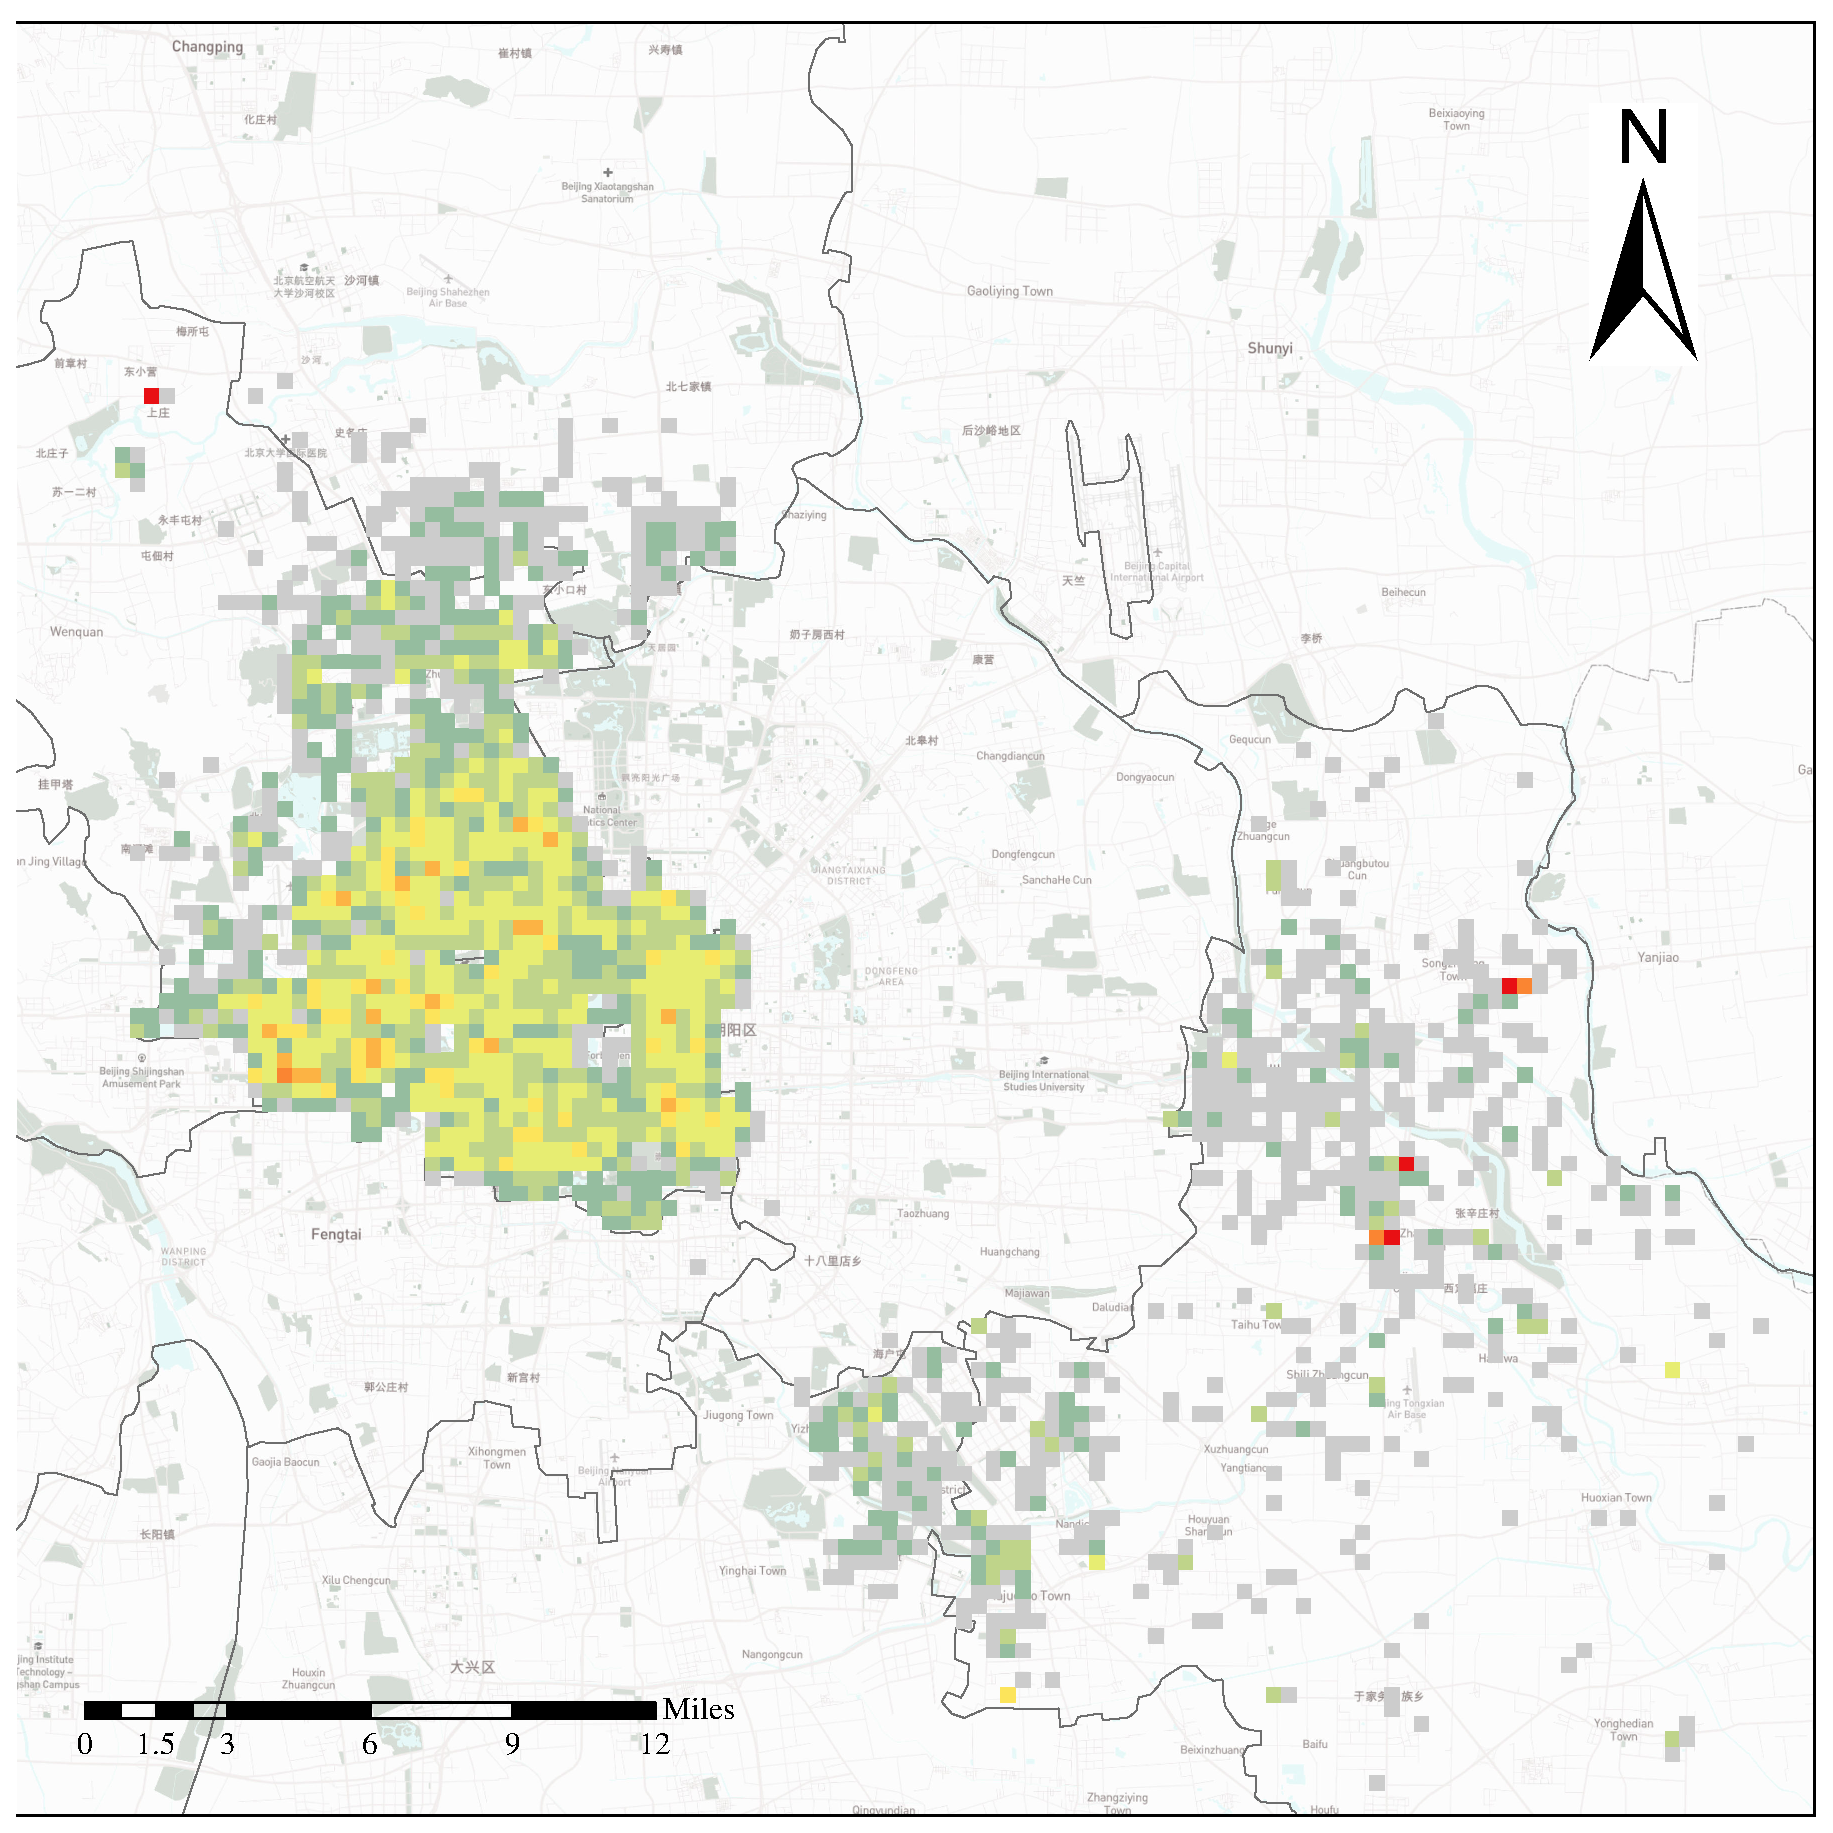
\includegraphics[width=\textwidth]{Figures/Overall_spatial_patterns/FN5_D2020_01_29.eps}
        \caption{29 Jan}
    \end{subfigure}
        \begin{subfigure}{.23\textwidth}
        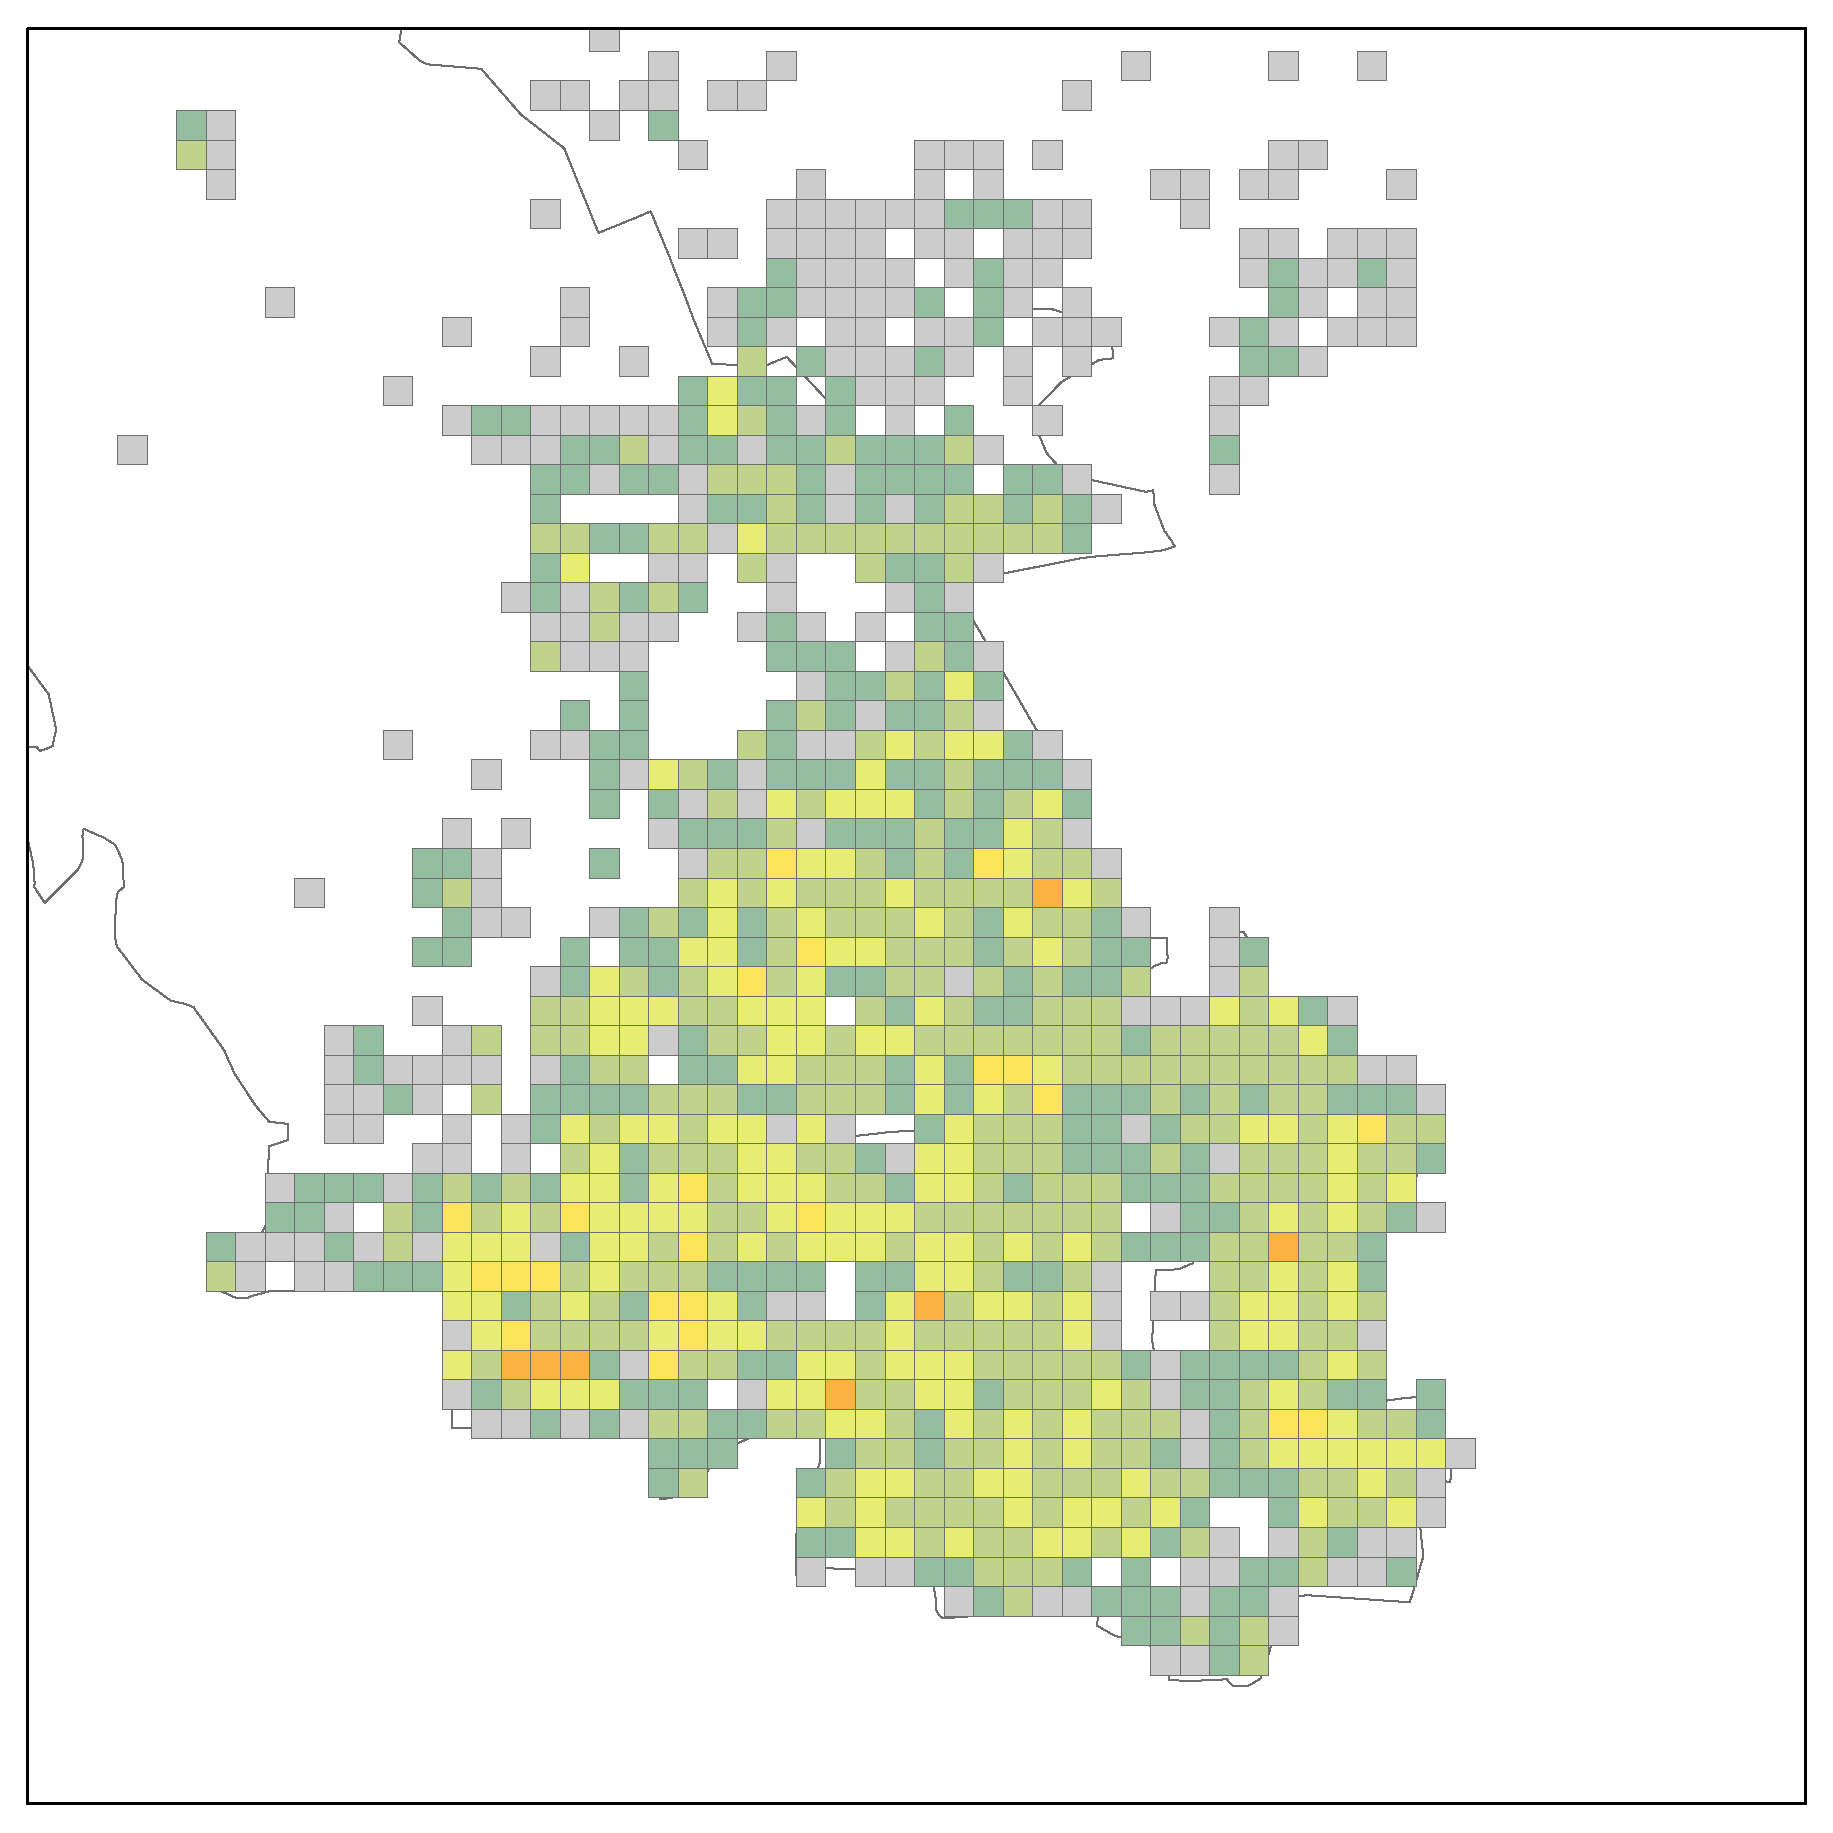
\includegraphics[width=\textwidth]{Figures/Overall_spatial_patterns/FN5_D2020_02_02.eps}
        \caption{02 Feb}
    \end{subfigure}
    
    \vspace{6pt}
    \begin{subfigure}{.23\textwidth}
        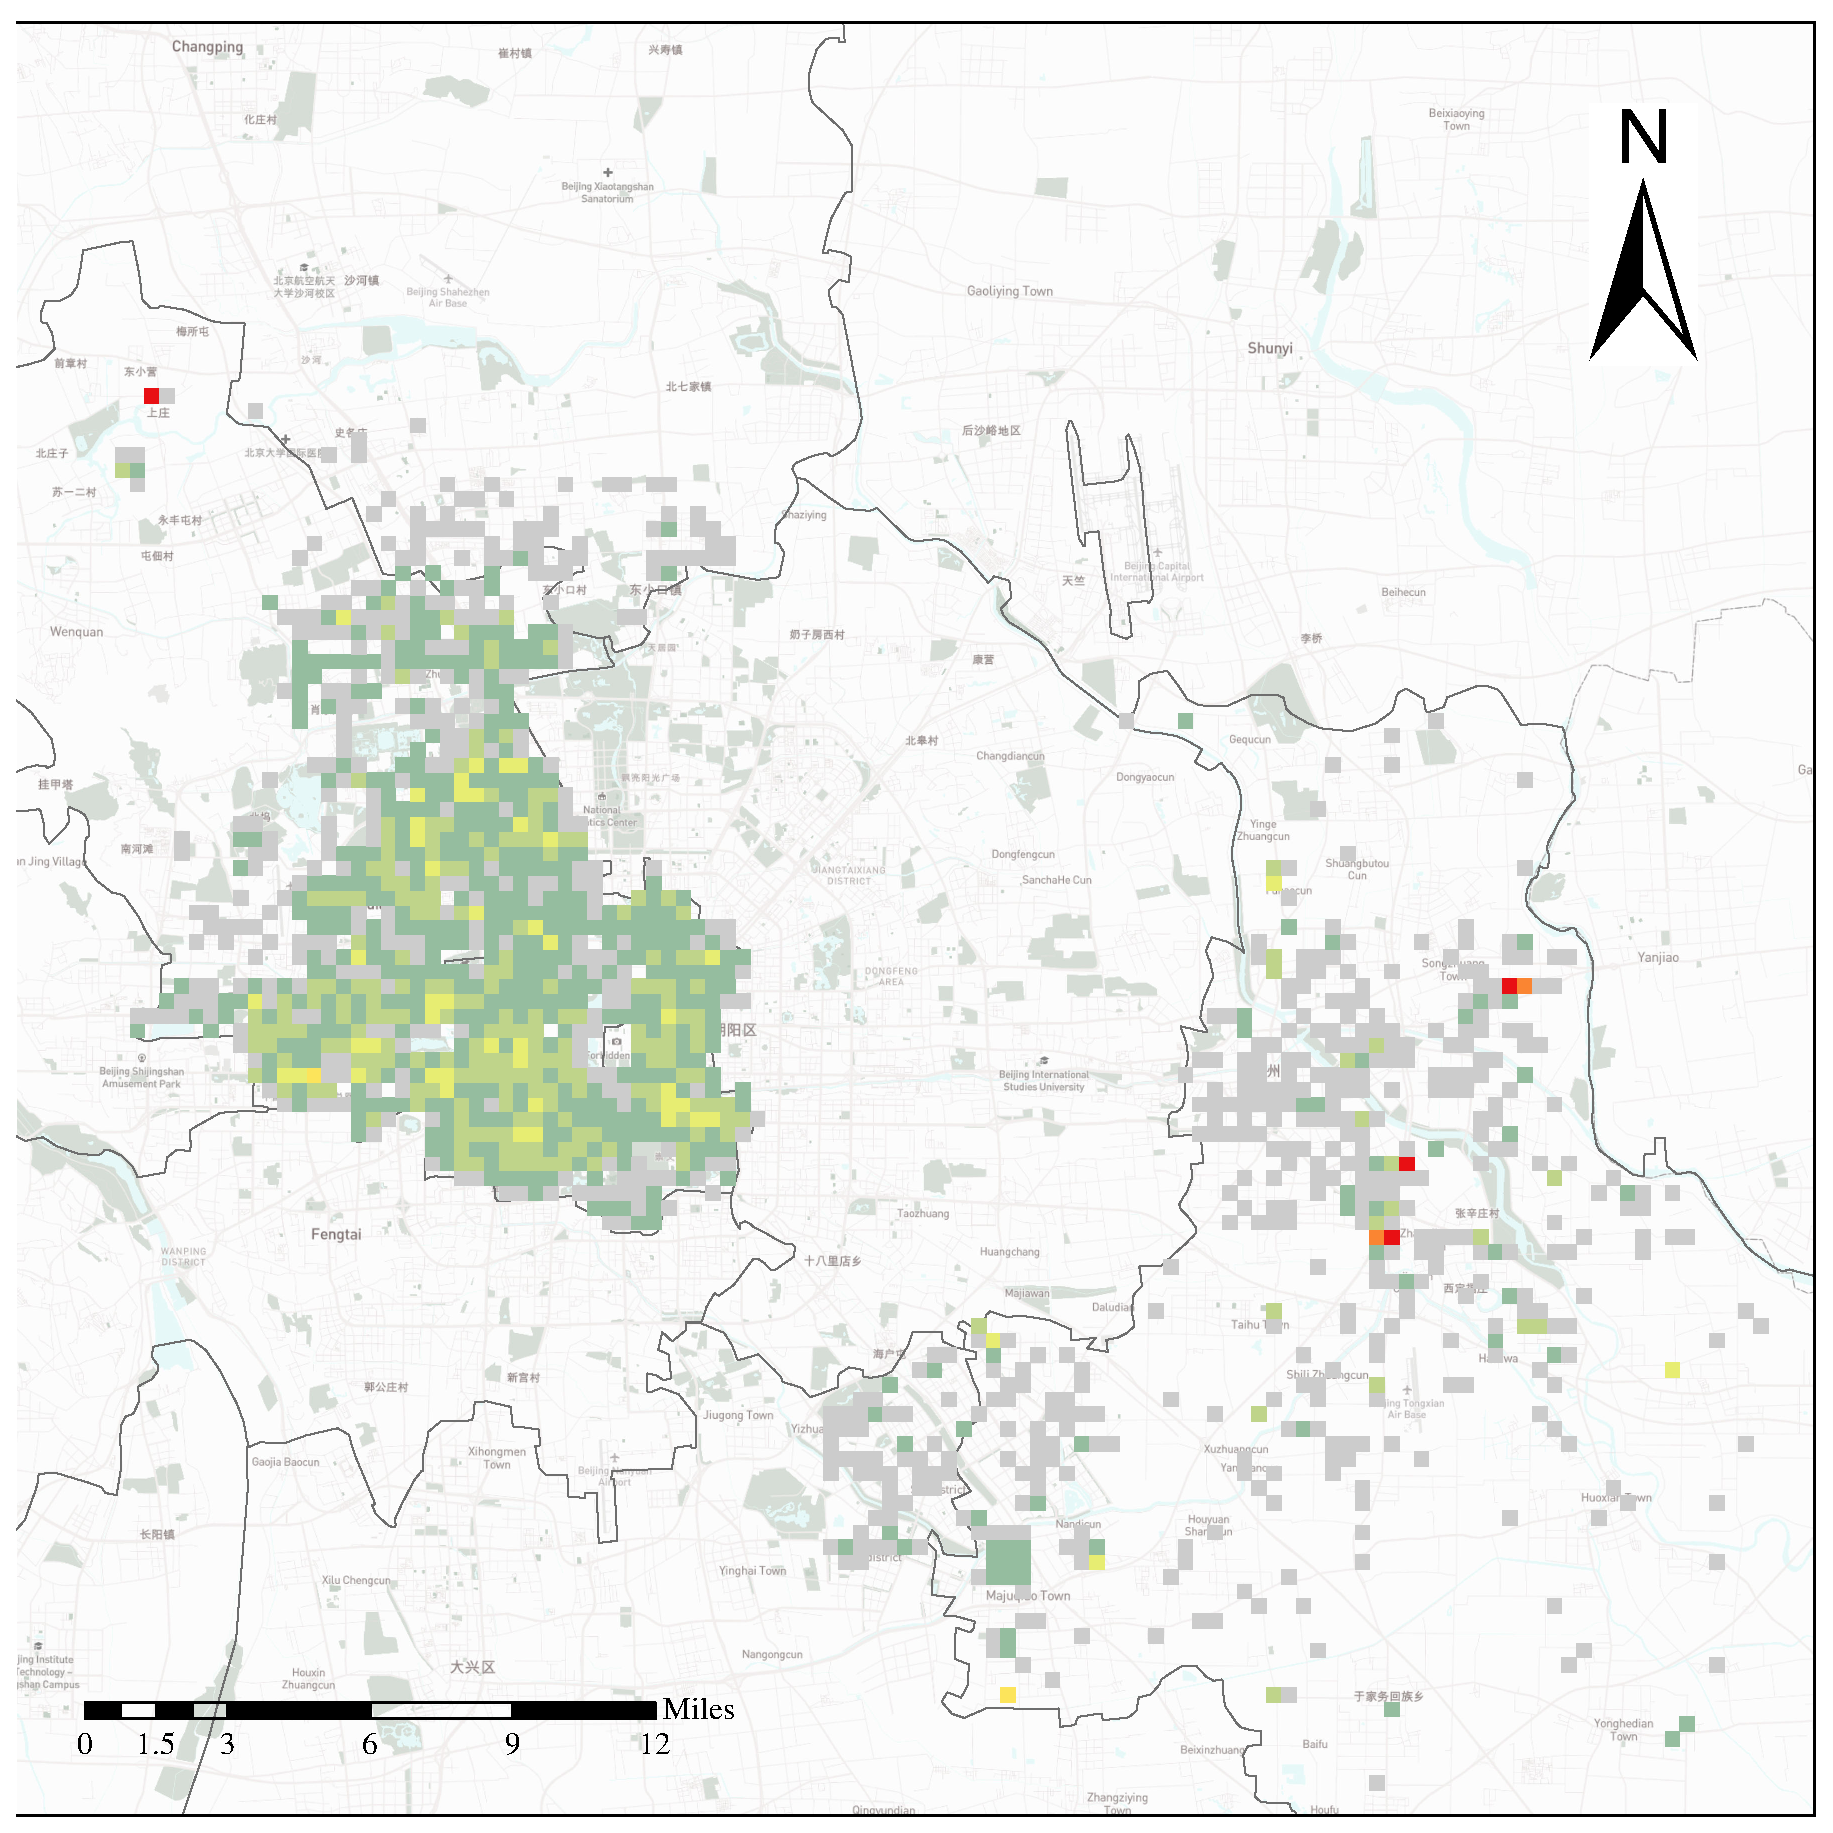
\includegraphics[width=\textwidth]{Figures/Overall_spatial_patterns/FN5_D2020_02_06.eps}
        \caption{06 Feb}
    \end{subfigure}
    \begin{subfigure}{.23\textwidth}
        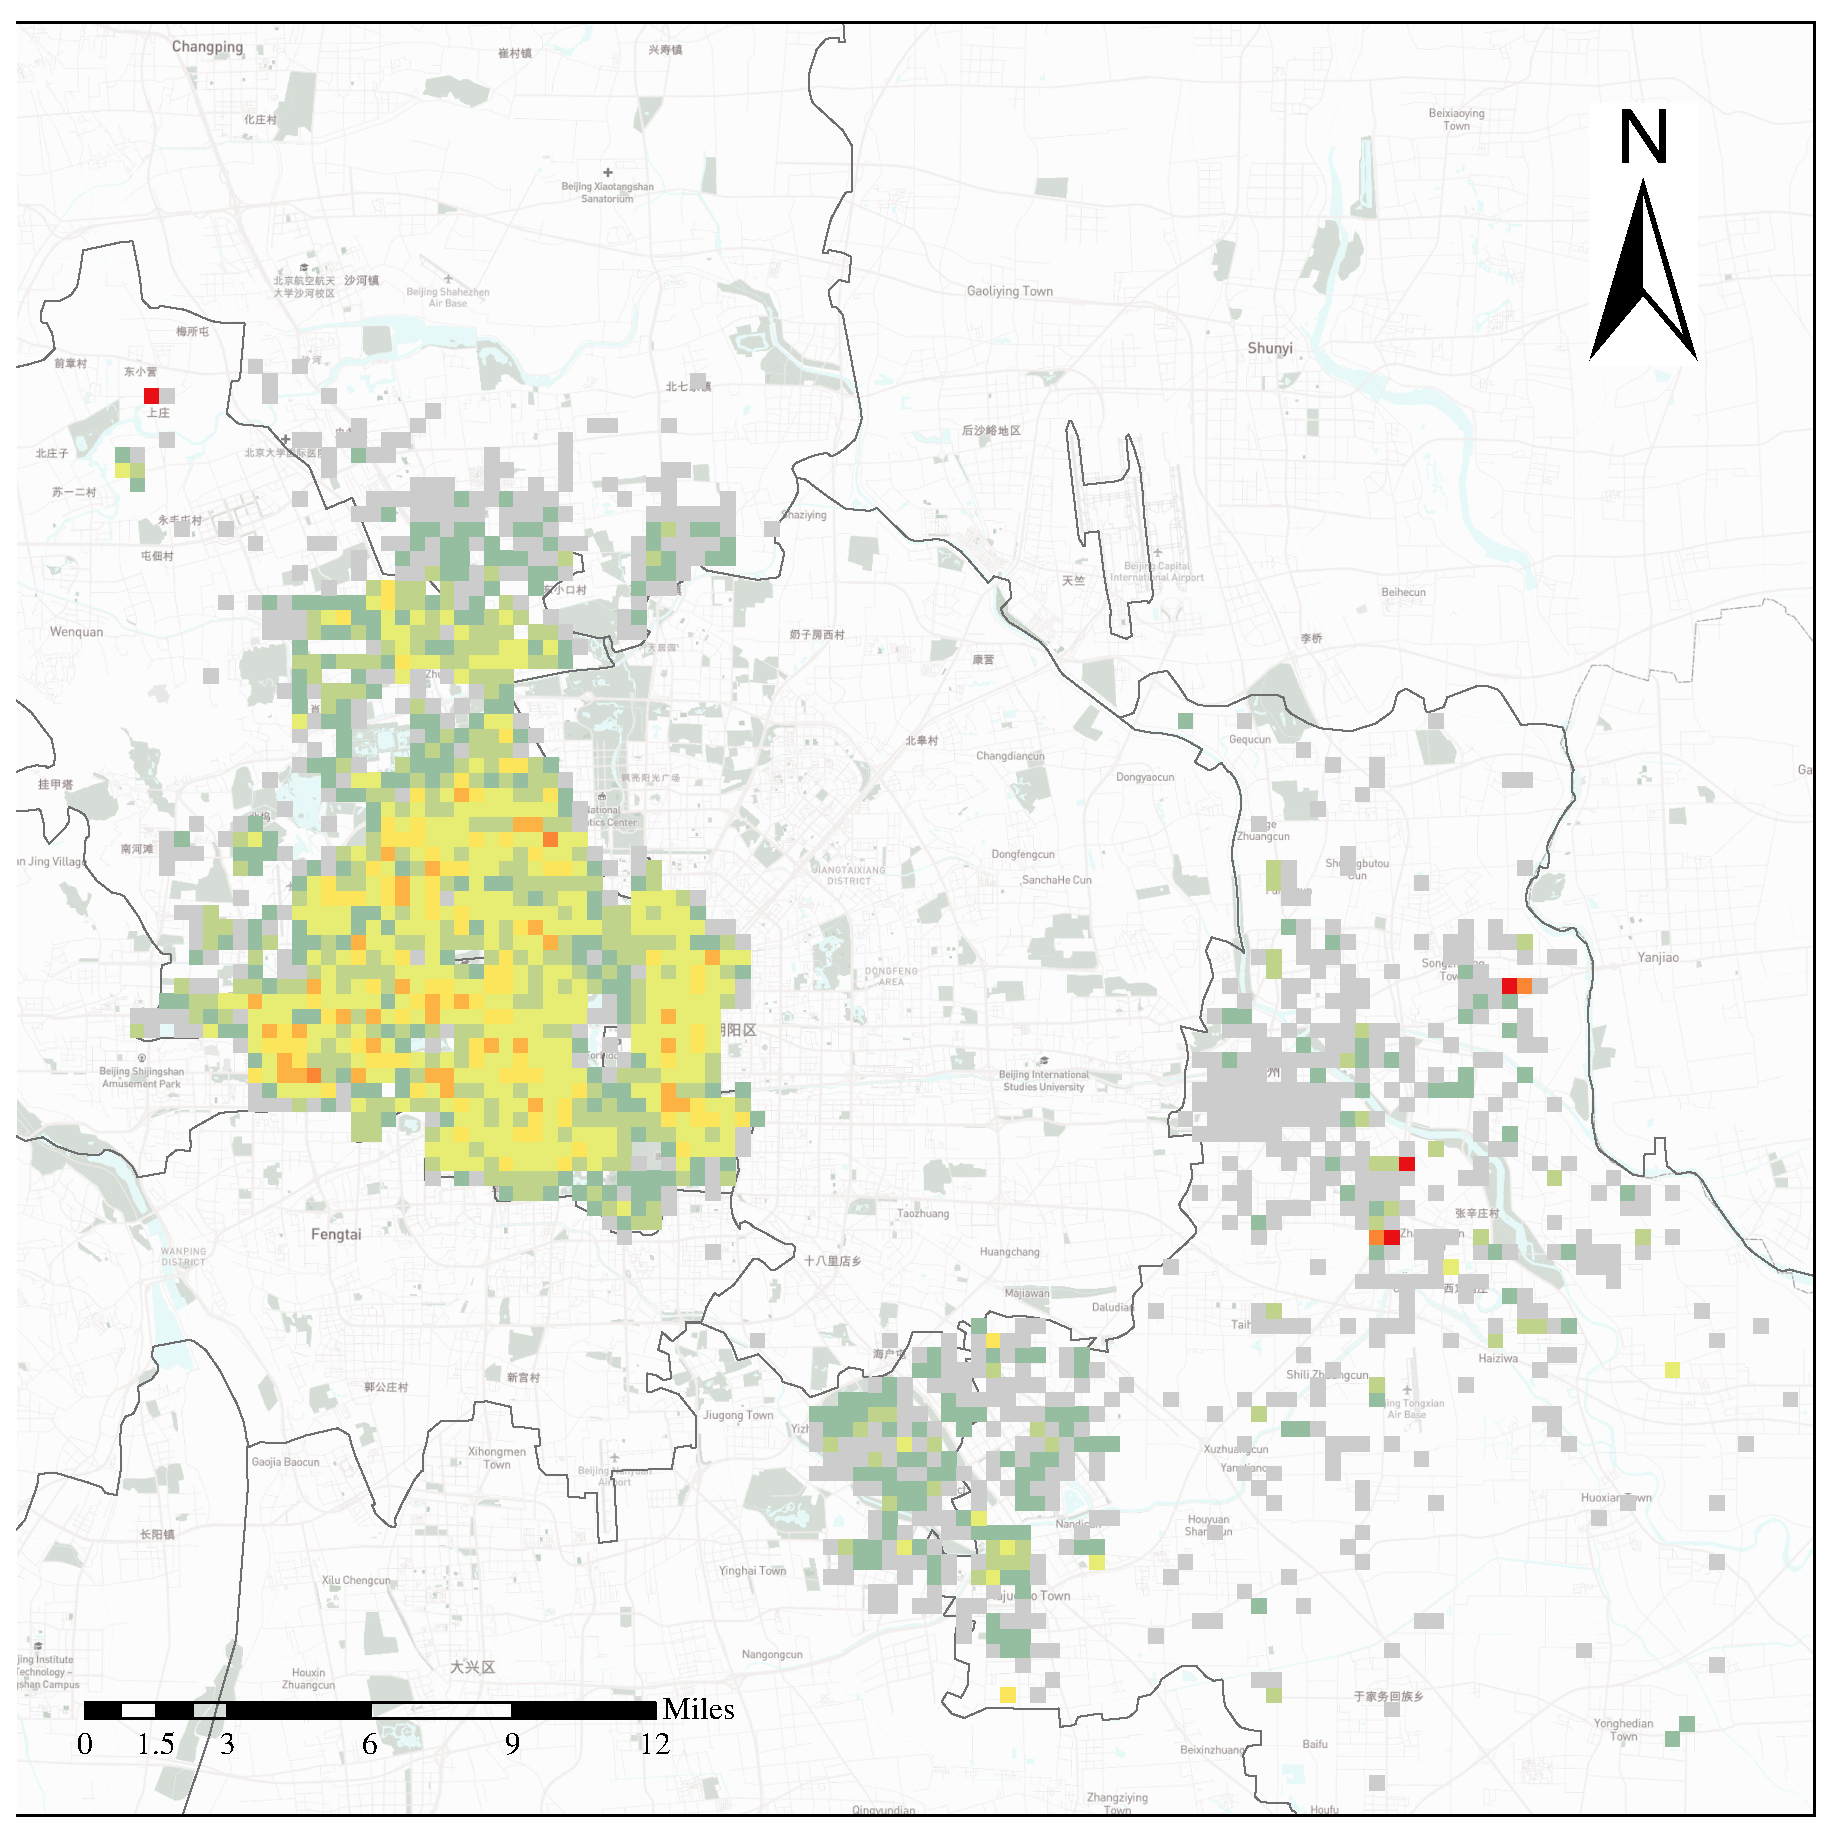
\includegraphics[width=\textwidth]{Figures/Overall_spatial_patterns/FN5_D2020_02_10.eps}
        \caption{10 Feb}
    \end{subfigure}
    \begin{subfigure}{.23\textwidth}
        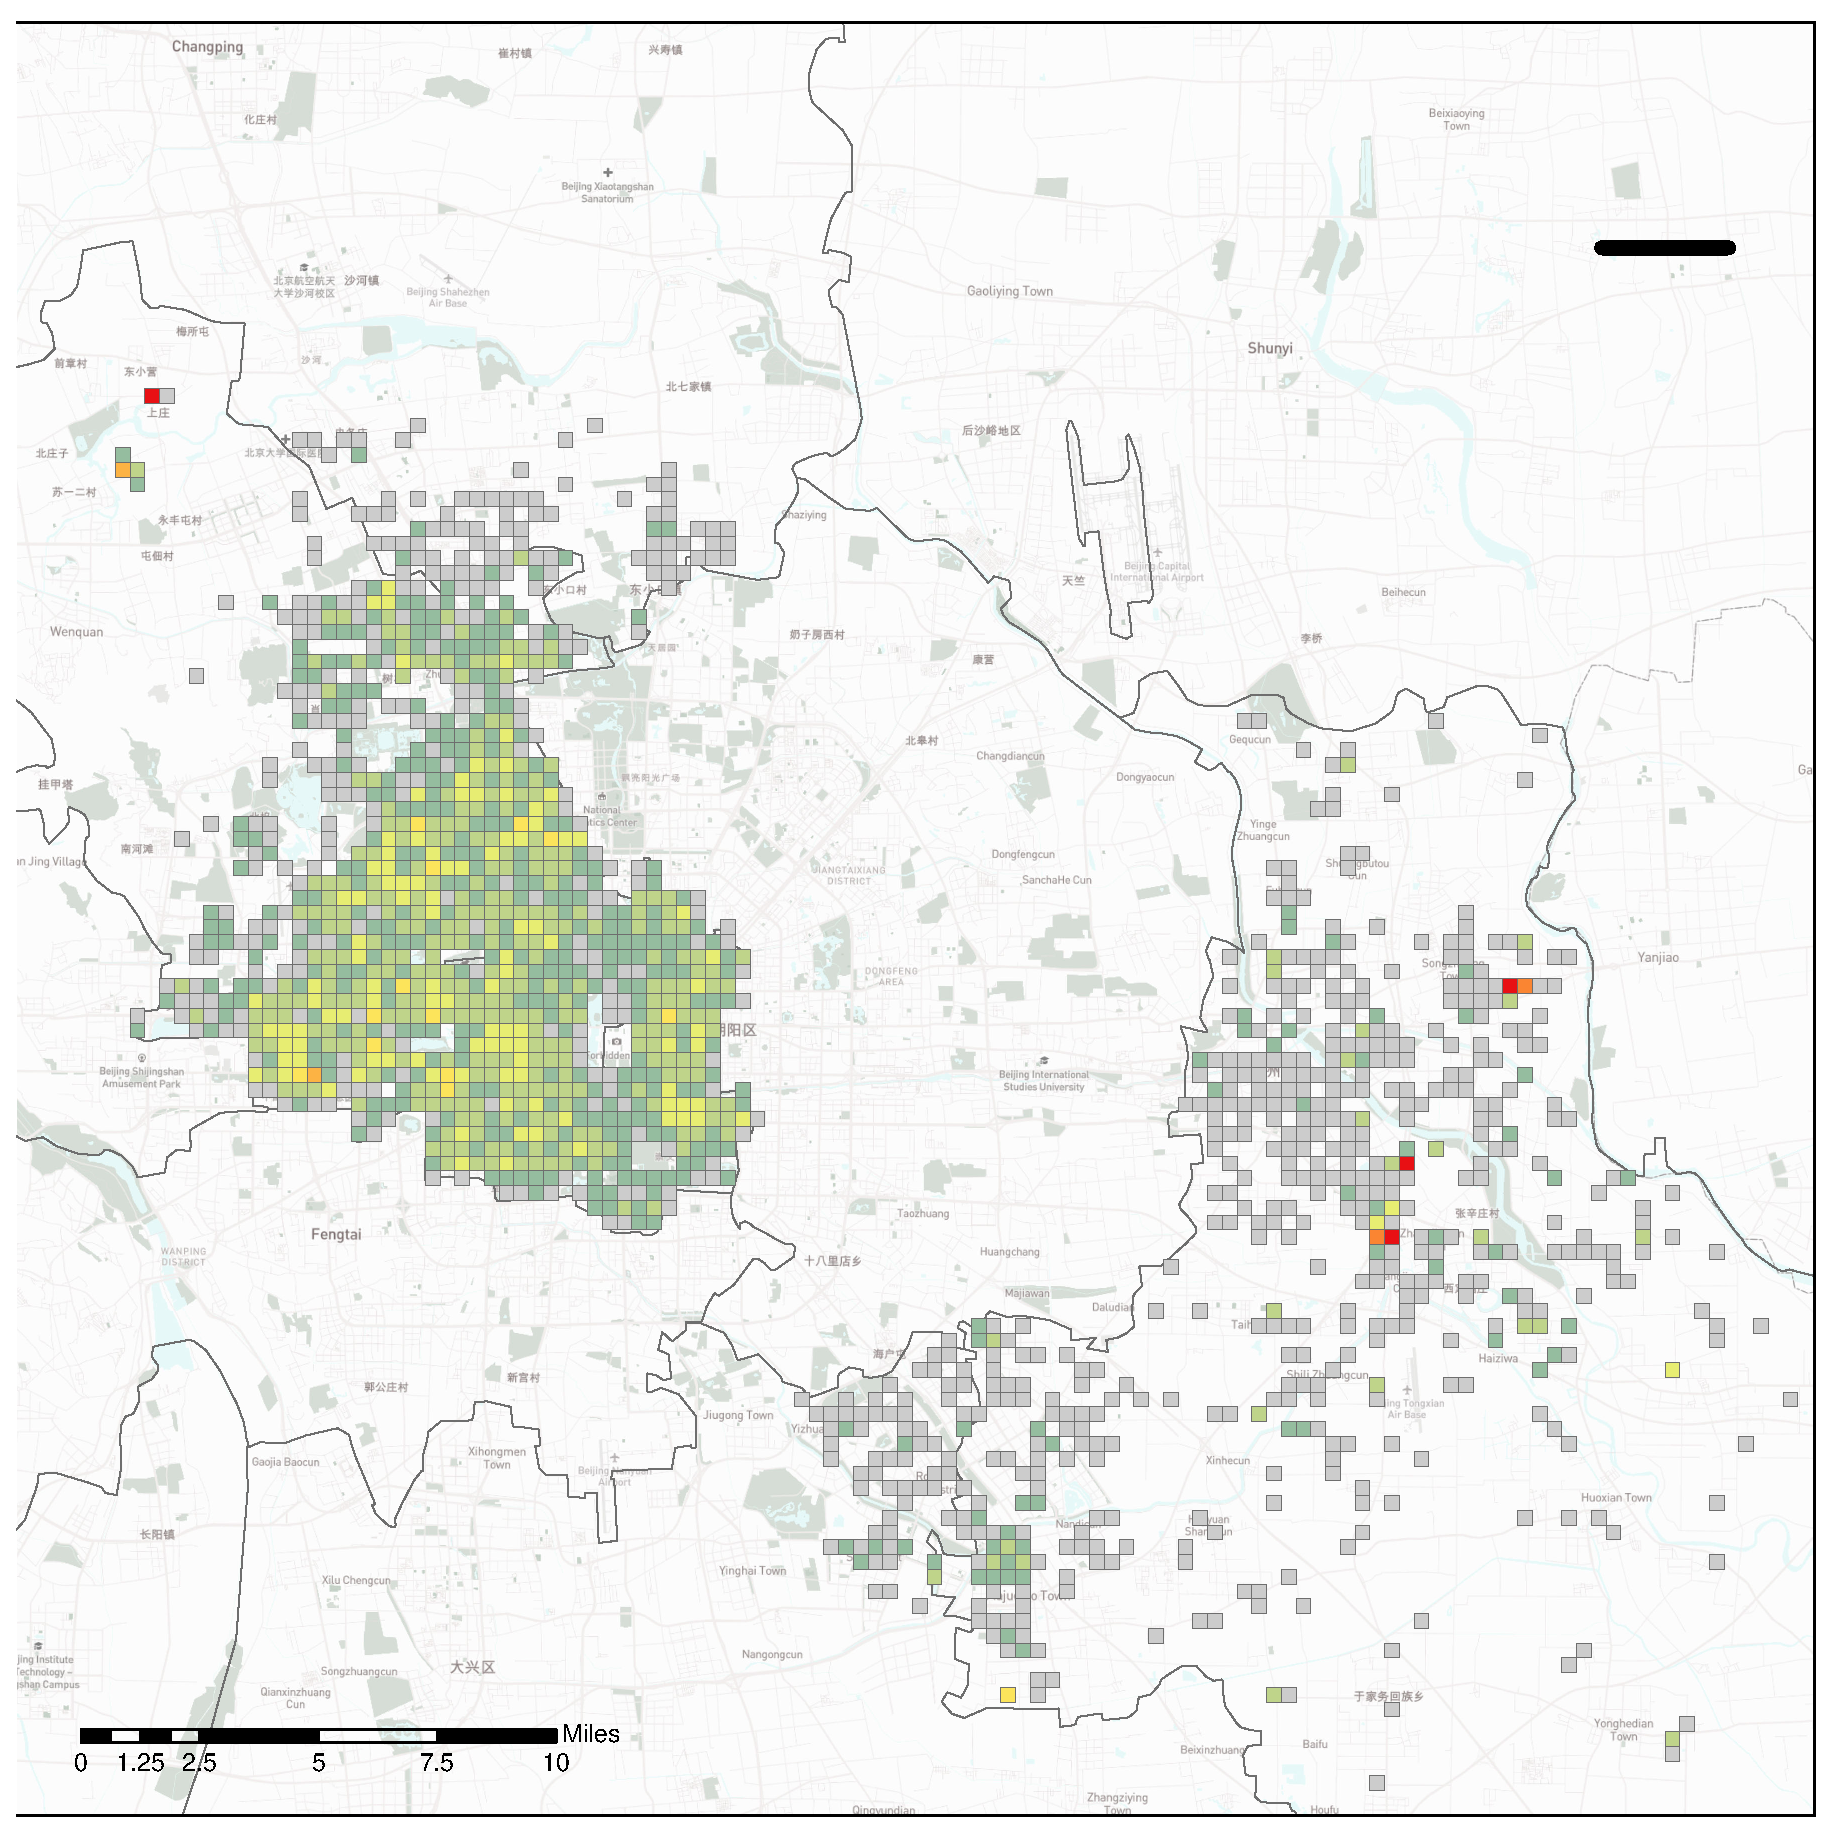
\includegraphics[width=\textwidth]{Figures/Overall_spatial_patterns/FN5_D2020_02_14.eps}
        \caption{14 Feb}
    \end{subfigure}
        \begin{subfigure}{.23\textwidth}
        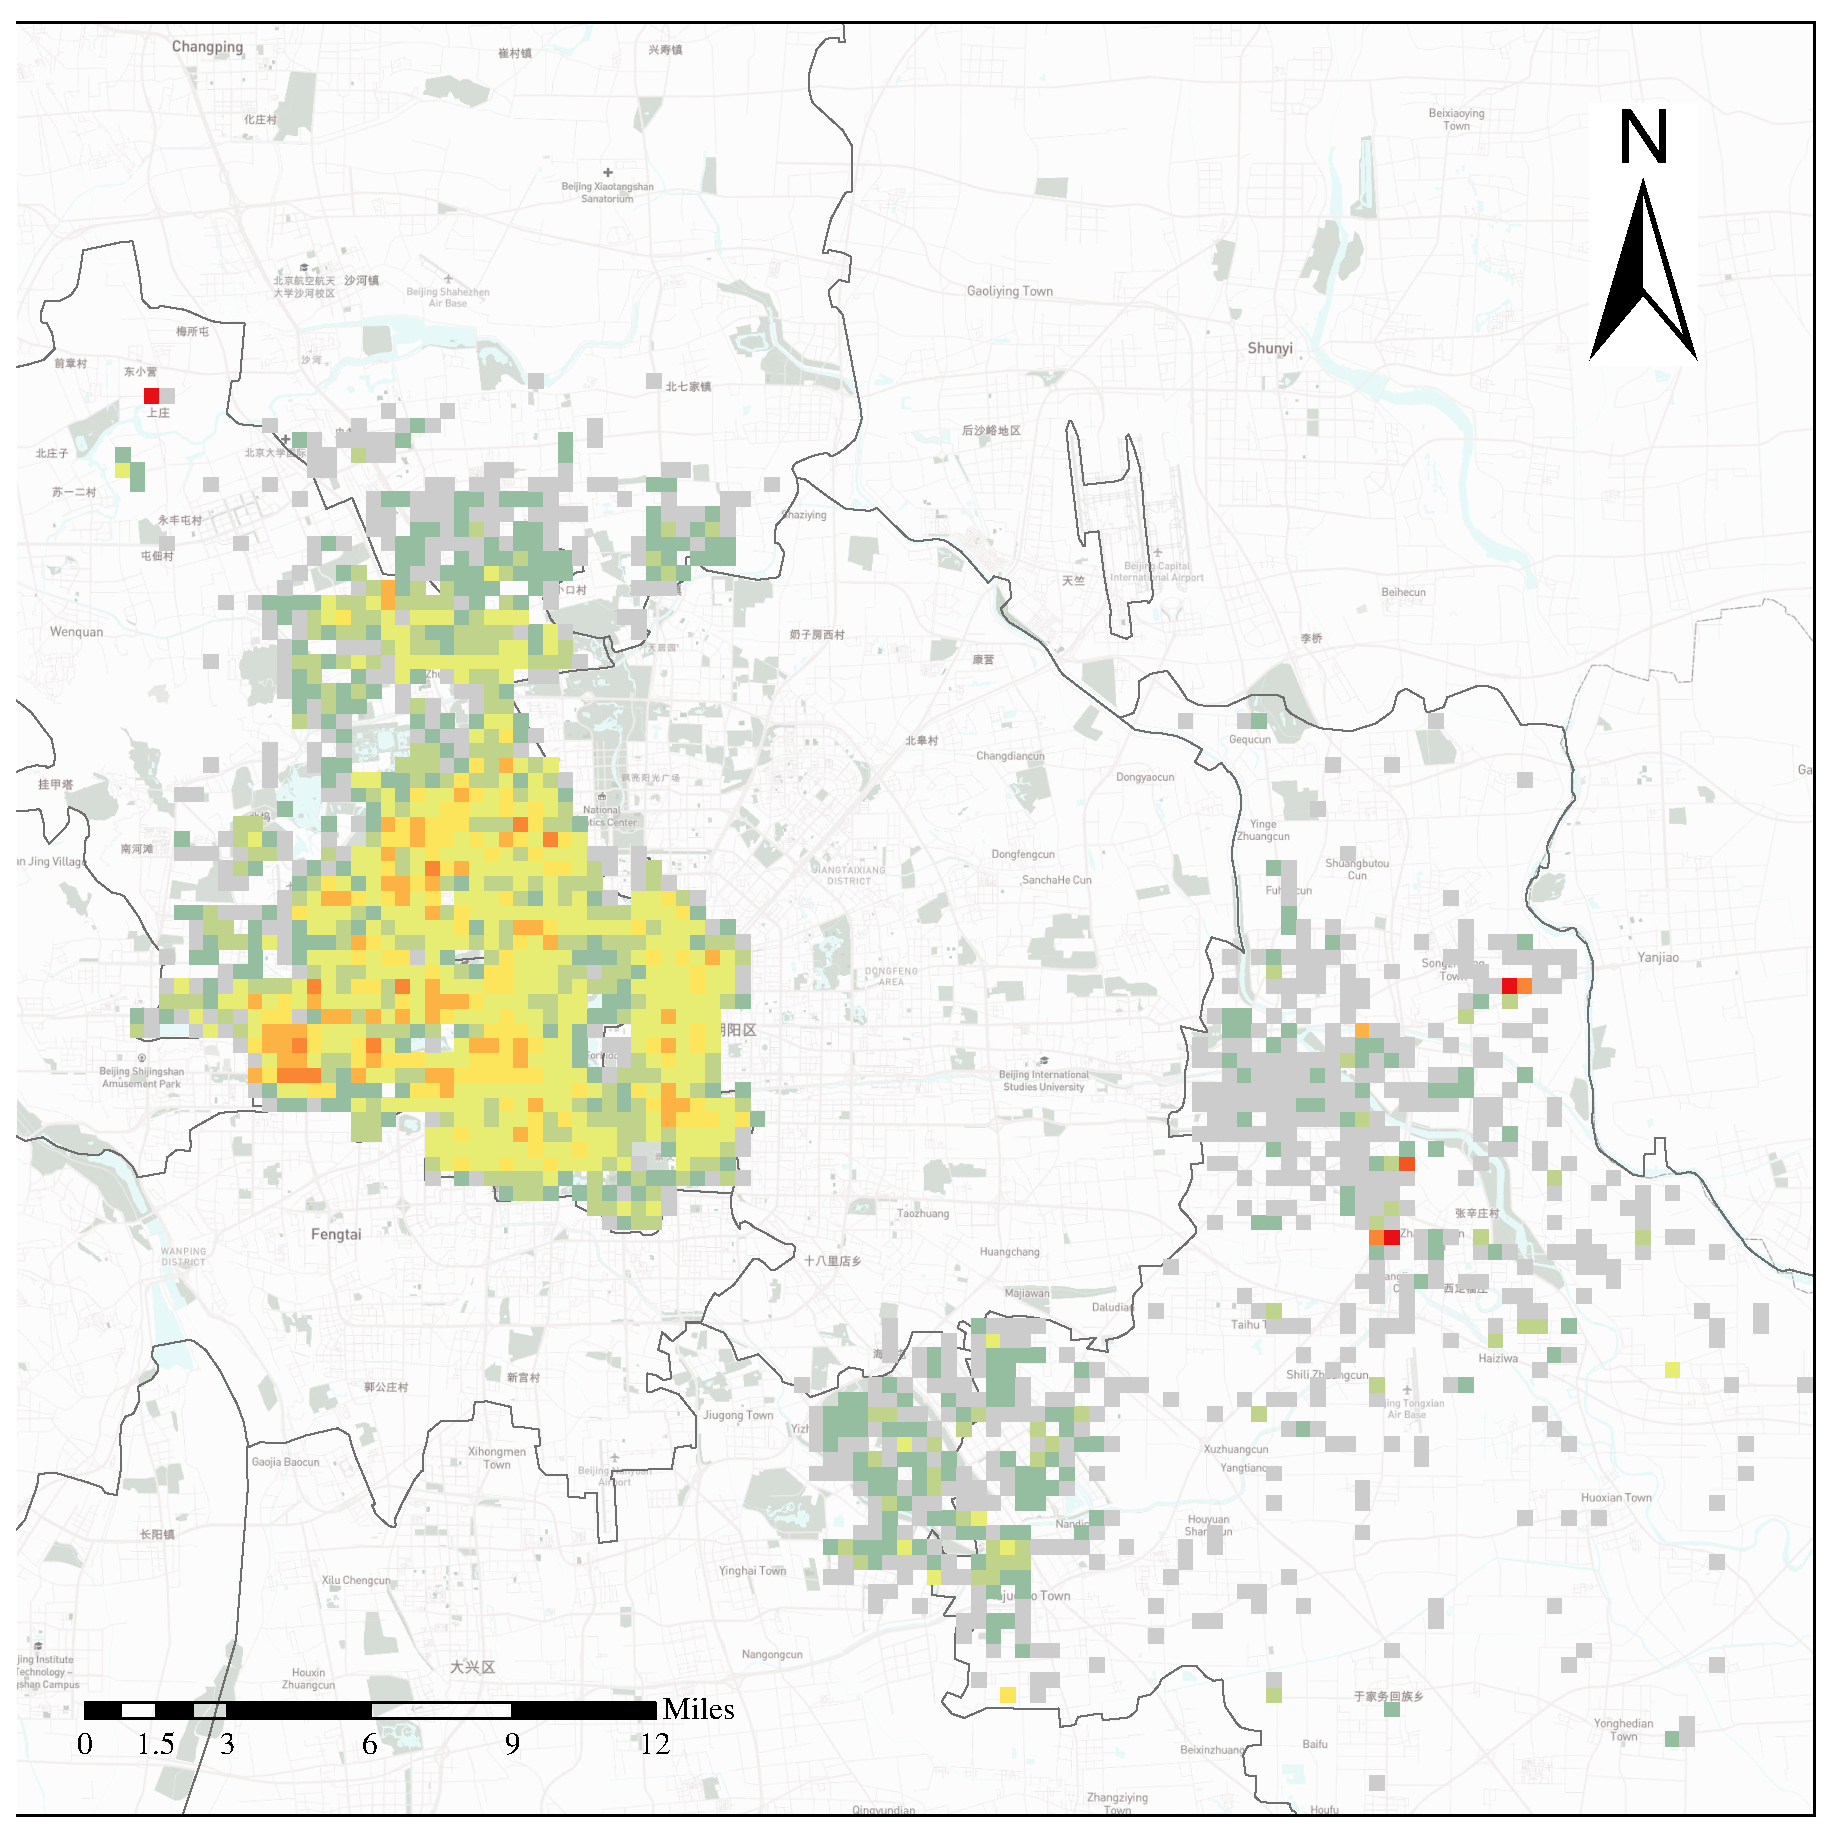
\includegraphics[width=\textwidth]{Figures/Overall_spatial_patterns/FN5_D2020_02_18.eps}
        \caption{18 Feb}
    \end{subfigure}
    
    \vspace{6pt}
    \begin{subfigure}{.23\textwidth}
        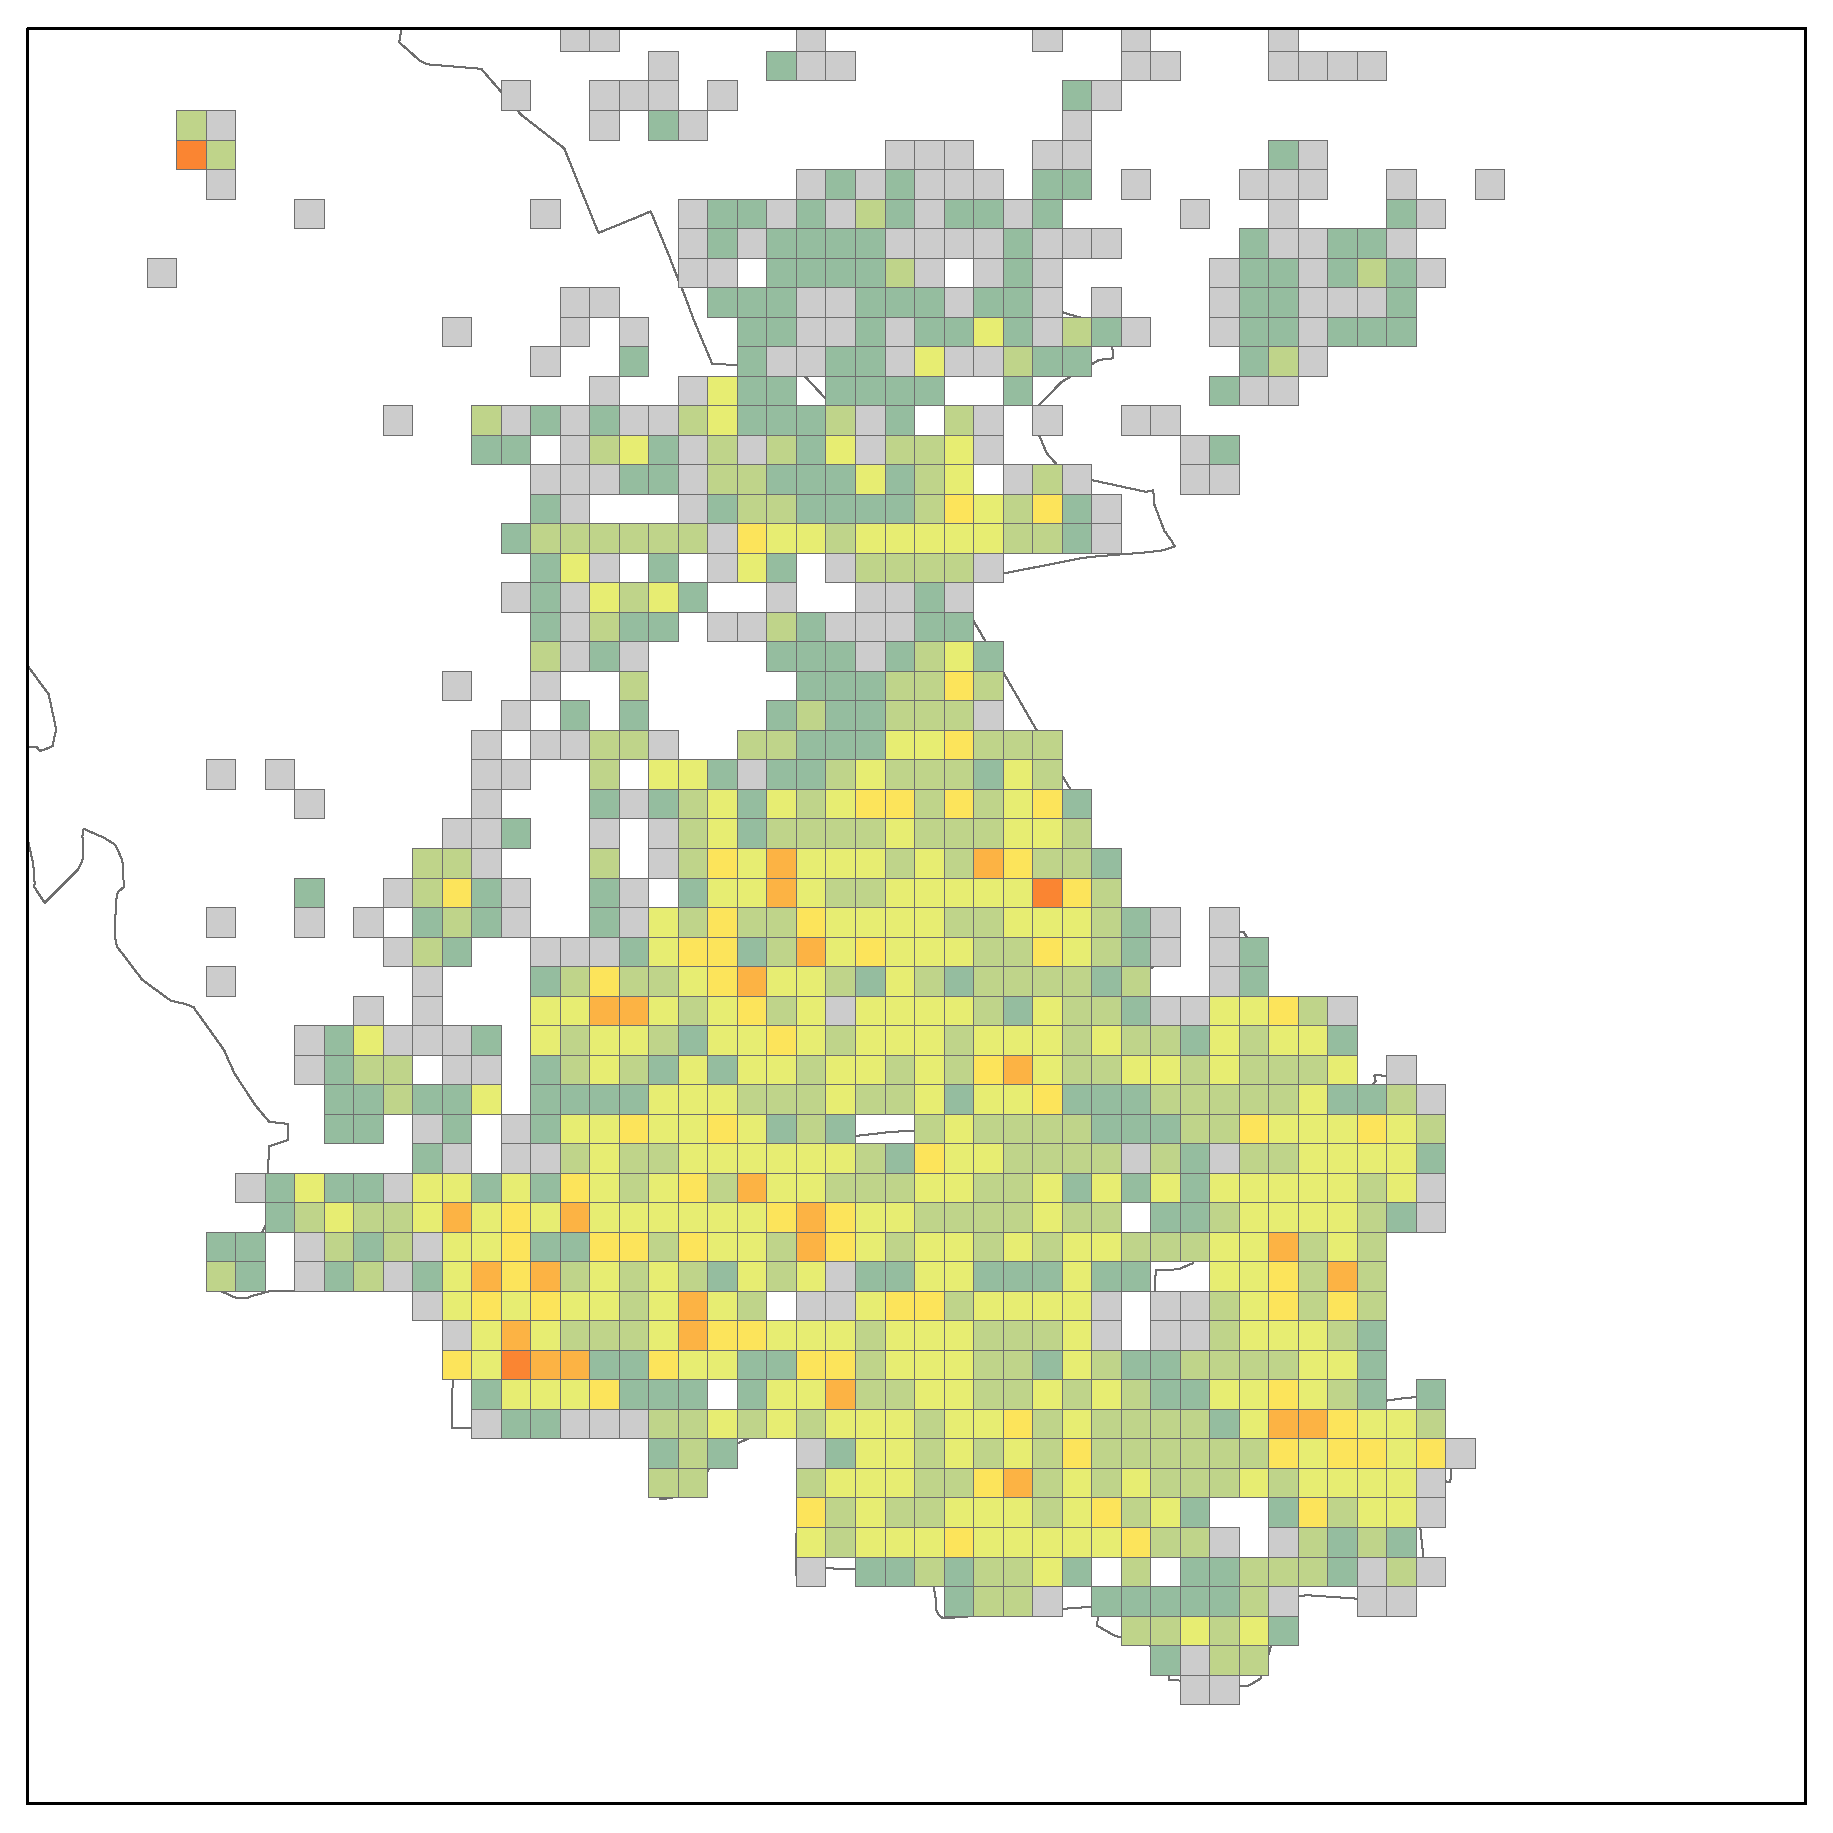
\includegraphics[width=\textwidth]{Figures/Overall_spatial_patterns/FN5_D2020_02_22.eps}
        \caption{24 Feb}
    \end{subfigure}
    \begin{subfigure}{.23\textwidth}
        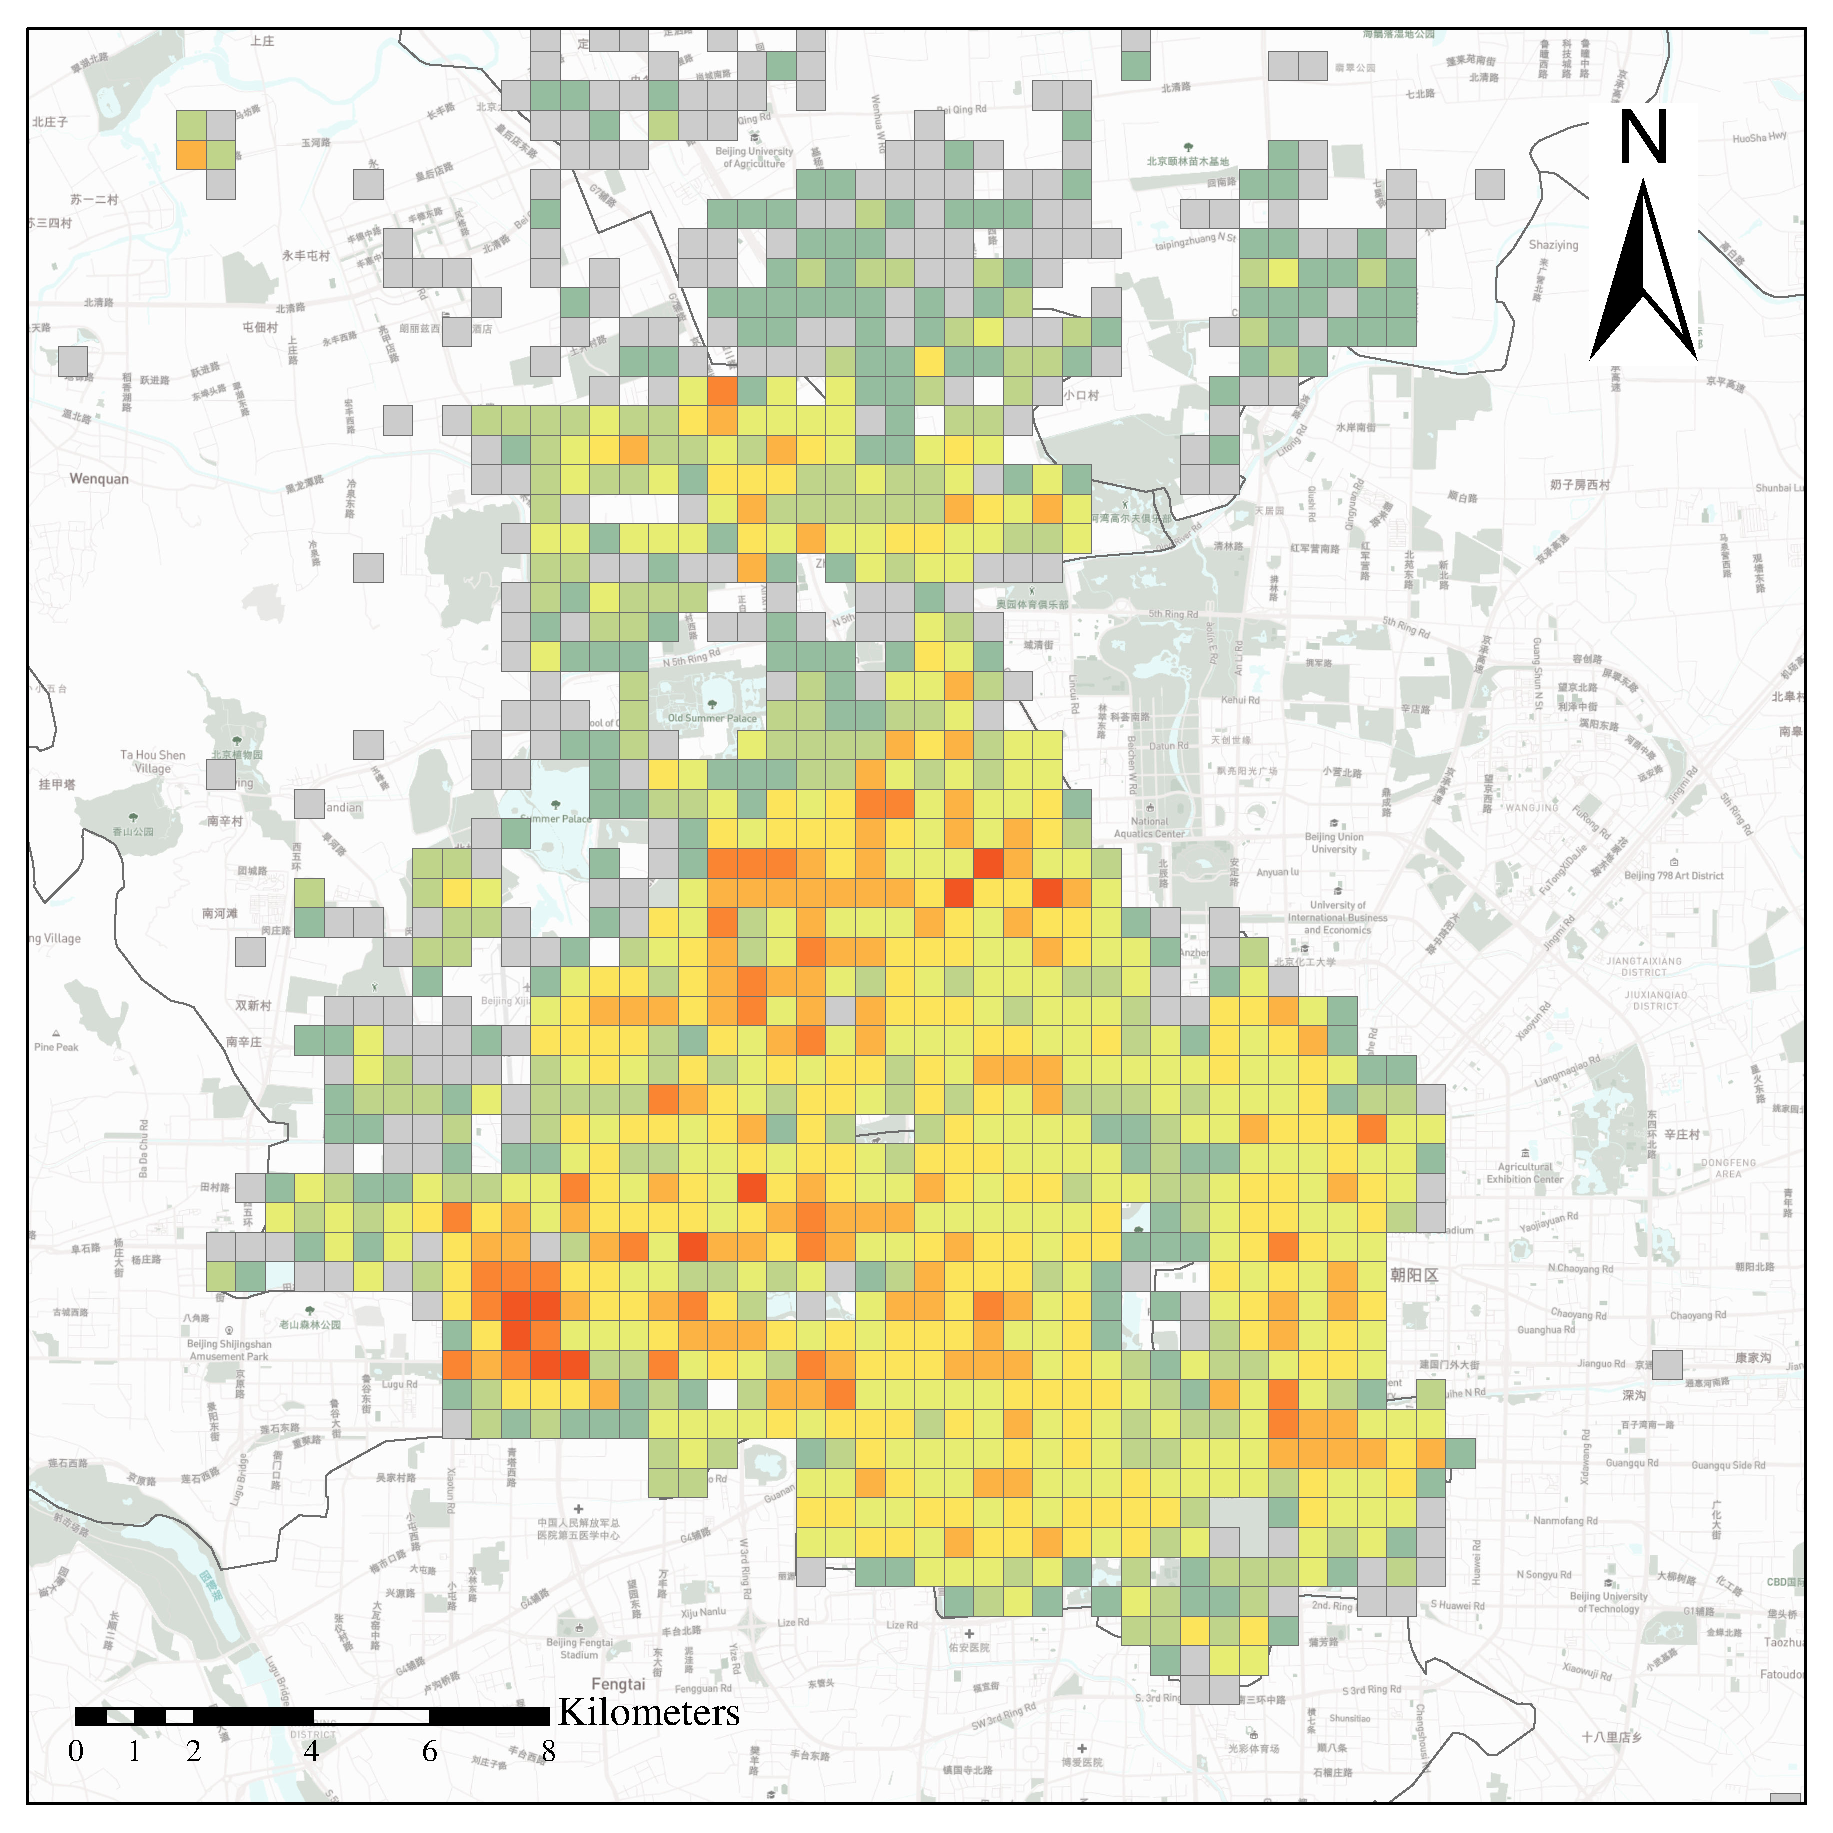
\includegraphics[width=\textwidth]{Figures/Overall_spatial_patterns/FN5_D2020_02_26.eps}
        \caption{26 Feb}
    \end{subfigure}
    \begin{subfigure}{.23\textwidth}
        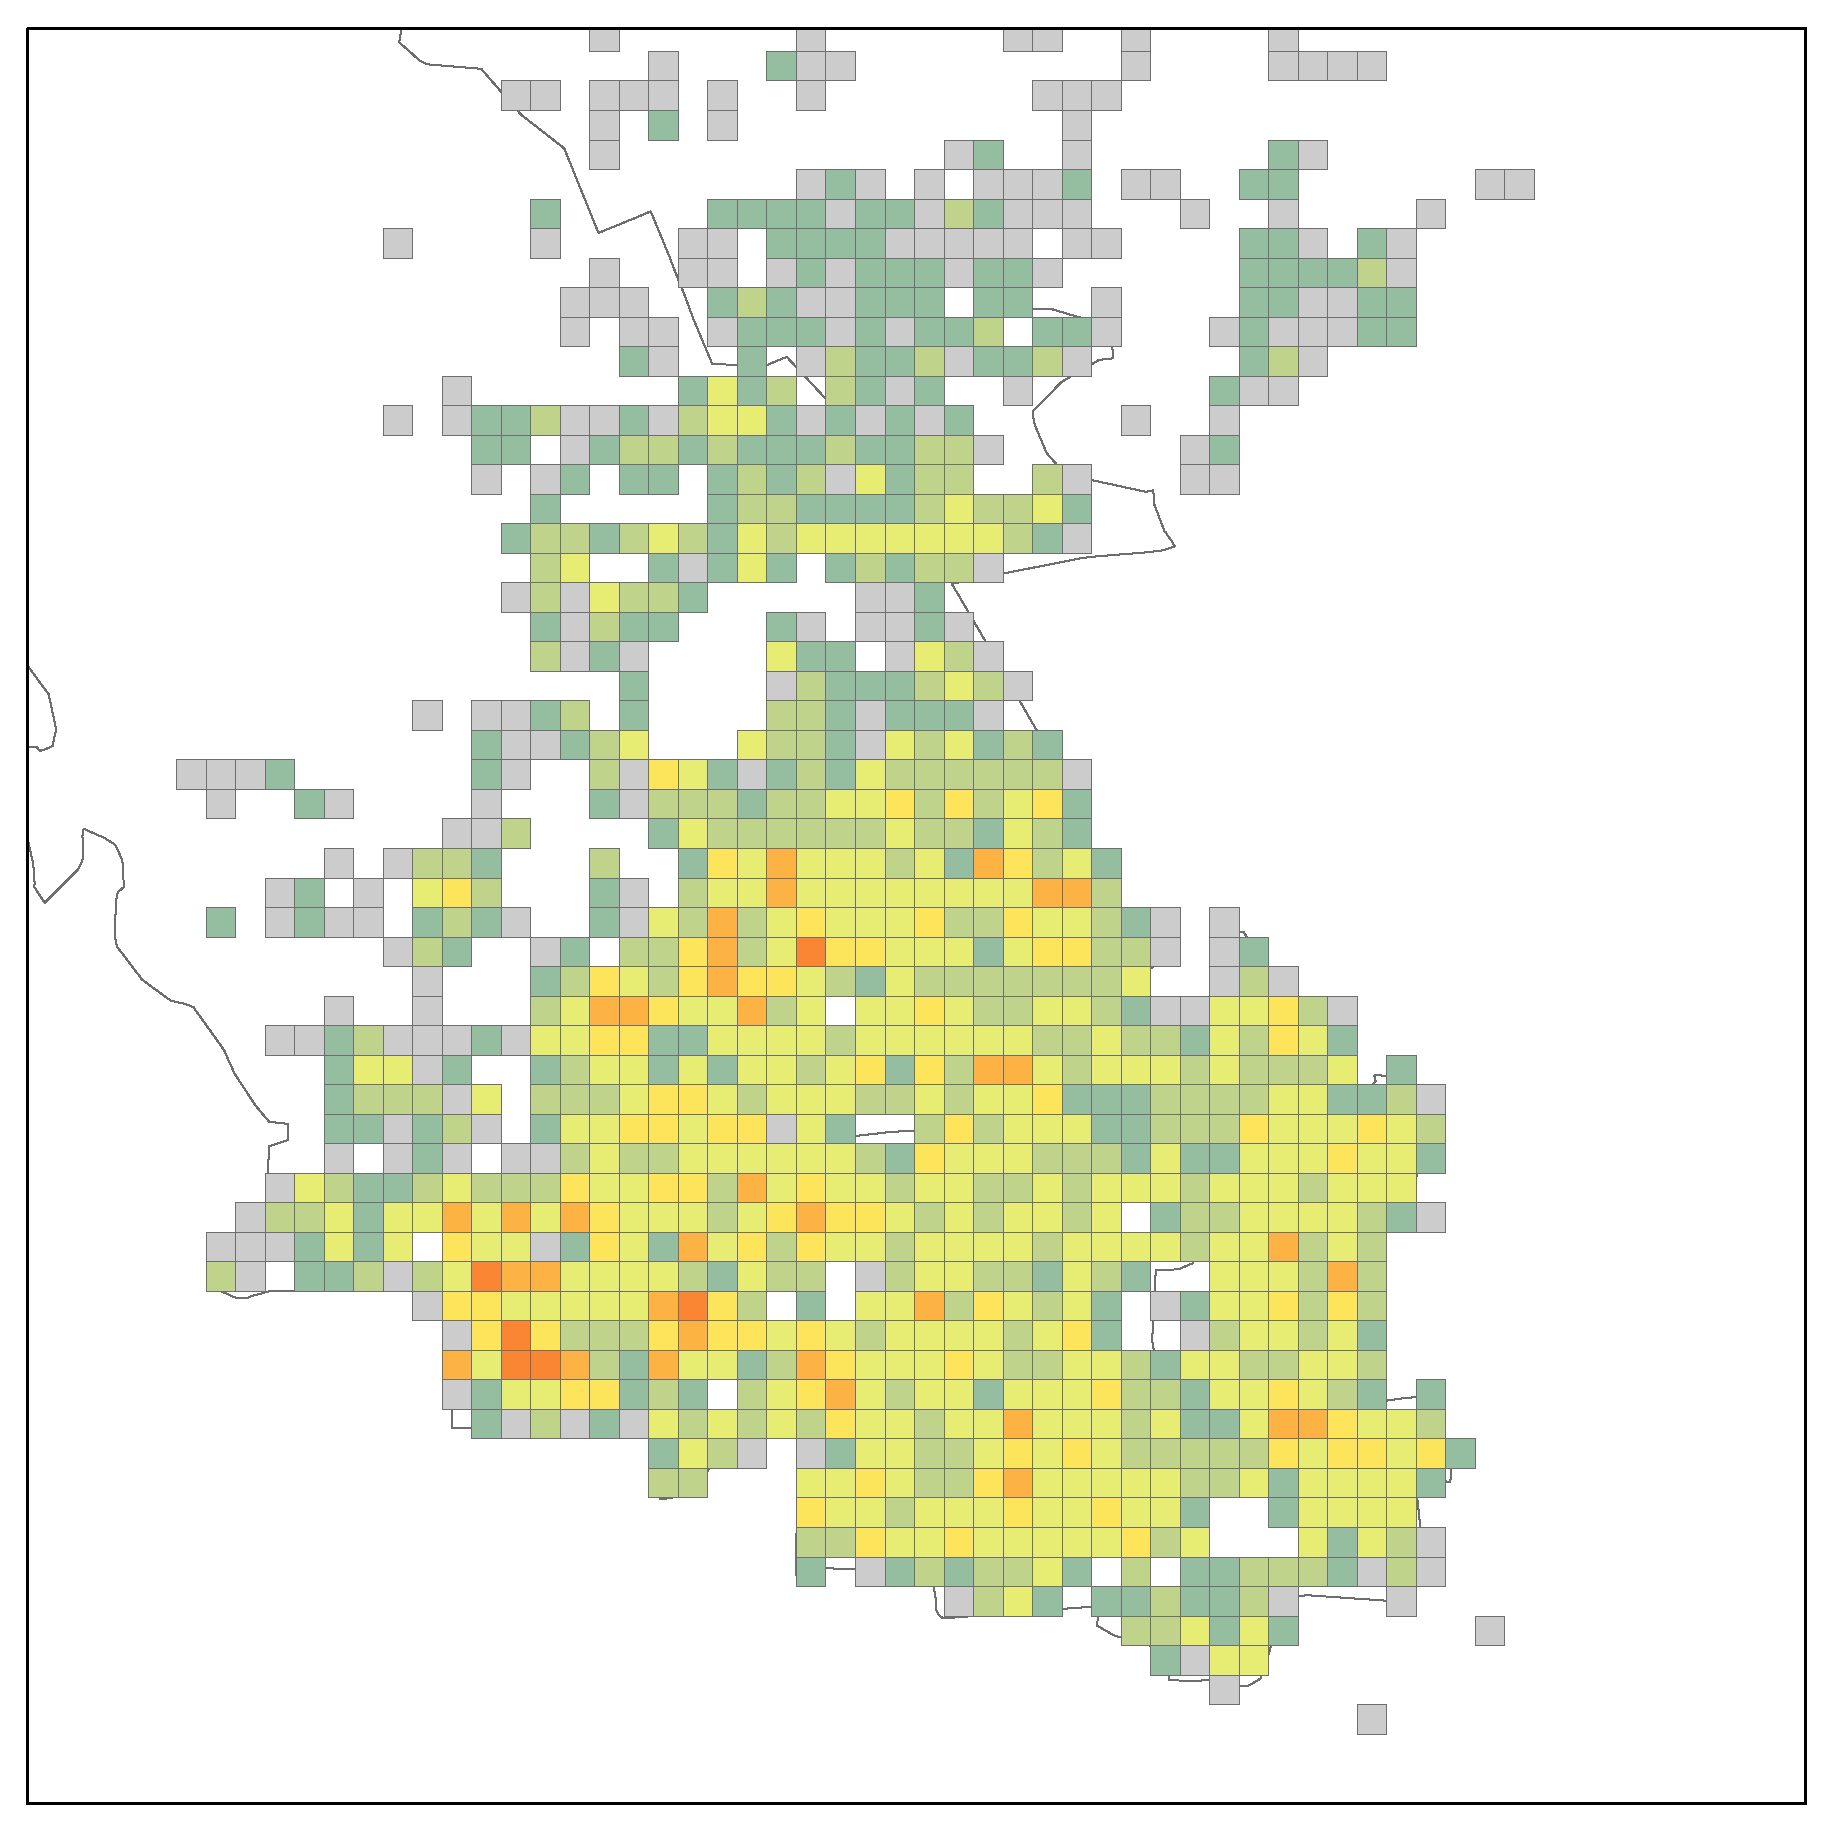
\includegraphics[width=\textwidth]{Figures/Overall_spatial_patterns/FN5_D2020_03_01.eps}
        \caption{01 Mar}
    \end{subfigure}
    \begin{subfigure}{.2\textwidth}
        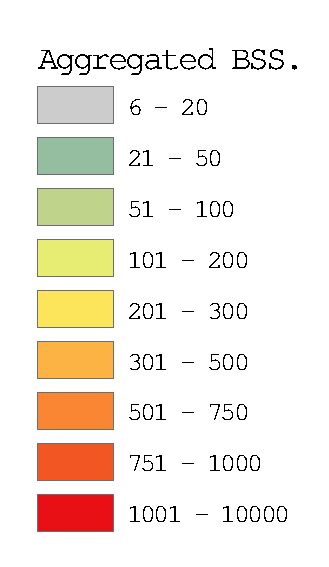
\includegraphics[width=\textwidth]{Figures/Overall_spatial_patterns/legend5.eps}
        \caption{Legend}
    \end{subfigure}
    
    \caption{Spatial patterns of cycling activities from 21 Jan to 01 March 2020}
    \label{fig:full_spatial_pattern_2020}
\end{figure}

\subsection{Discussions}
Part 1. Comparison with data from the same period in 2019.
\textcolor{red}{In order to remove the influence of Lunar New Year holiday, comparison is conducted with data from the same period in 2019. Before...Holiday...Return-to-work...}
\begin{figure}[H]
    \centering
    \begin{subfigure}{.3\textwidth}
        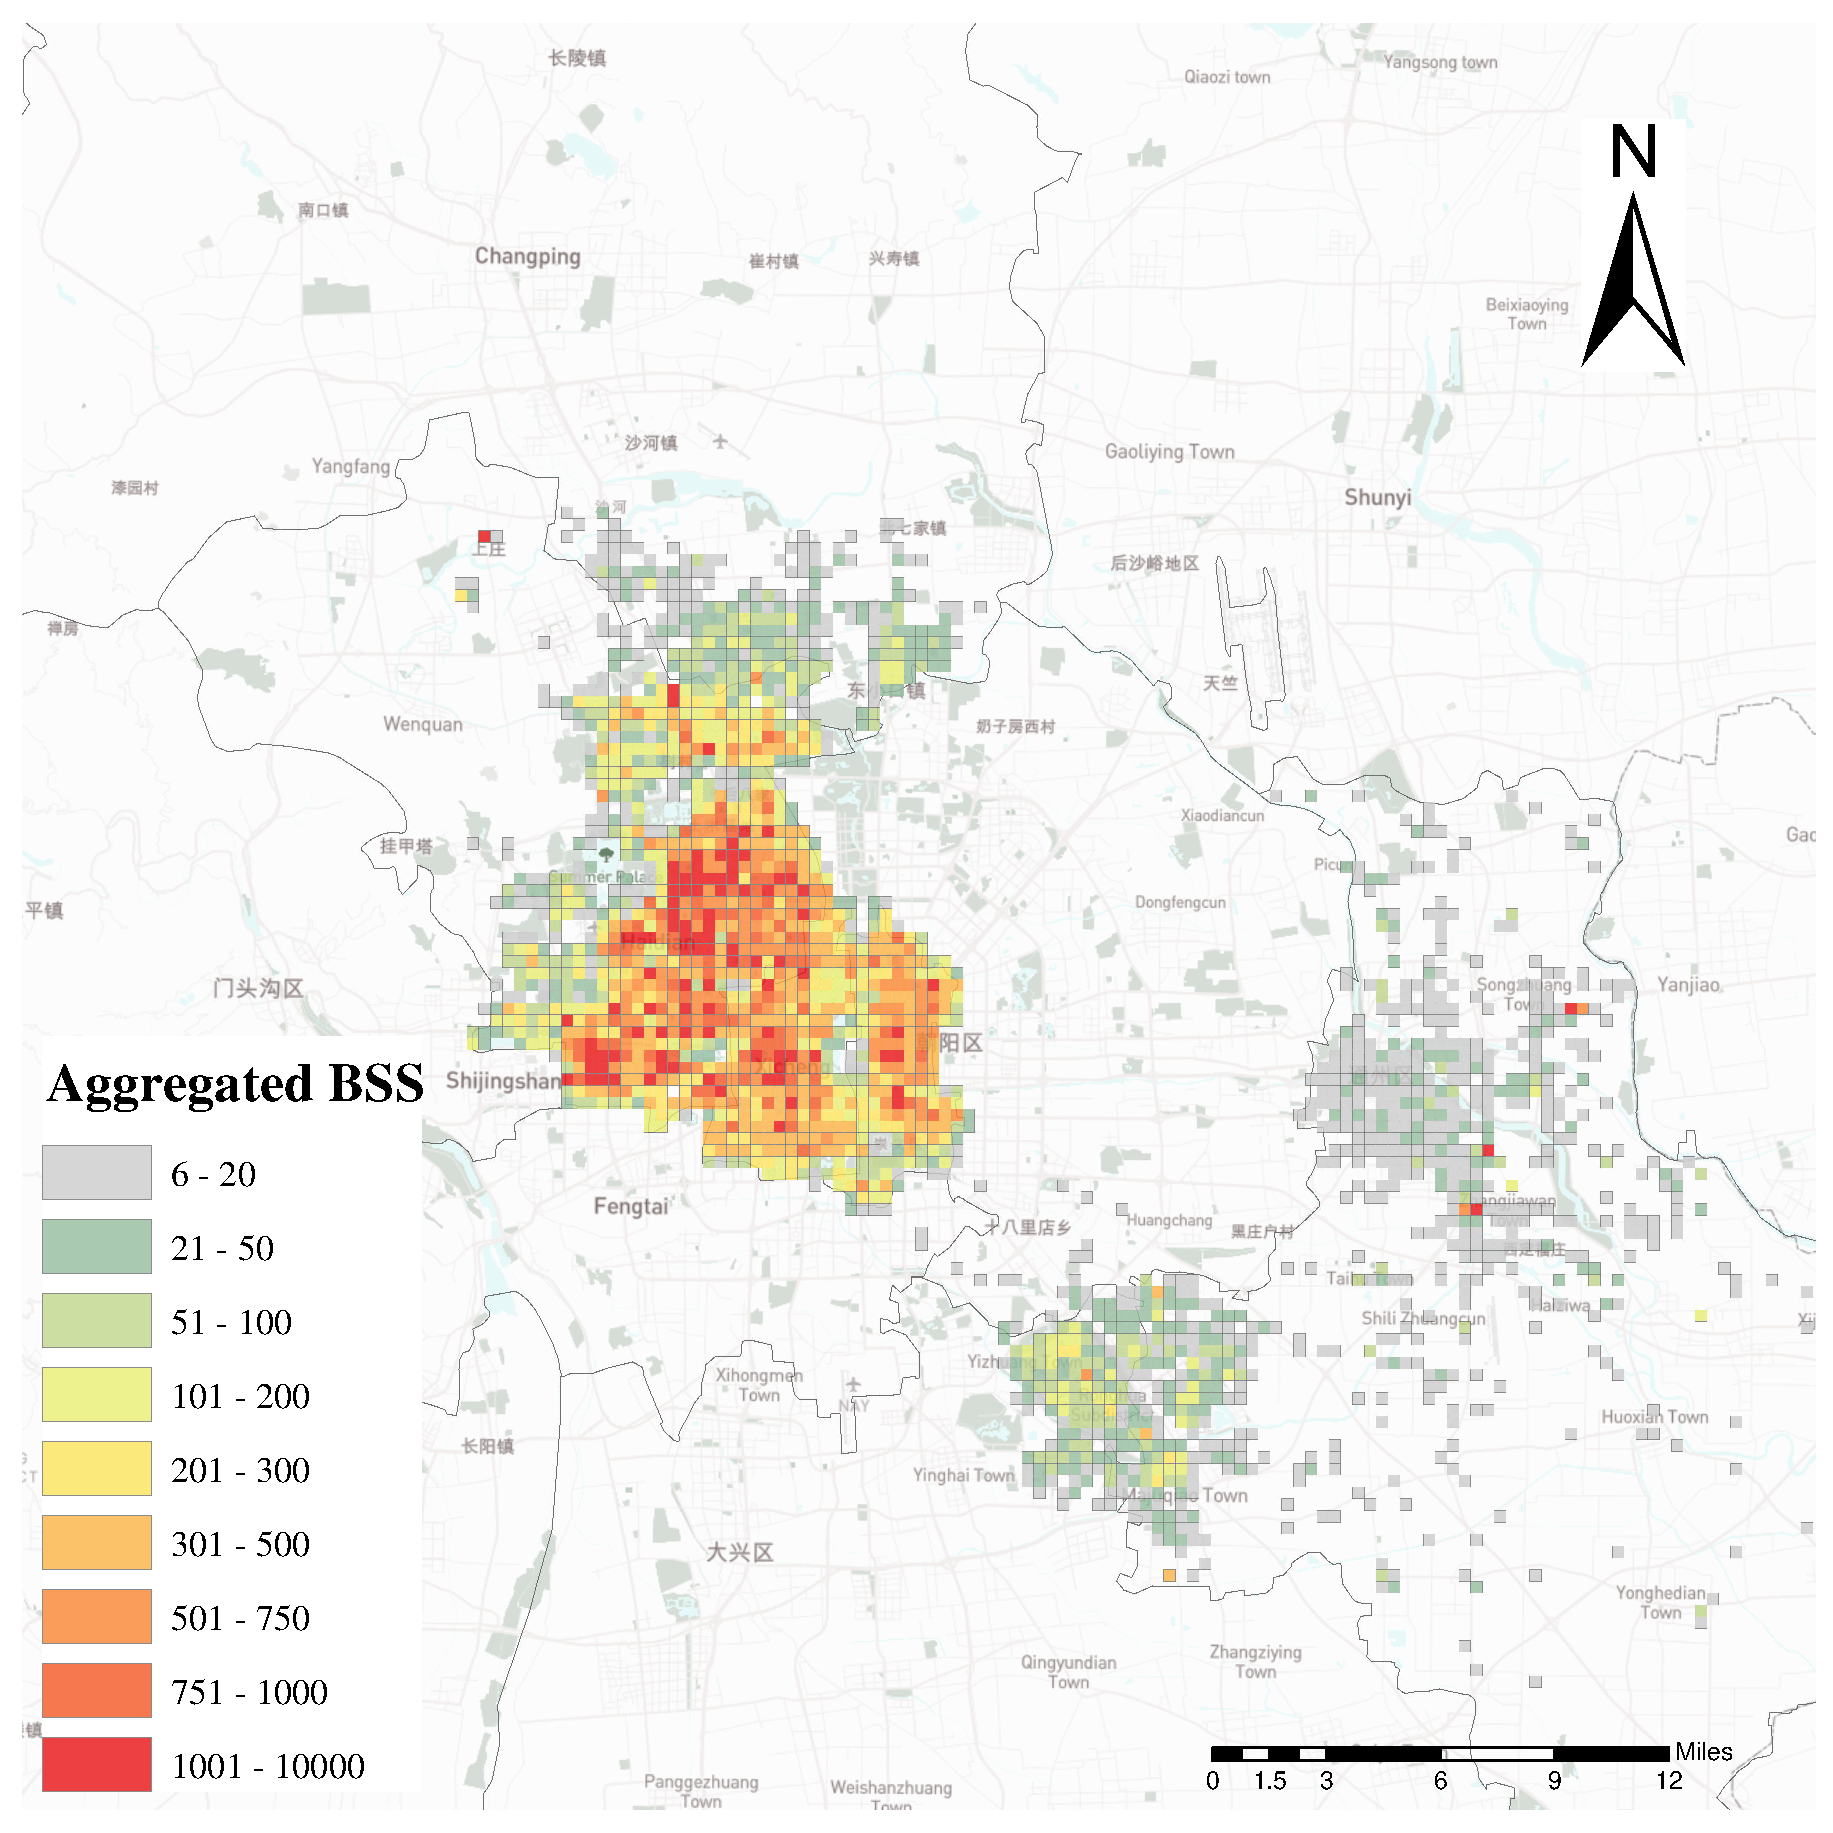
\includegraphics[width=\textwidth]{Figures/BSSPhase1_2020.eps}
        \caption{Before spring festival 2020}
    \end{subfigure}
    \begin{subfigure}{.3\textwidth}
        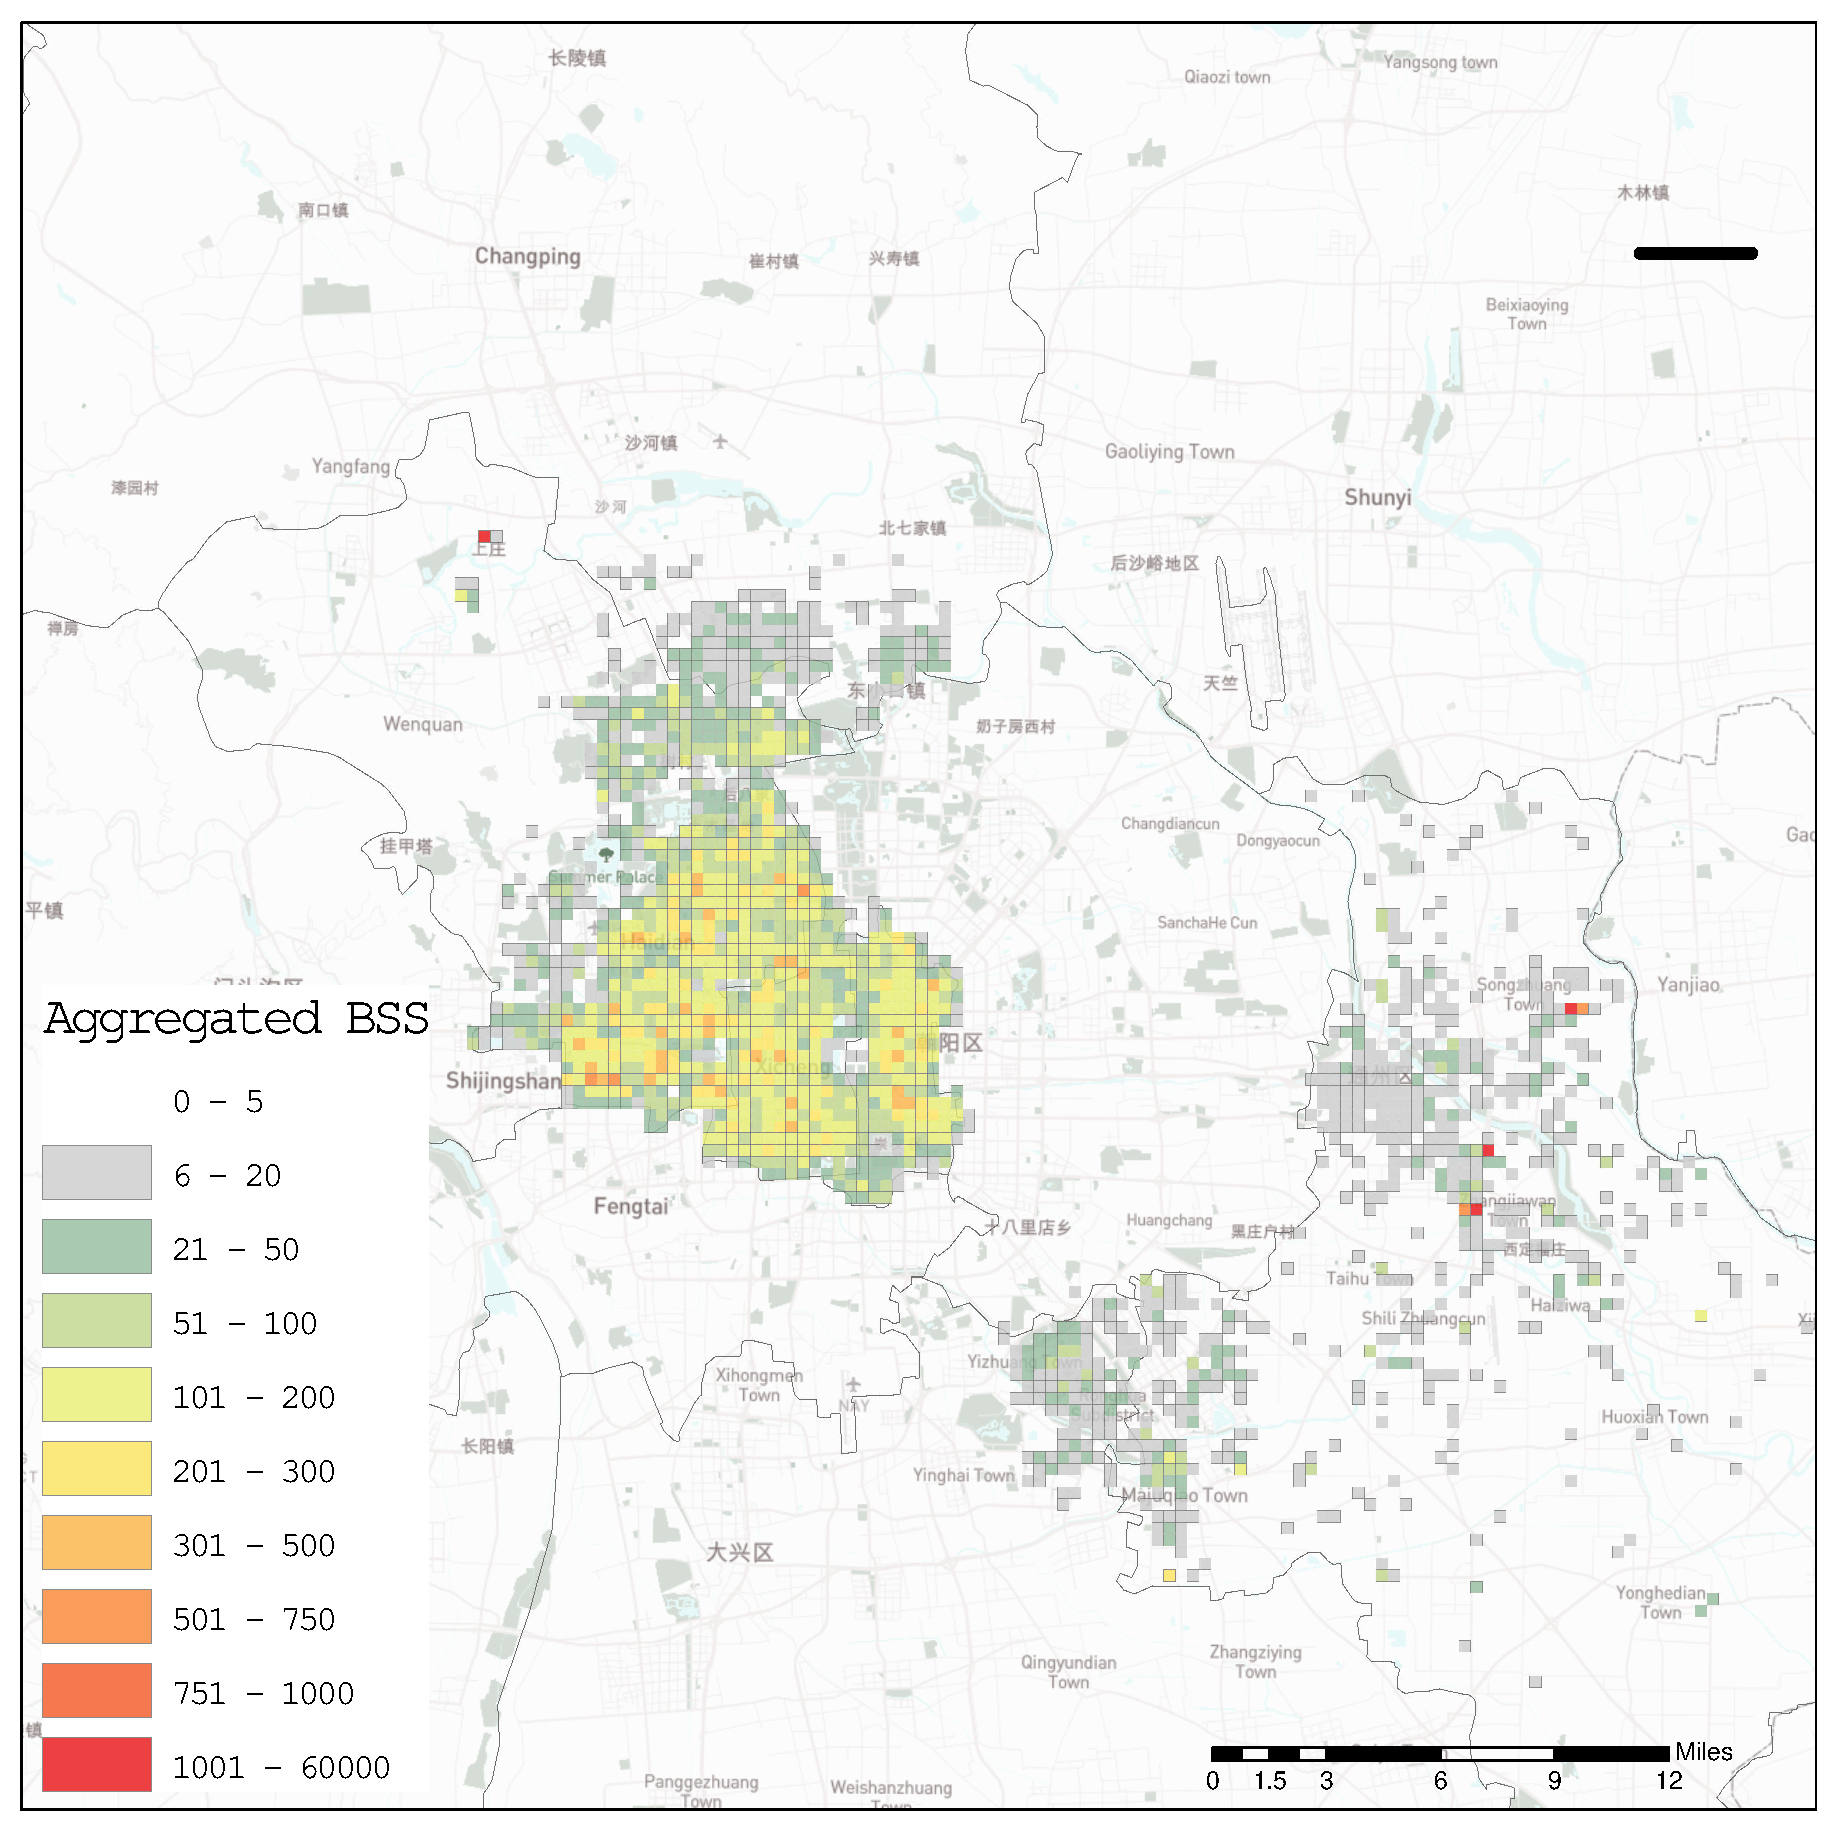
\includegraphics[width=\textwidth]{Figures/BSSPhase2_2020.eps}
        \caption{Spring festival 2020}
    \end{subfigure}
    \begin{subfigure}{.3\textwidth}
        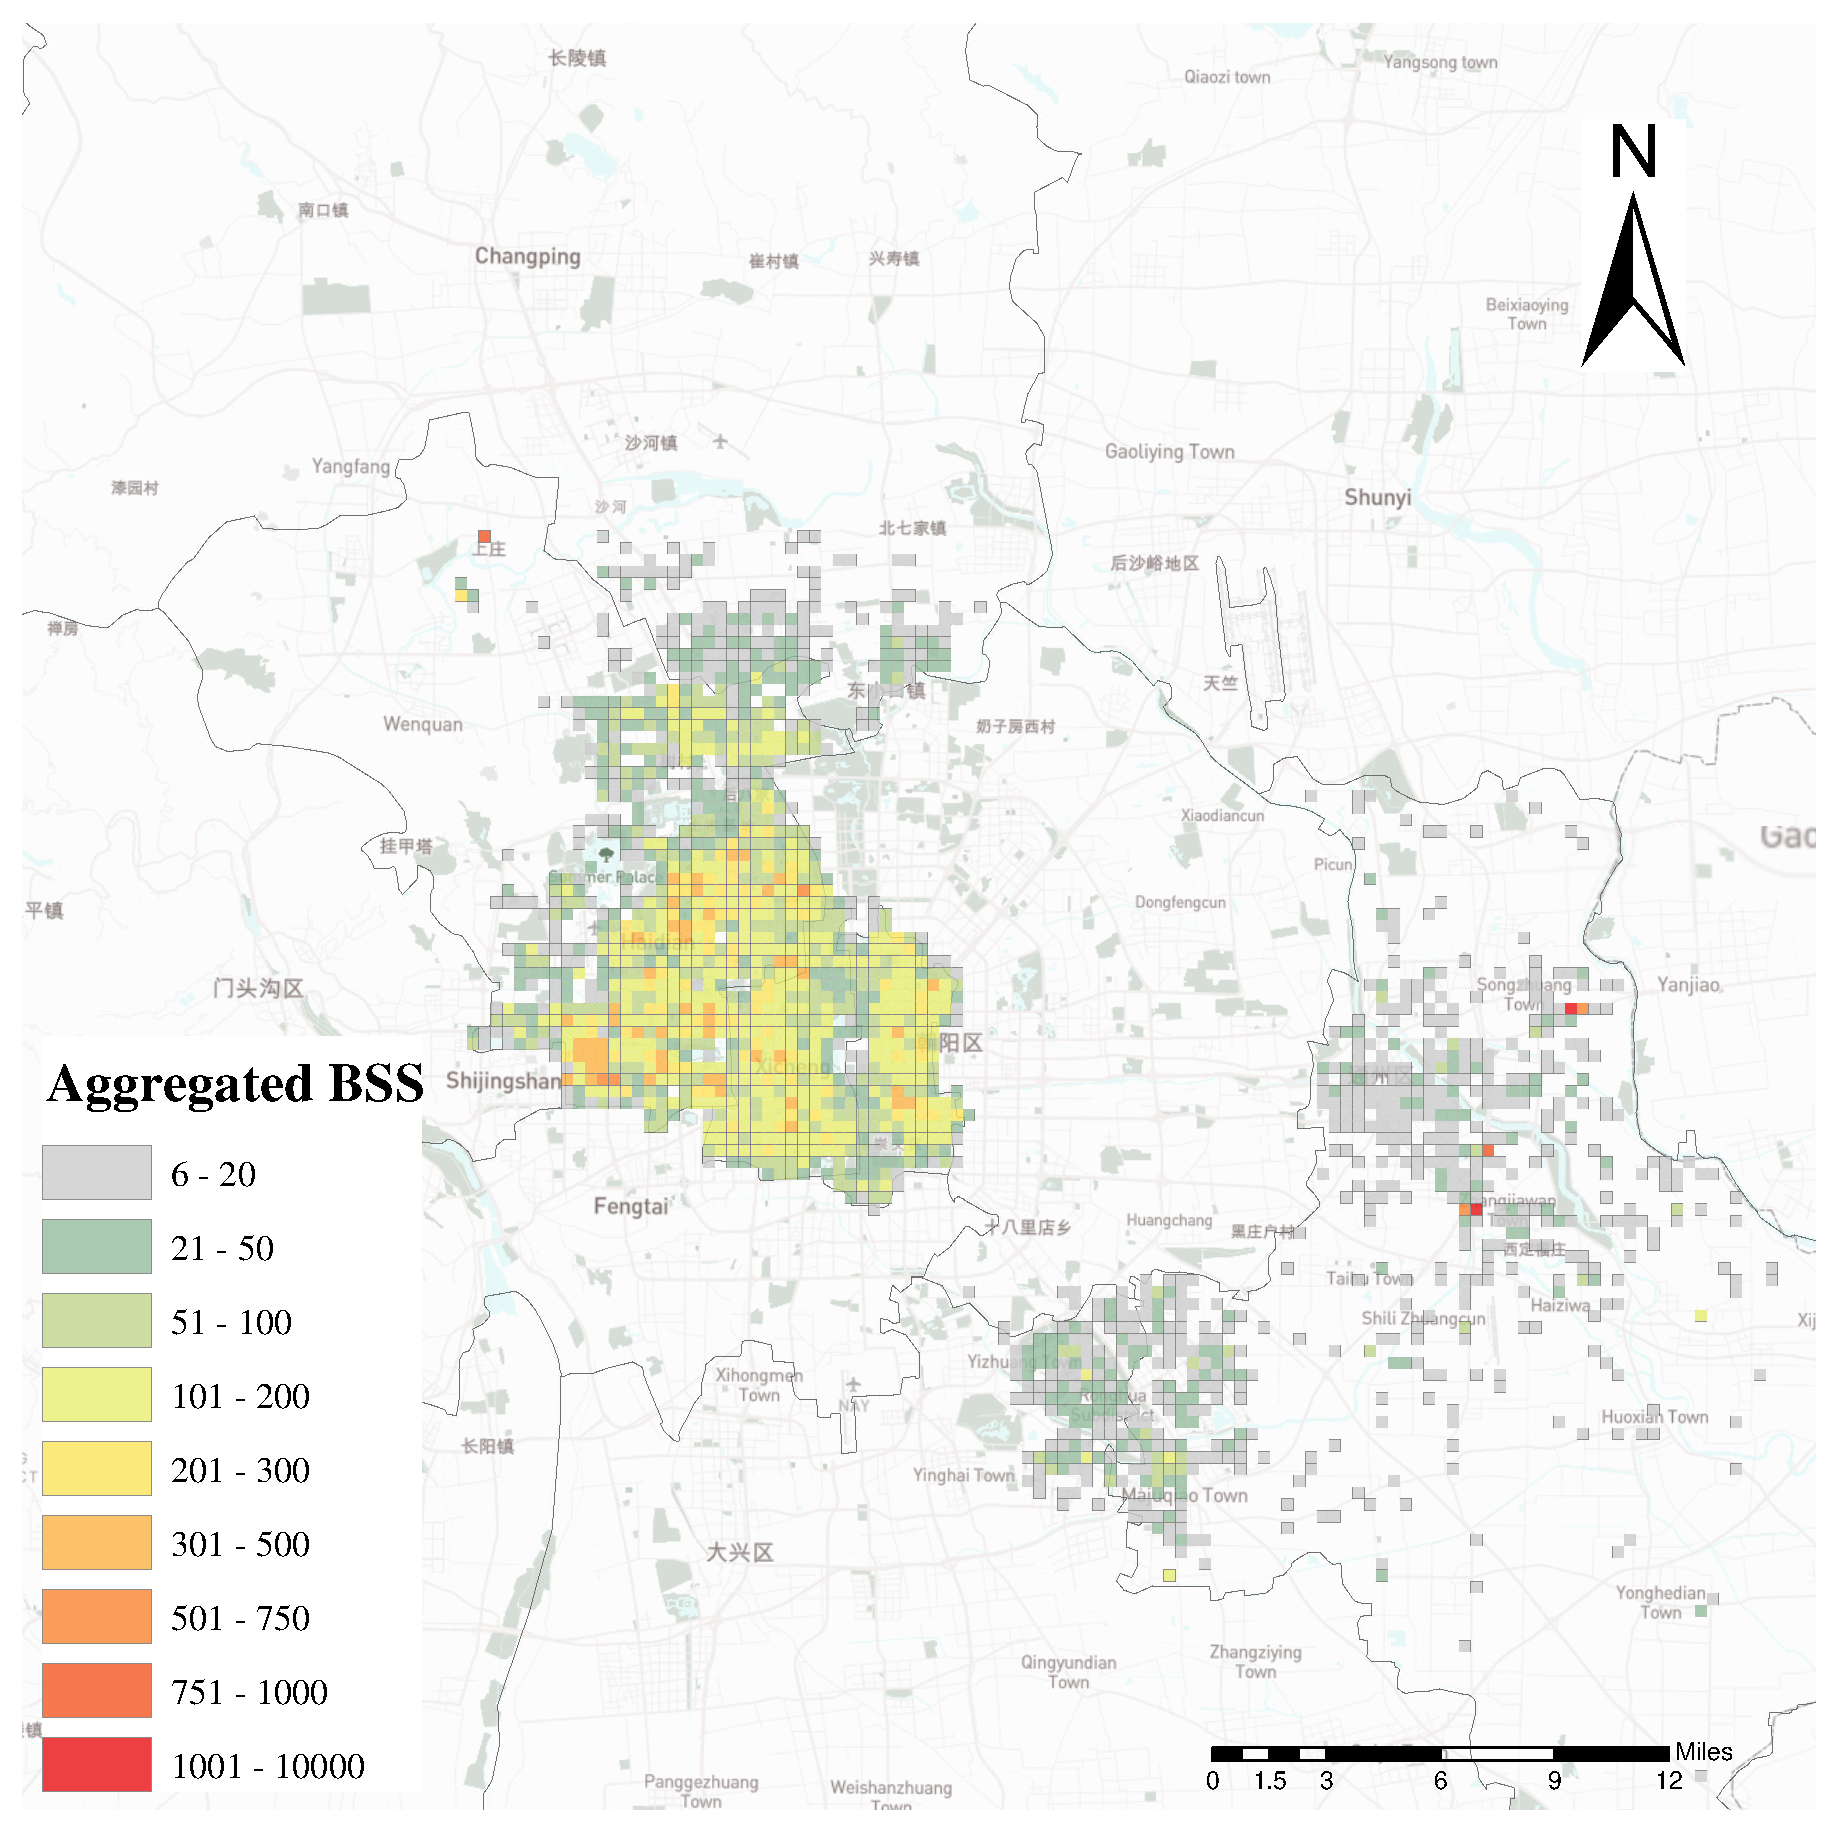
\includegraphics[width=\textwidth]{Figures/BSSPhase3_2020.eps}
        \caption{After spring festival 2020}
    \end{subfigure}
    
    \vspace{6pt}
    \begin{subfigure}{.3\textwidth}
        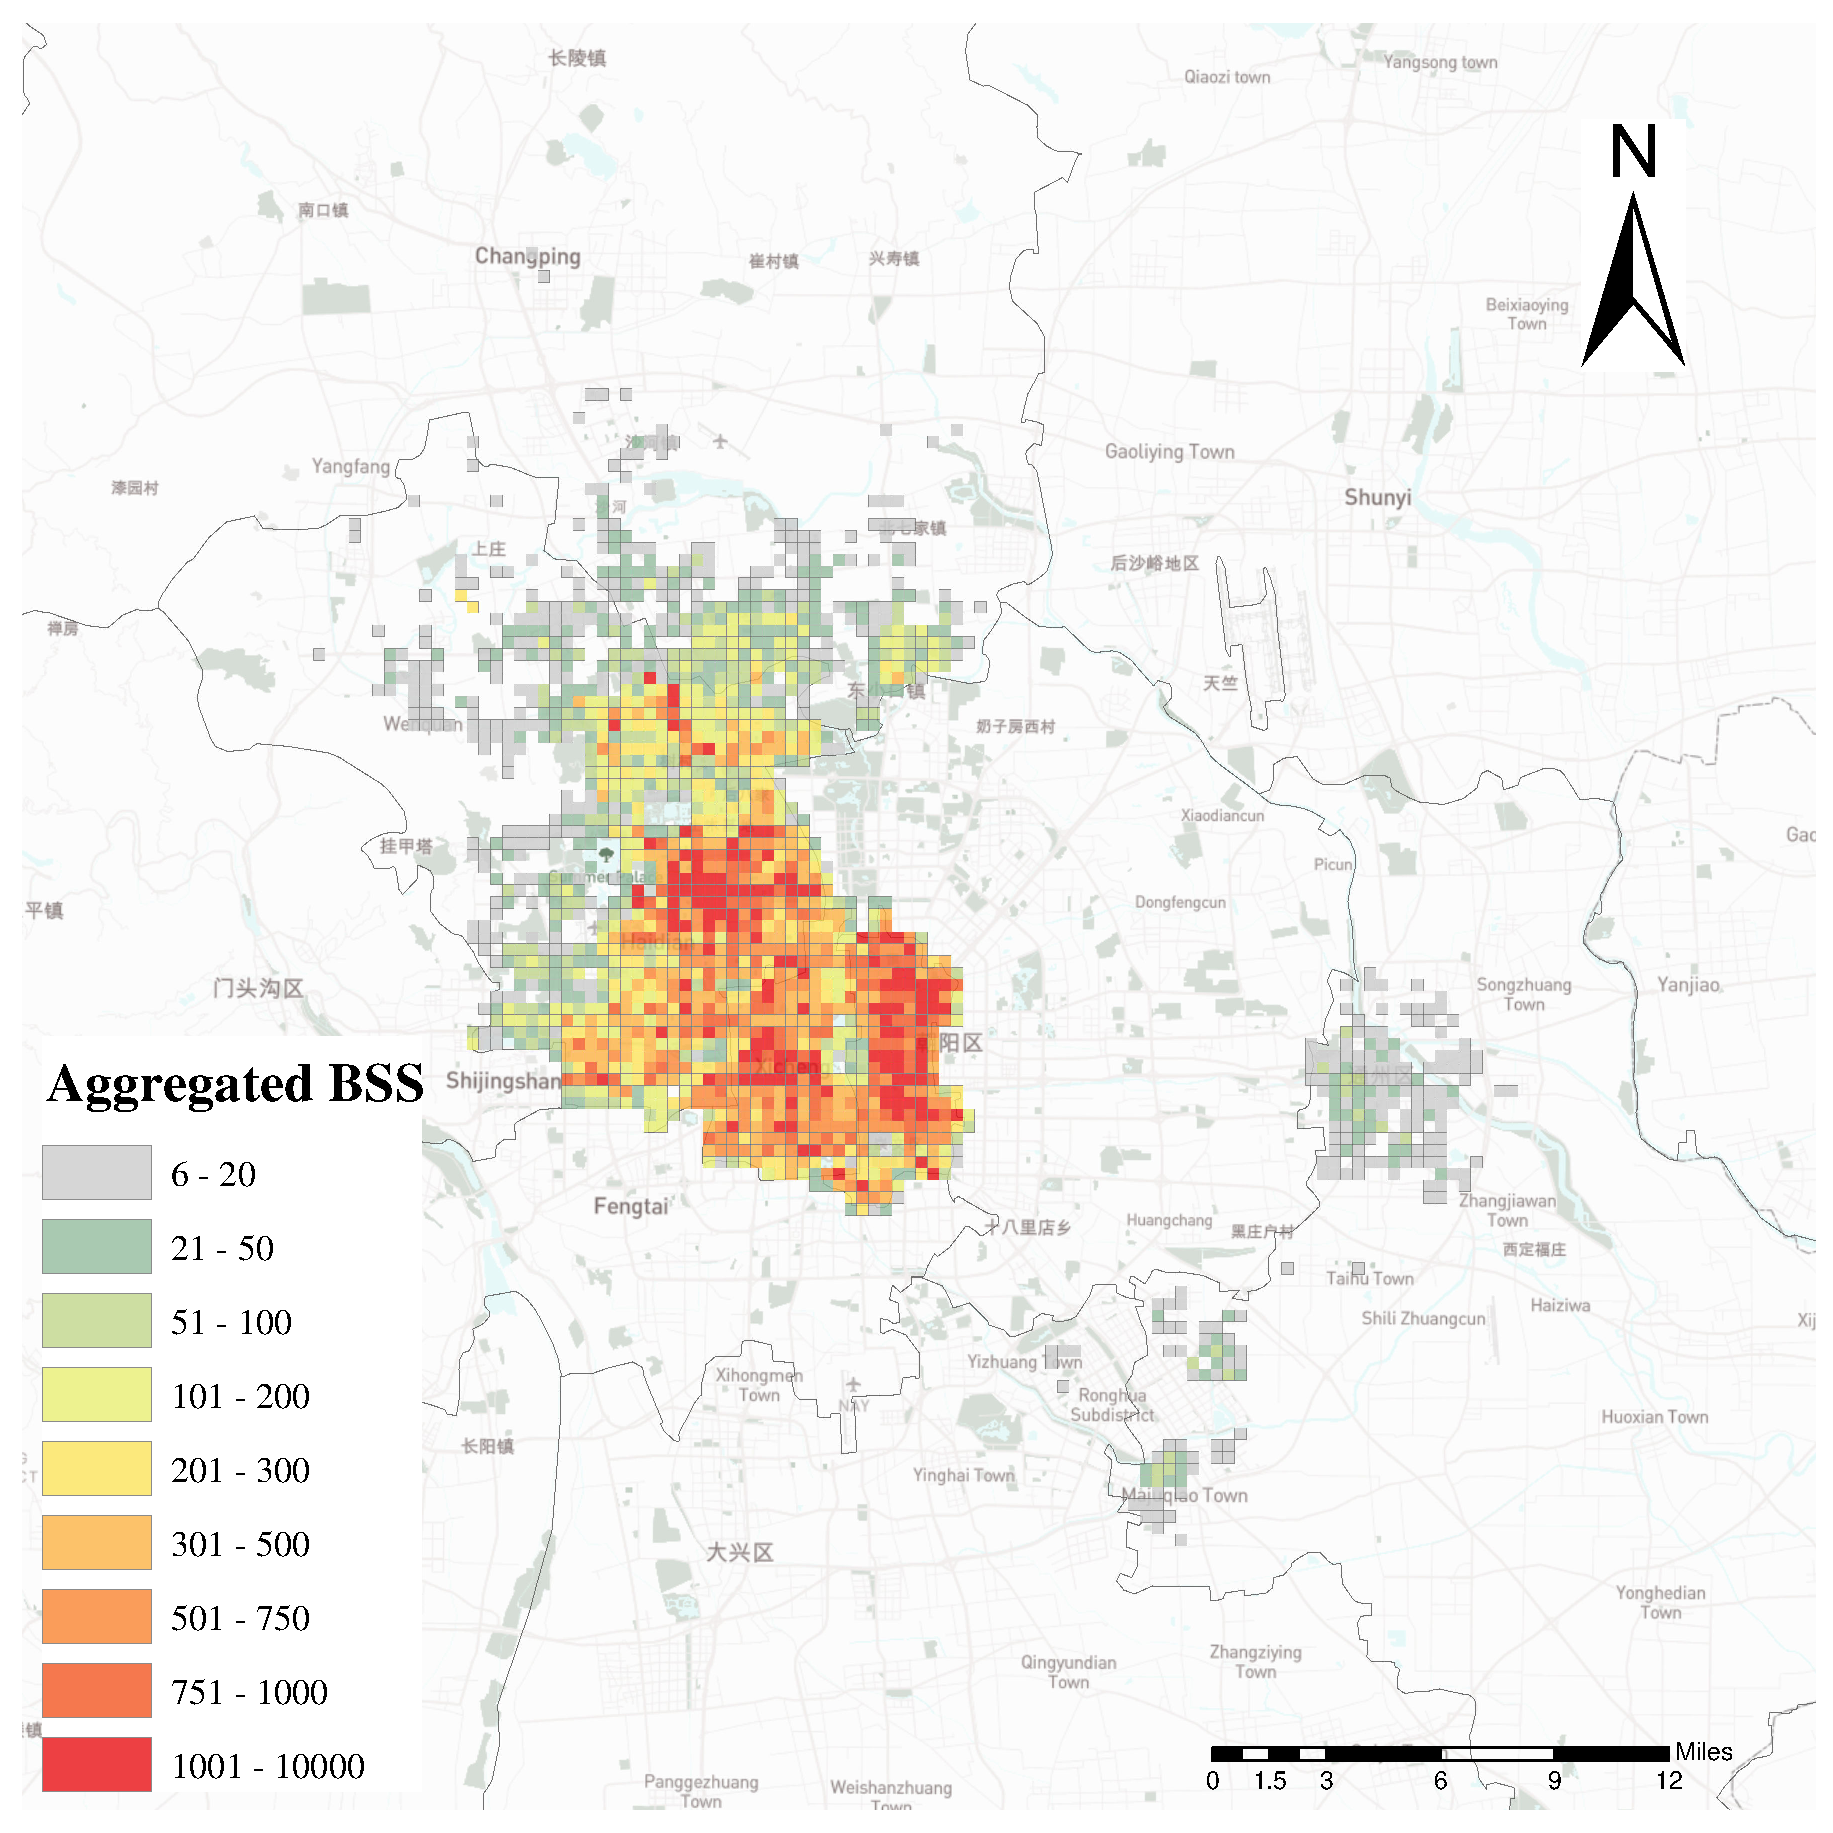
\includegraphics[width=\textwidth]{Figures/BSSPhase1_2019.eps}
        \caption{Before spring festival 2019}
    \end{subfigure}
    \begin{subfigure}{.3\textwidth}
        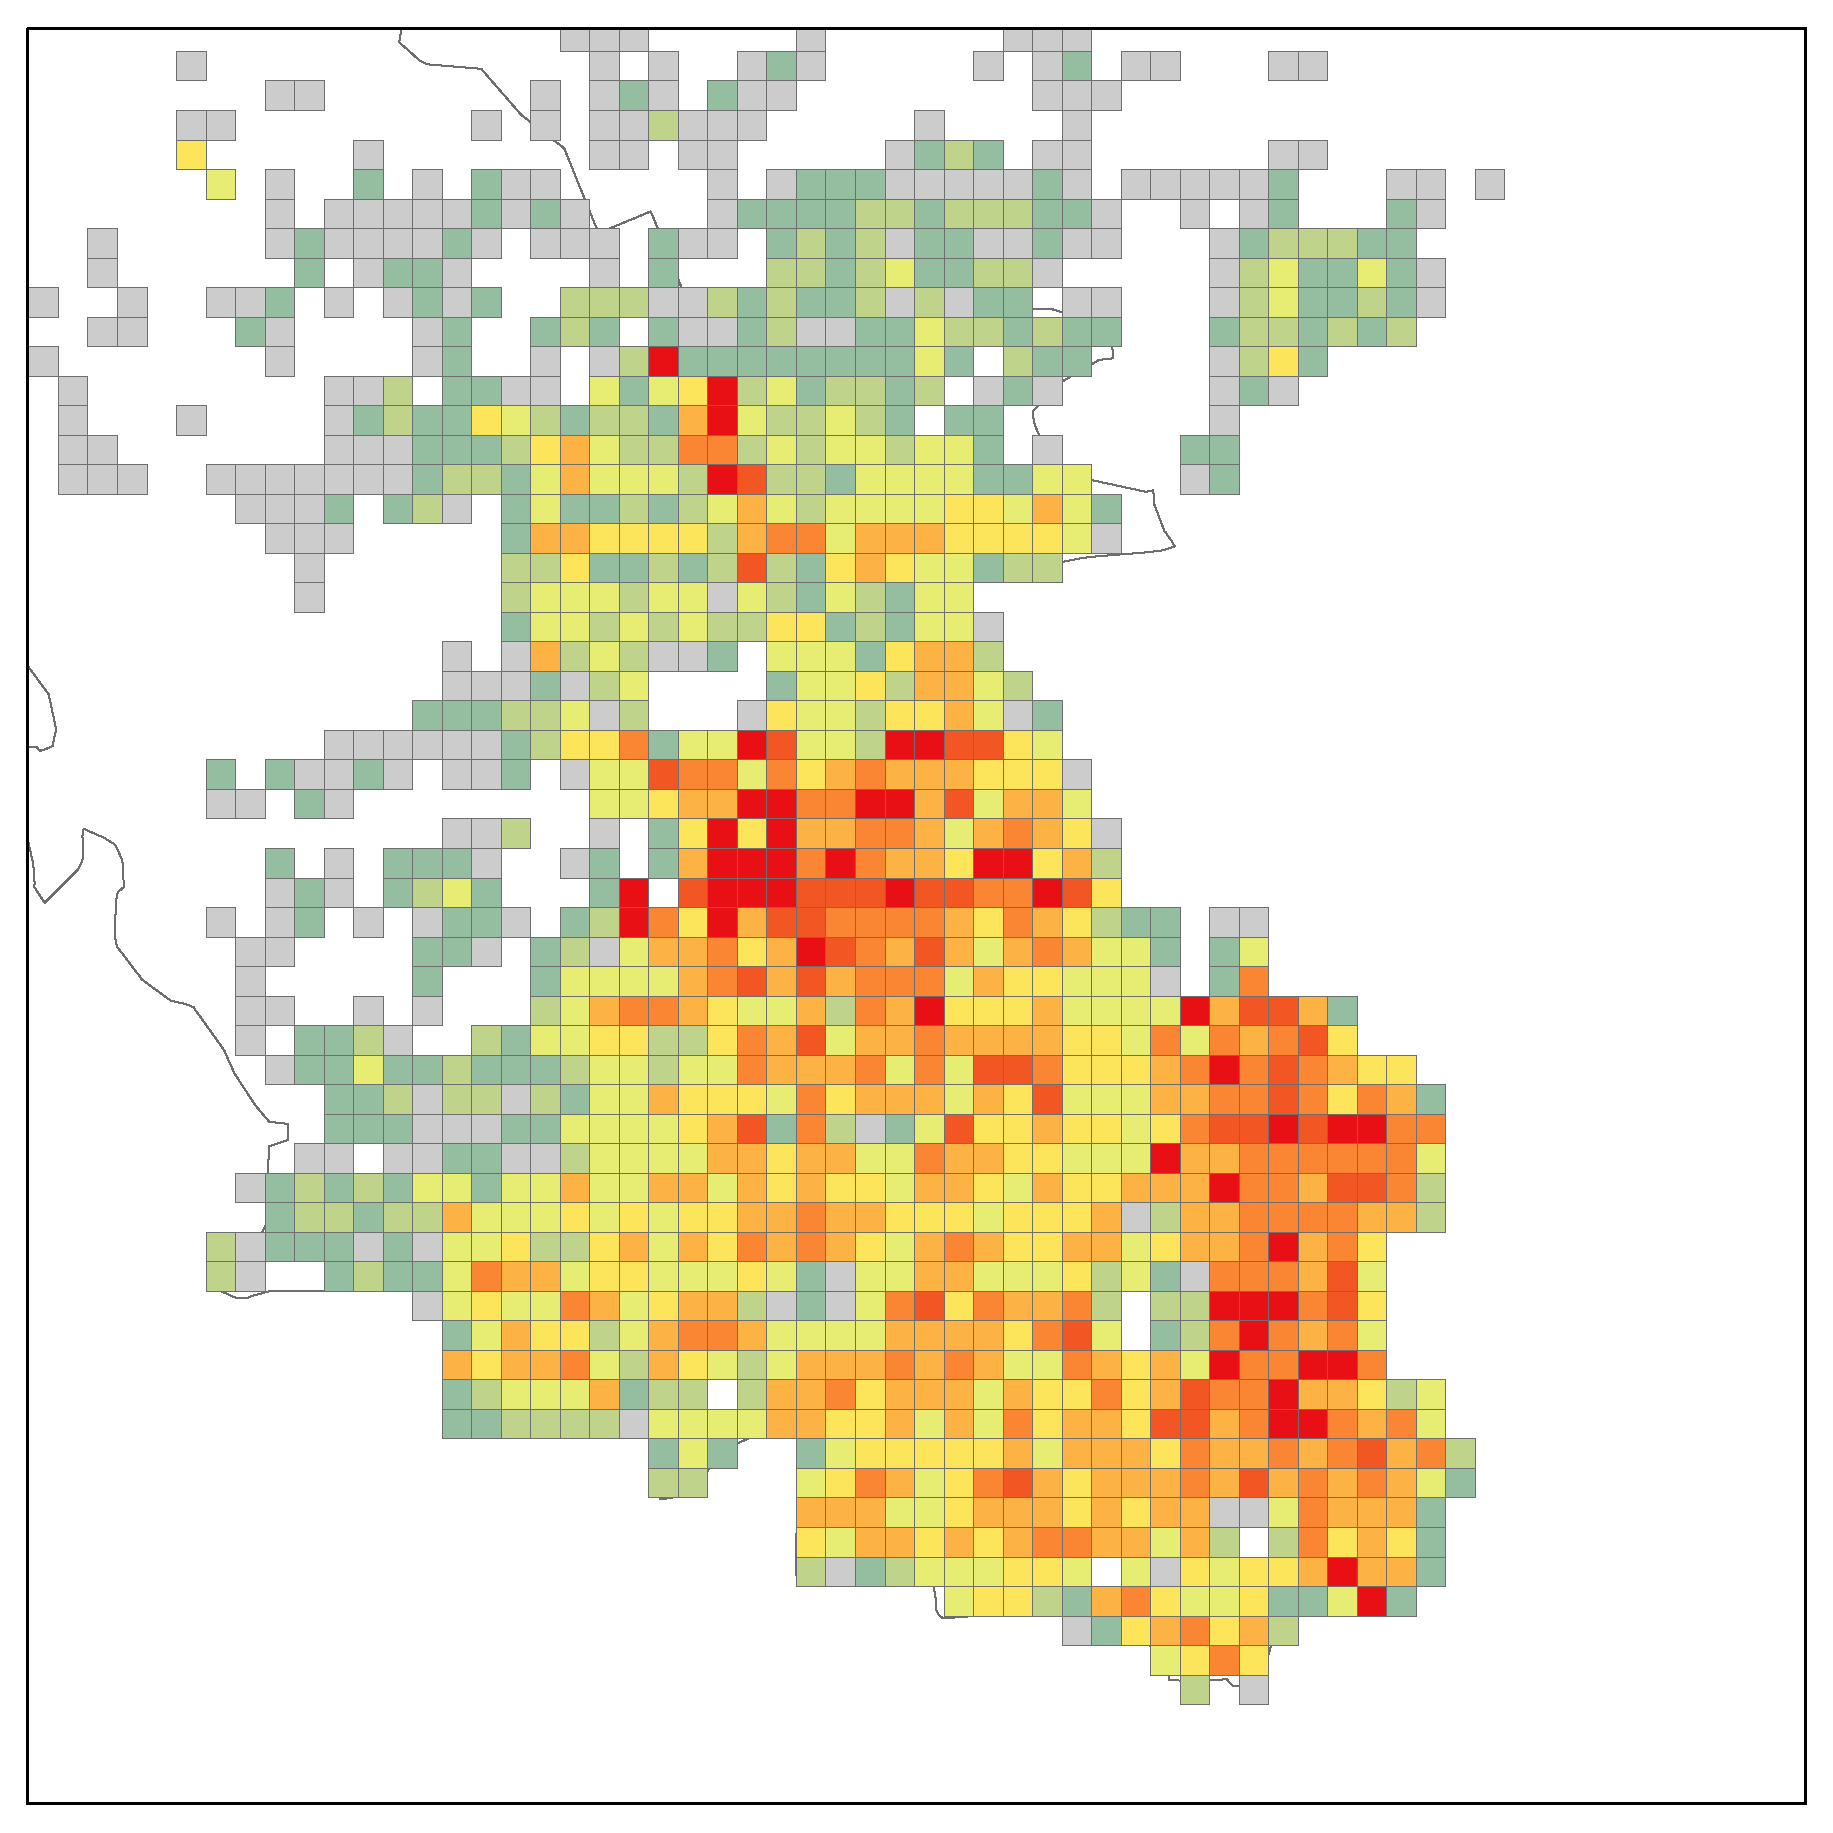
\includegraphics[width=\textwidth]{Figures/BSSPhase2_2019.eps}
        \caption{Spring festival 2019}
    \end{subfigure}
    \begin{subfigure}{.3\textwidth}
        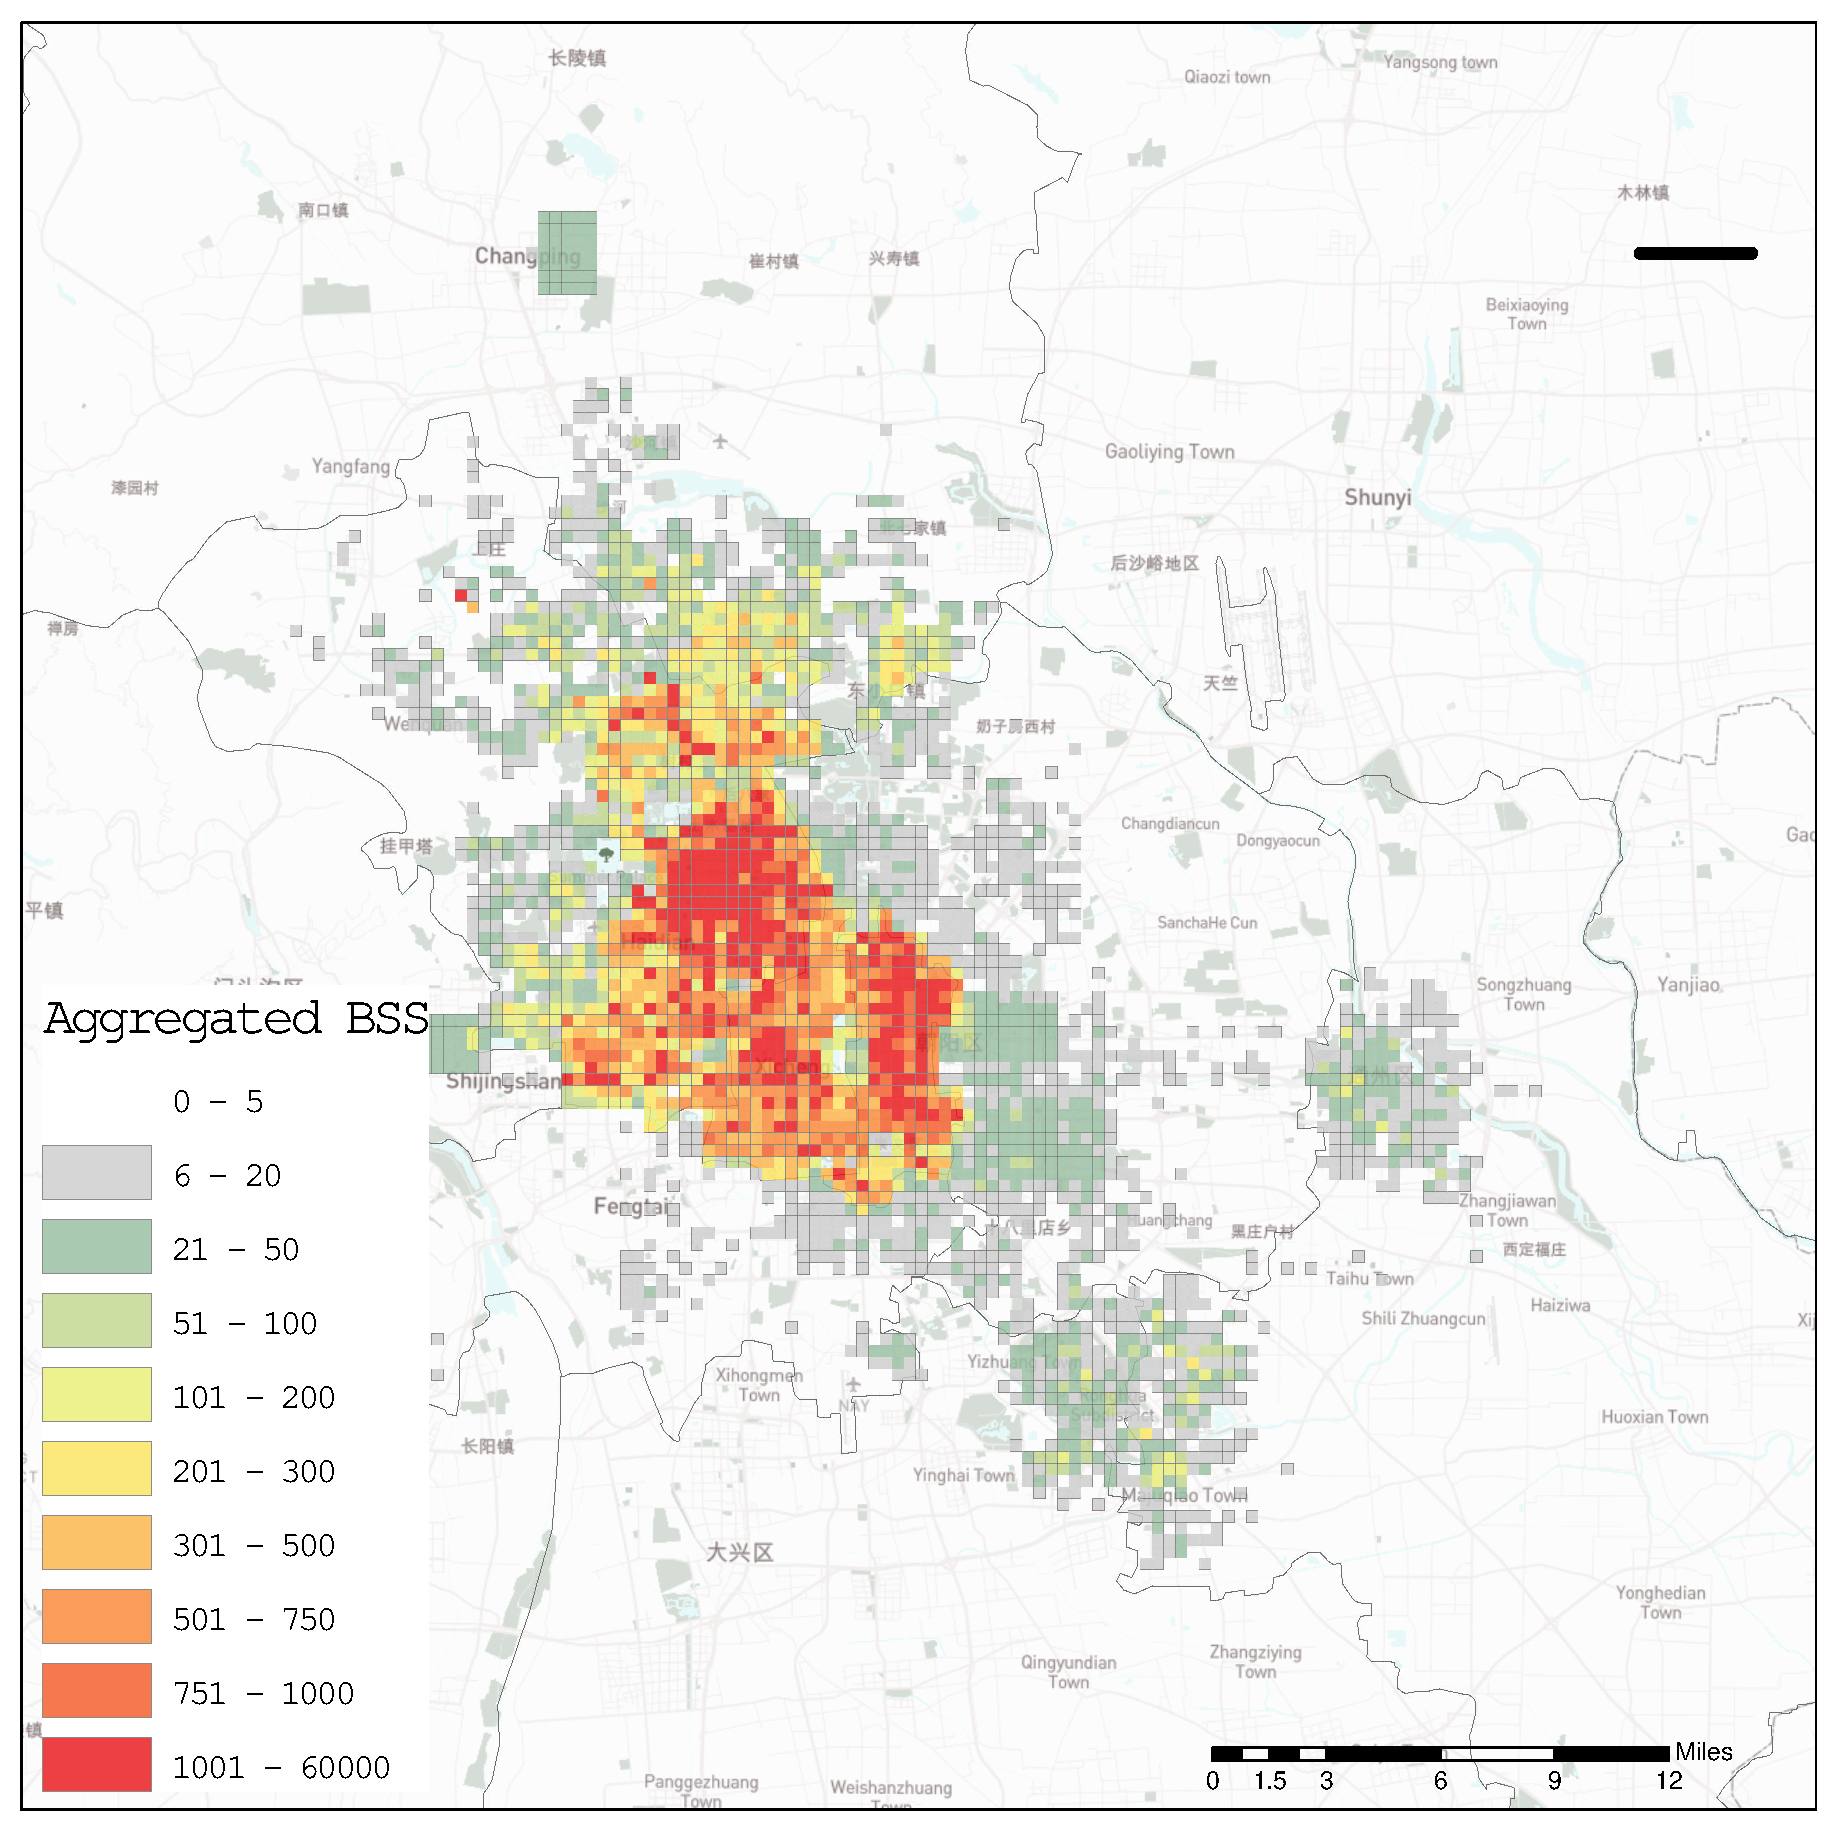
\includegraphics[width=\textwidth]{Figures/BSSPhase3_2019.eps}
        \caption{After spring festival 2019}
    \end{subfigure}
    
    \vspace{6pt}
    \begin{subfigure}{.3\textwidth}
        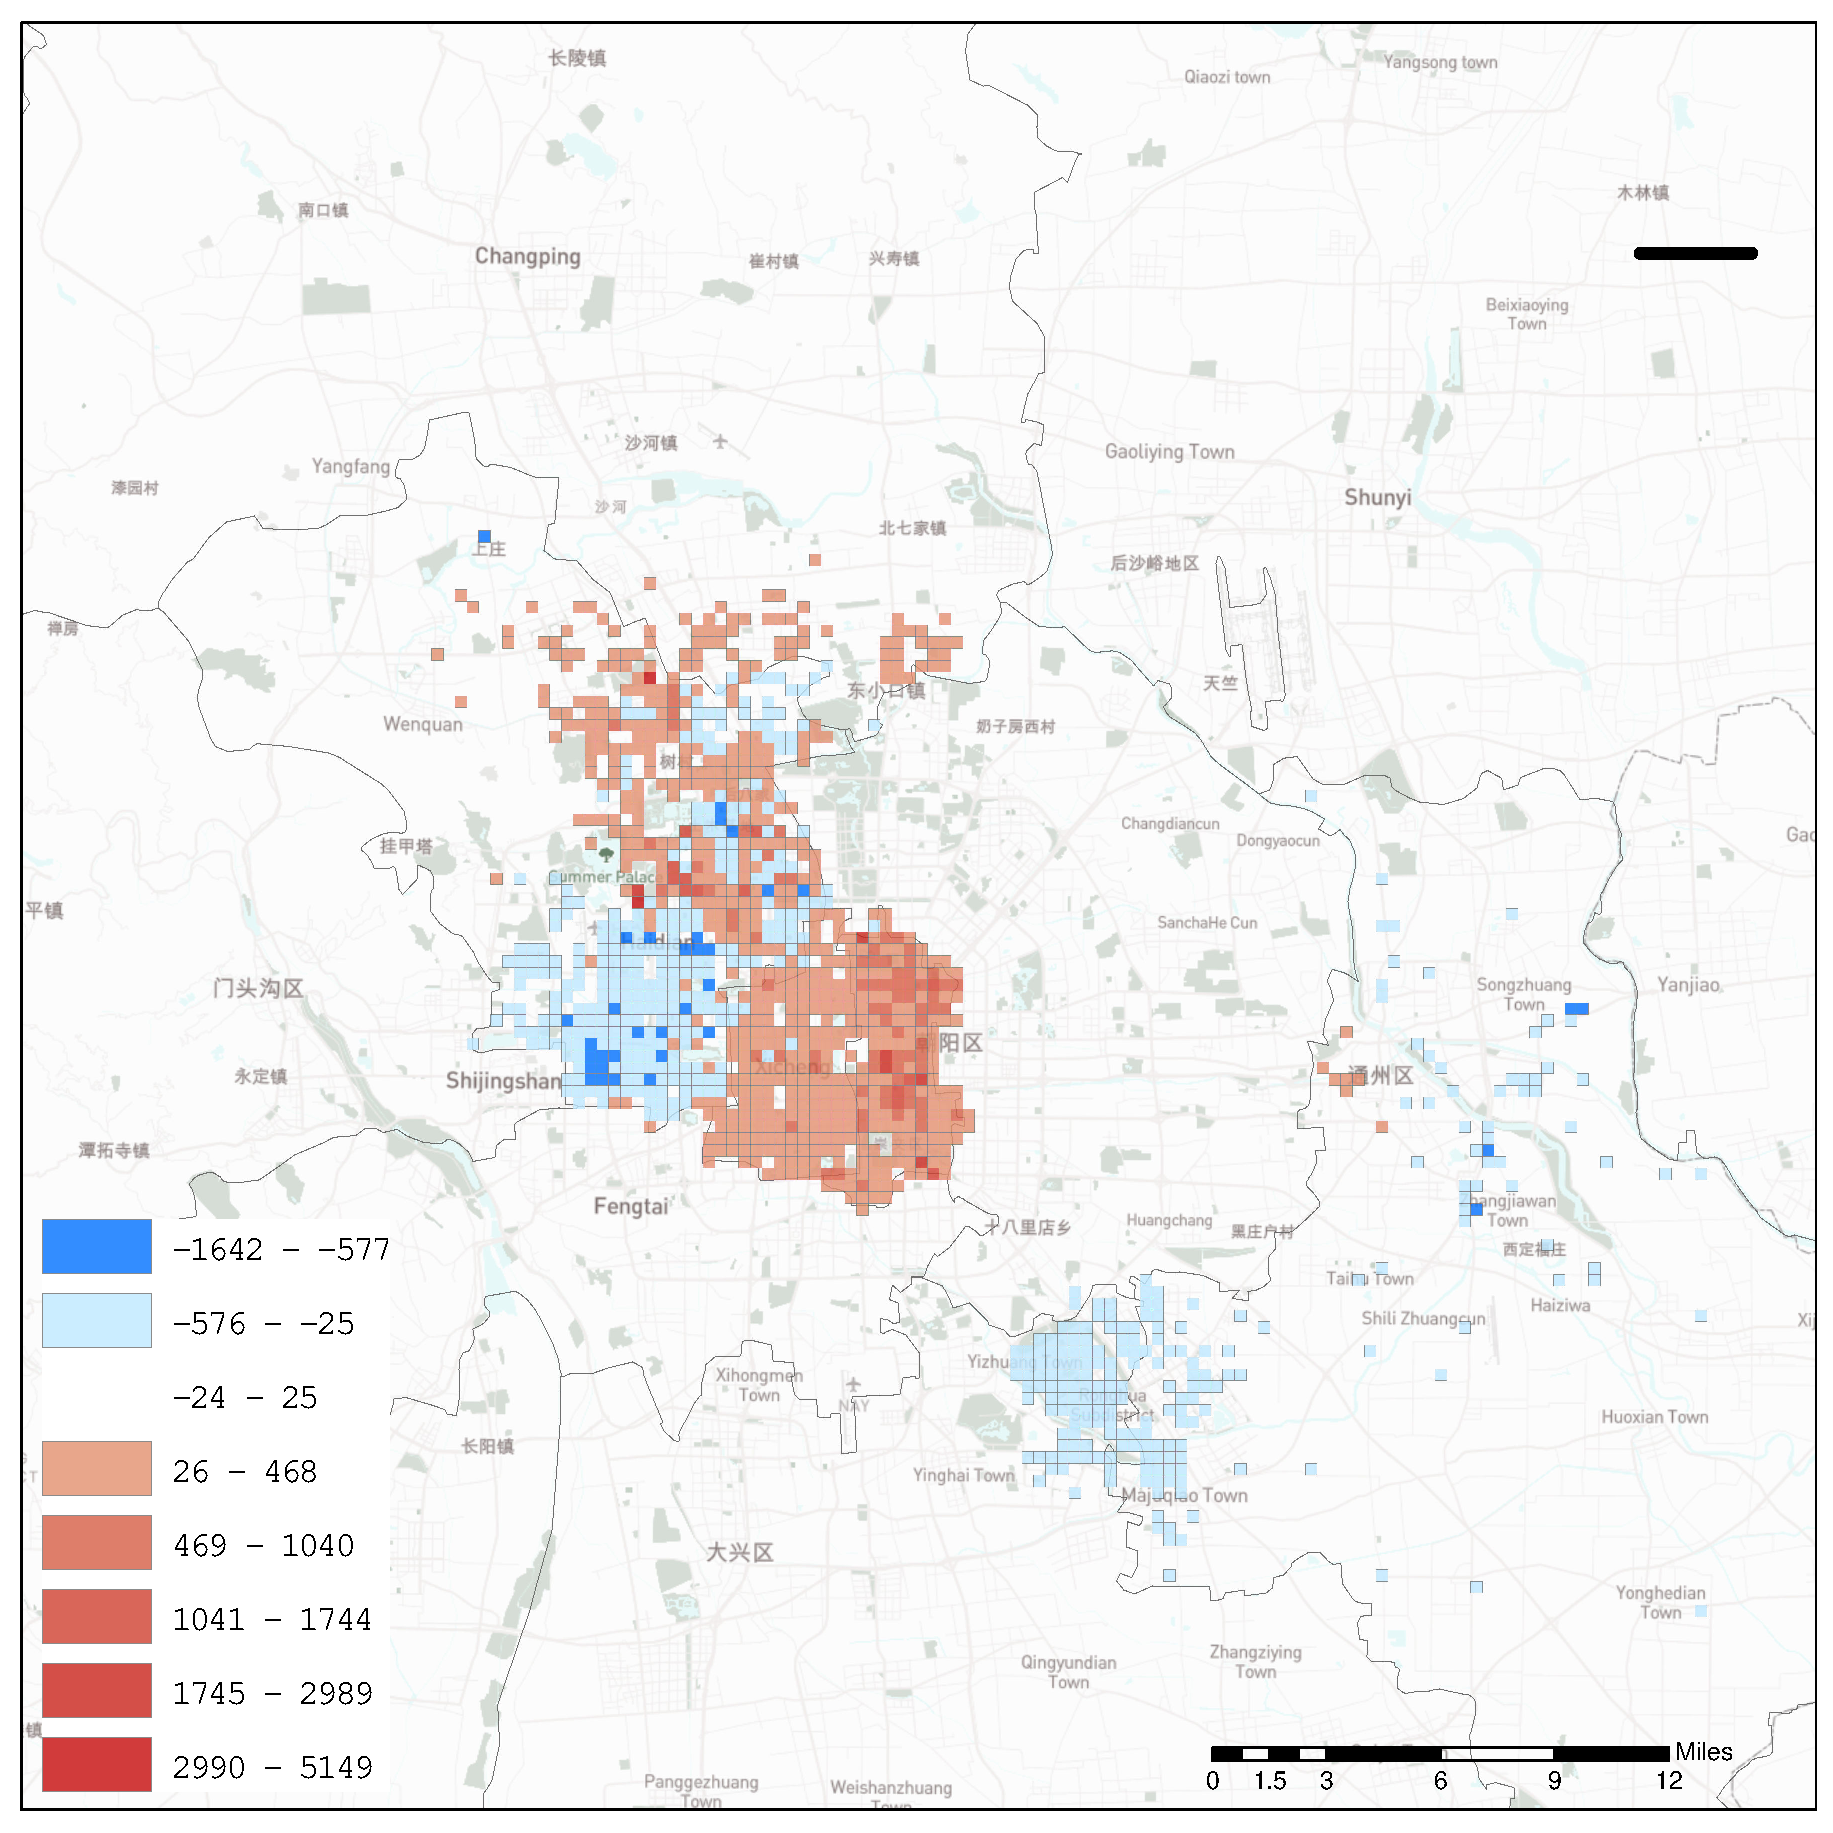
\includegraphics[width=\textwidth]{Figures/BSSMinusmp1.eps}
        \caption{Differential image of Phase 1}
    \end{subfigure}
        \begin{subfigure}{.3\textwidth}
        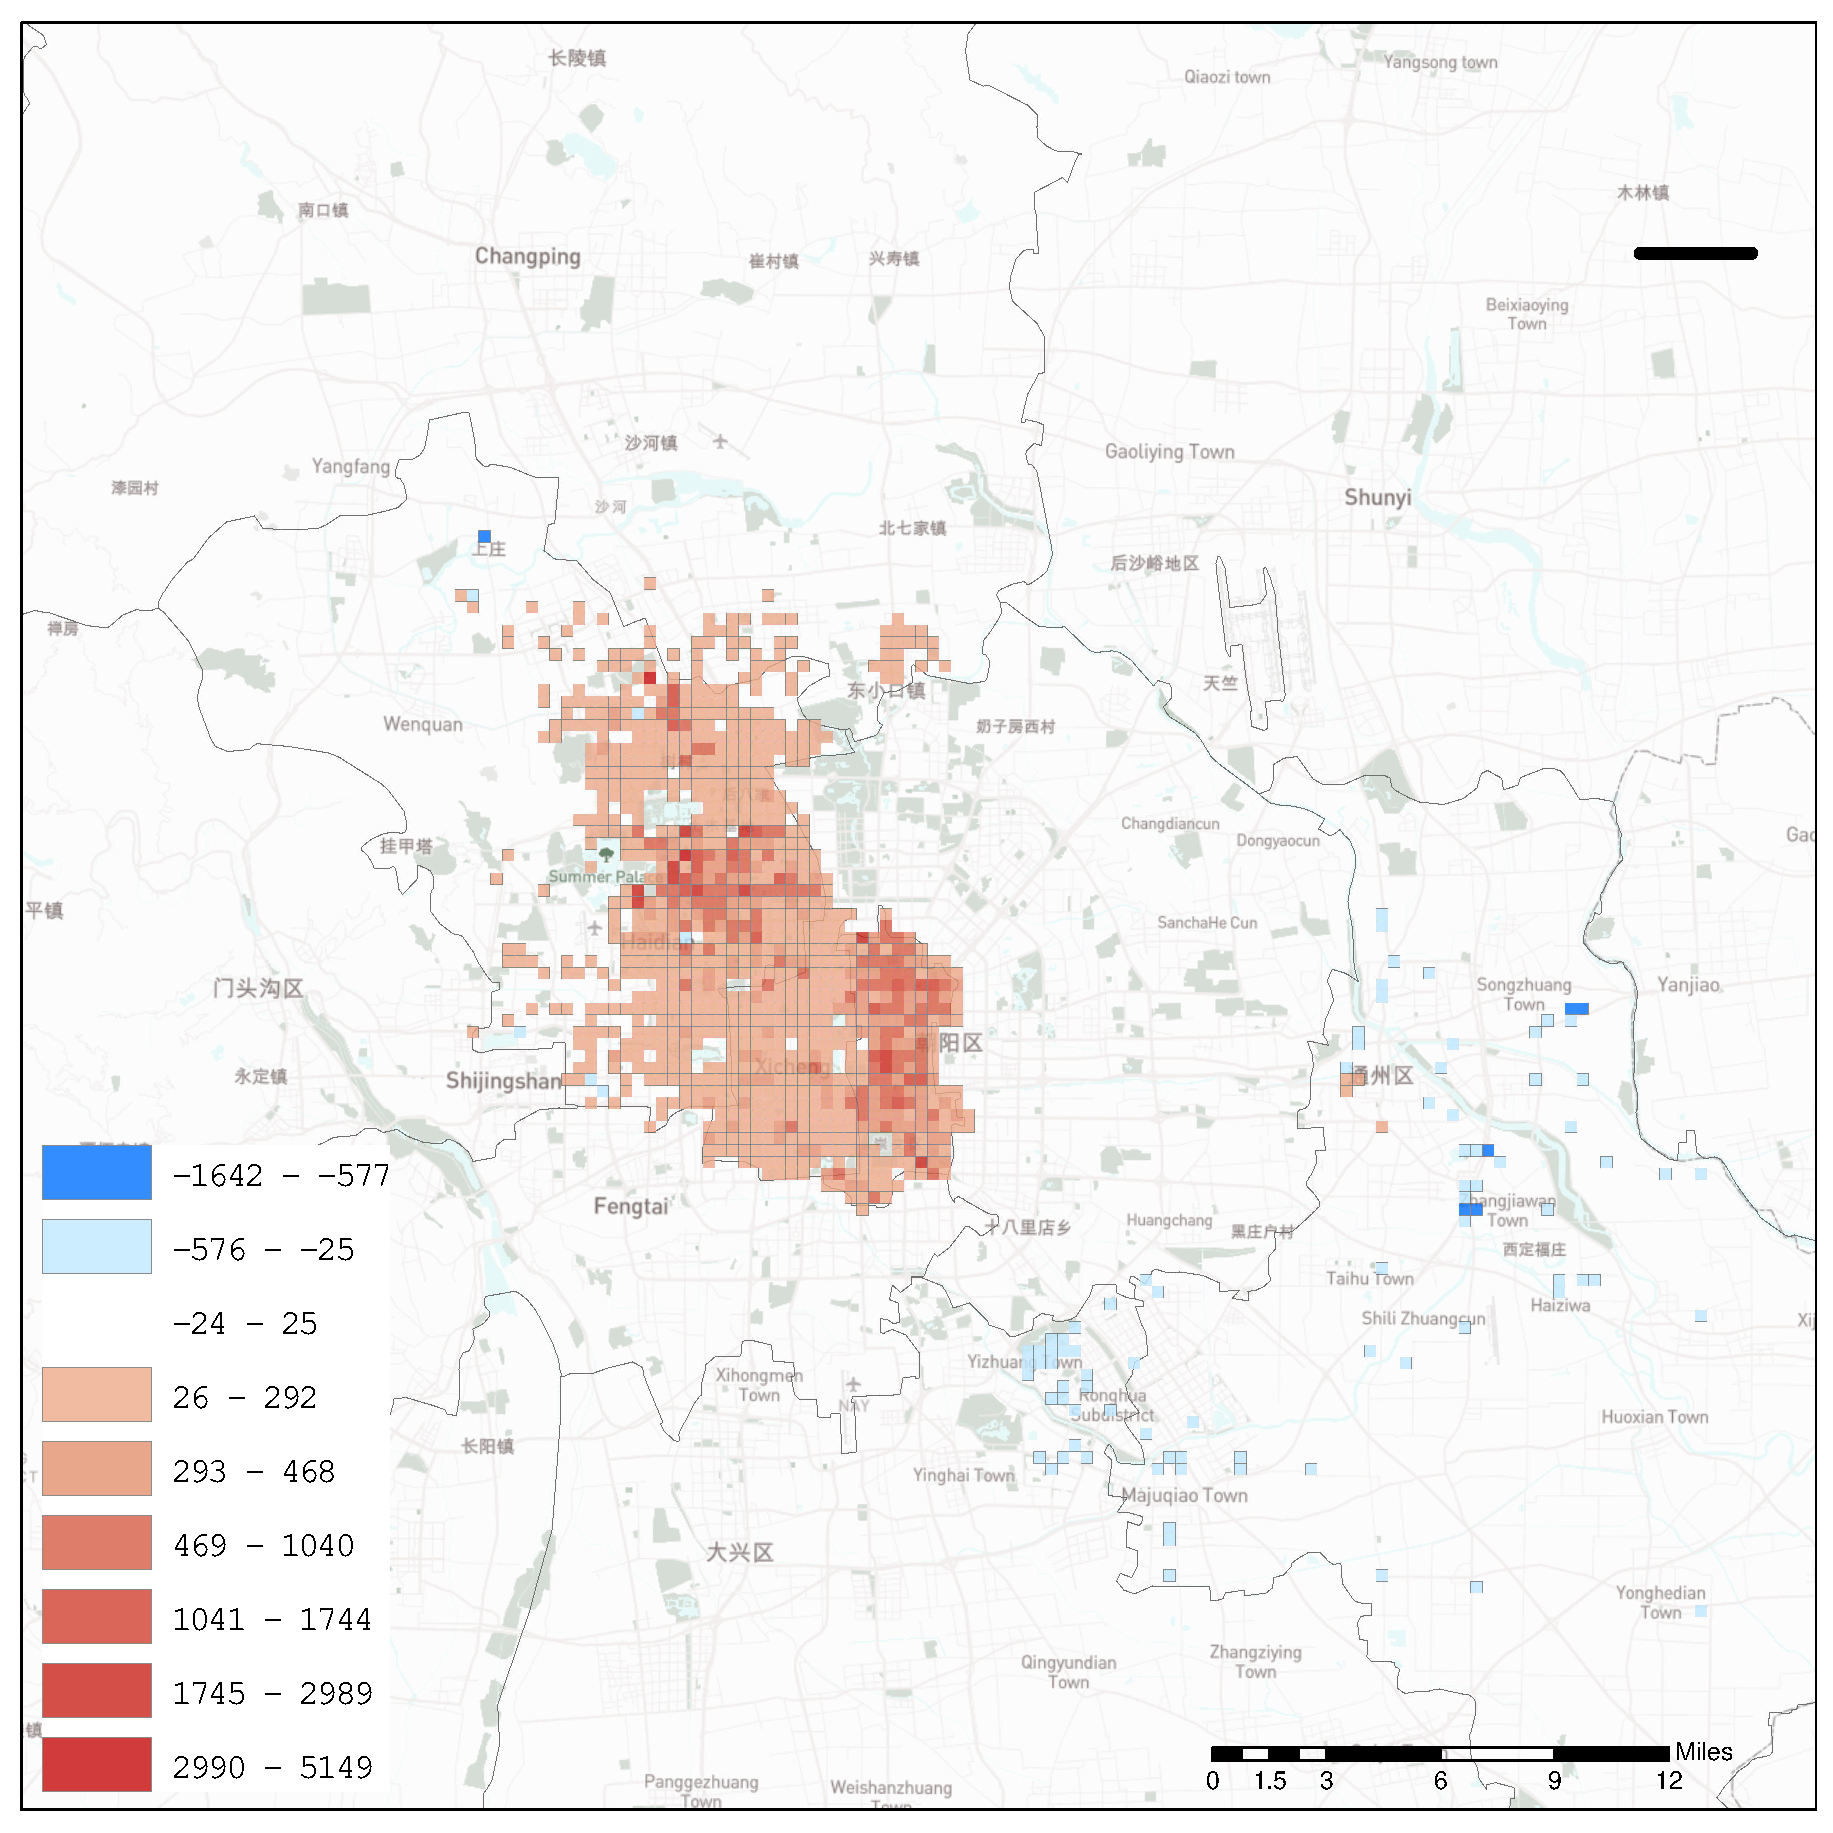
\includegraphics[width=\textwidth]{Figures/BSSMinusmp2.eps}
        \caption{Differential image of Phase 2}
    \end{subfigure}
        \begin{subfigure}{.3\textwidth}
        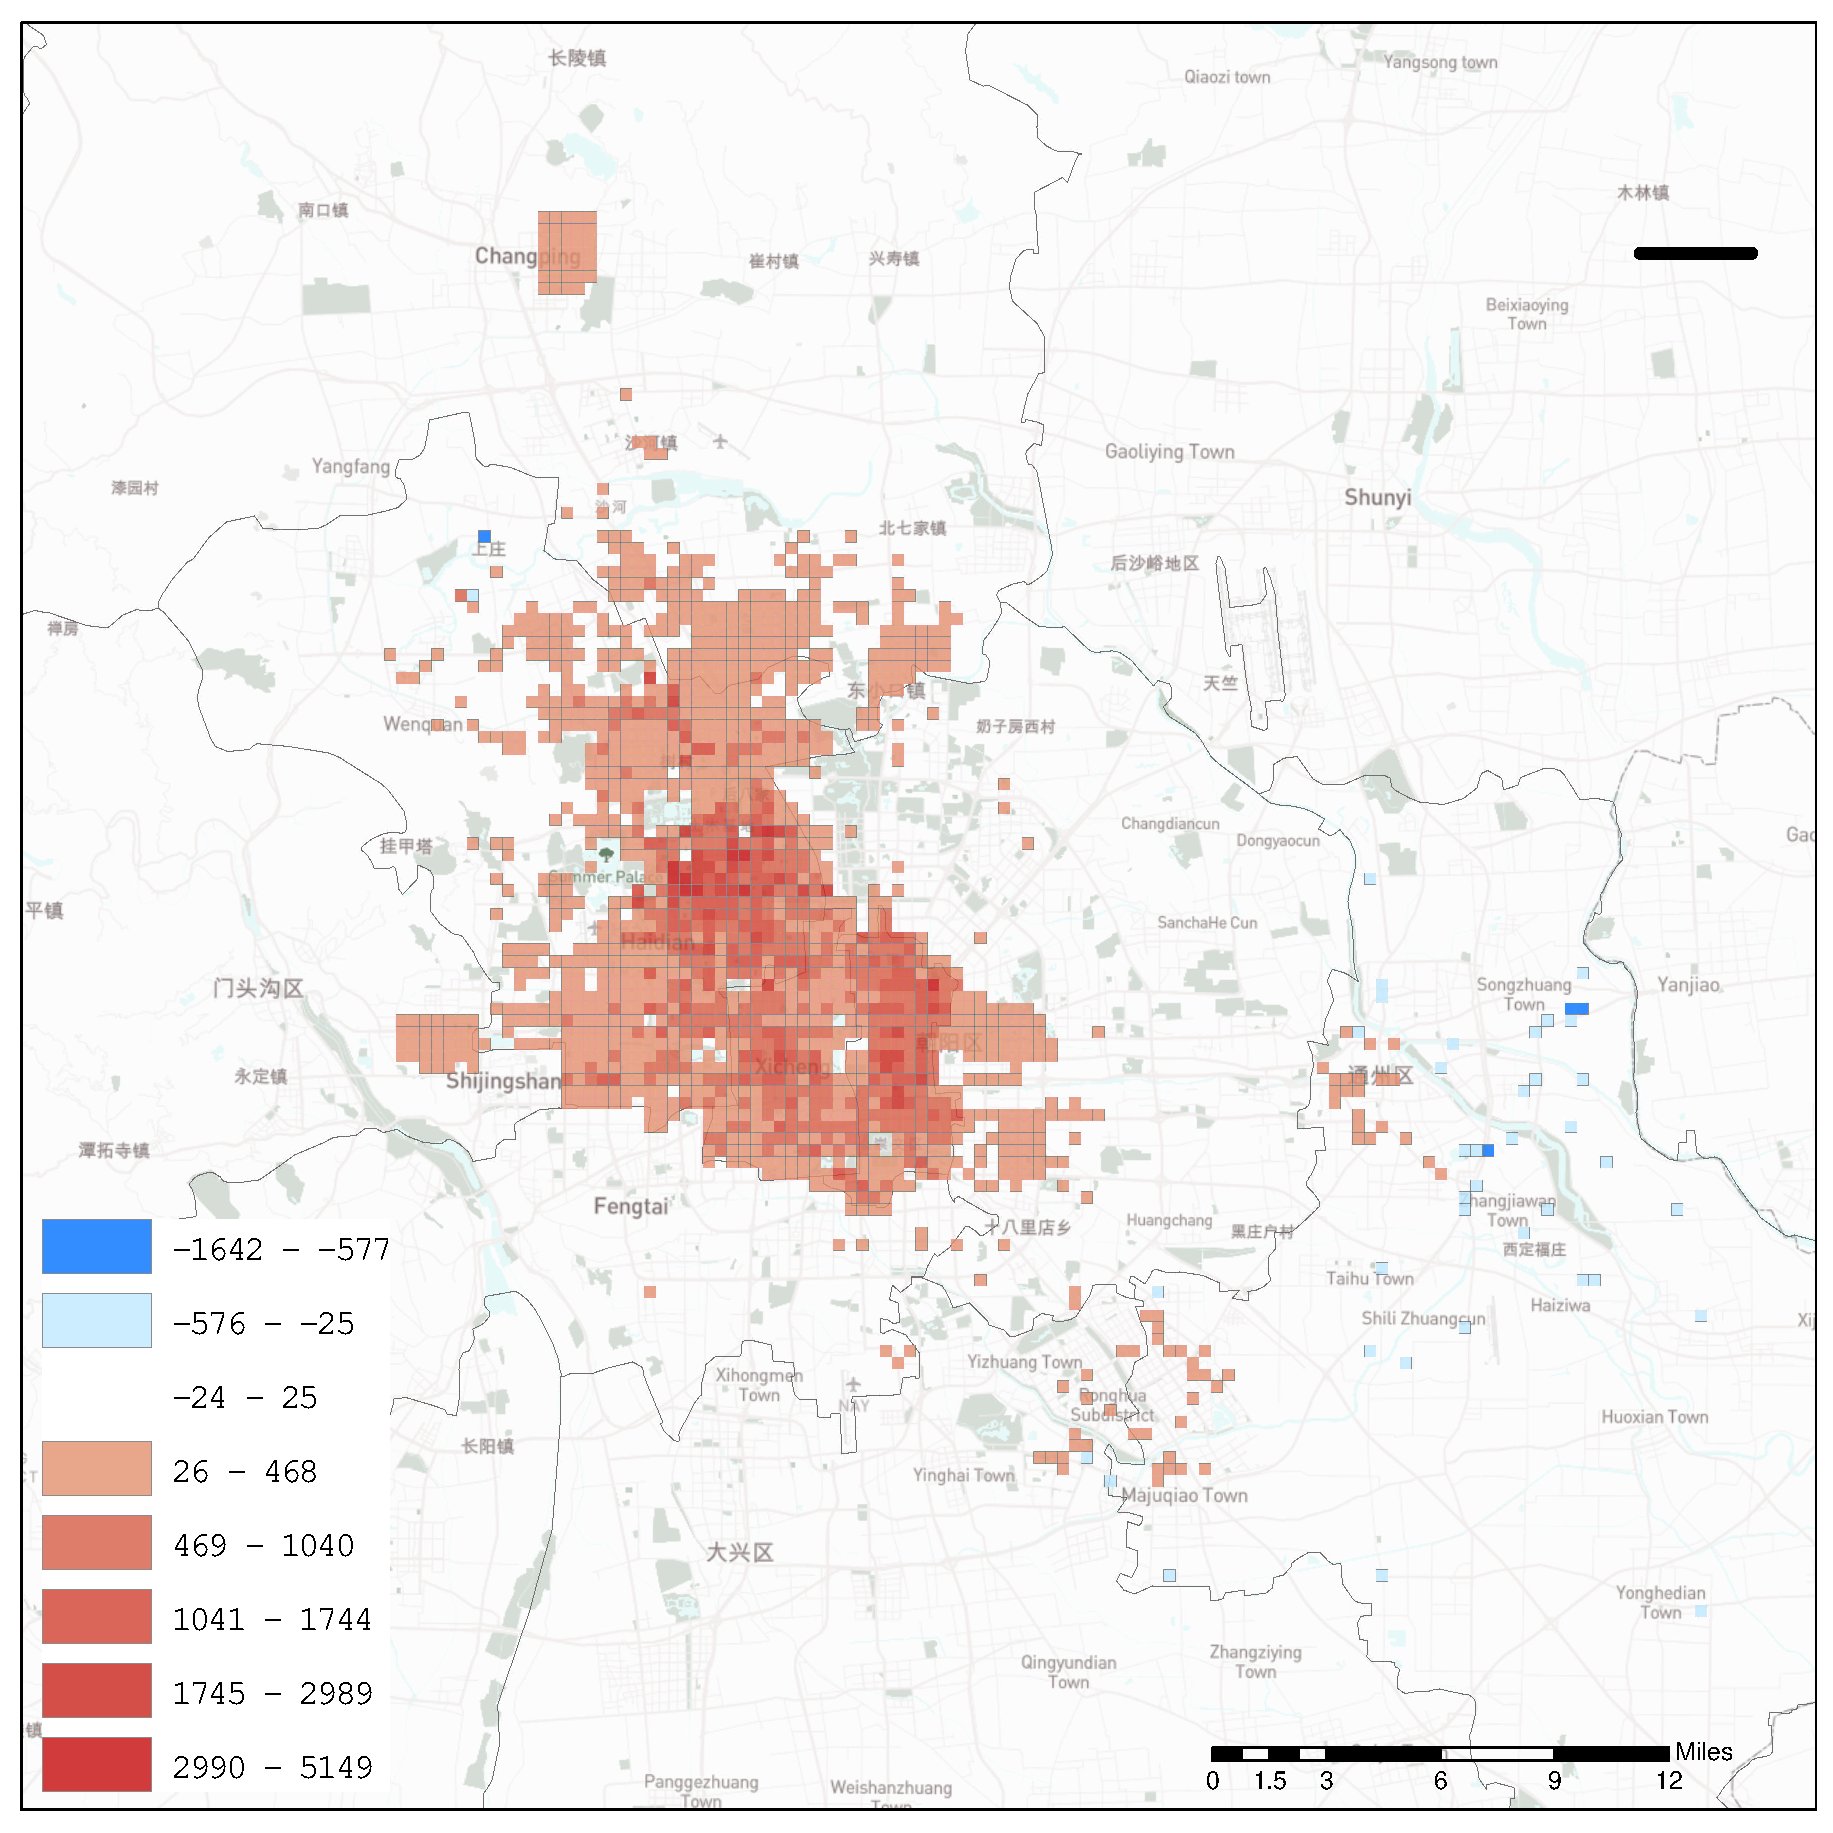
\includegraphics[width=\textwidth]{Figures/BSSMinusmp3.eps}
        \caption{Differential image of Phase 3}
    \end{subfigure}
    \caption{Caption}
    \label{fig:compare_2019_and_2020}
\end{figure}

Overall visualization of different periods (before Chinese New Year, during the quarantine period, epidemics mitigated)

%%%%%%%%%%%%%%%%%%%%%%%%%%%%%%%%%%%%%%%%%%
Part 2. Relationships between cycling activities and confirmed cases with respect to epidemic phases
\textcolor{red}{During the epidemic control, cycling activities reduced while the confirmed cases increased, which can be inferred from visual interpretation.}
\begin{figure}[H]
    \centering
    \begin{subfigure}{.3\textwidth}
        \includegraphics[width=\textwidth]{Figures/Relation_with_confrimed_cases/NewDistrictSSBD2020_01_21.eps}
        \caption{21 Jan}
    \end{subfigure}
    \begin{subfigure}{.3\textwidth}
        \includegraphics[width=\textwidth]{Figures/Relation_with_confrimed_cases/NewDistrictSSBD2020_01_25.eps}
        \caption{25 Jan}
    \end{subfigure}
    \begin{subfigure}{.3\textwidth}
        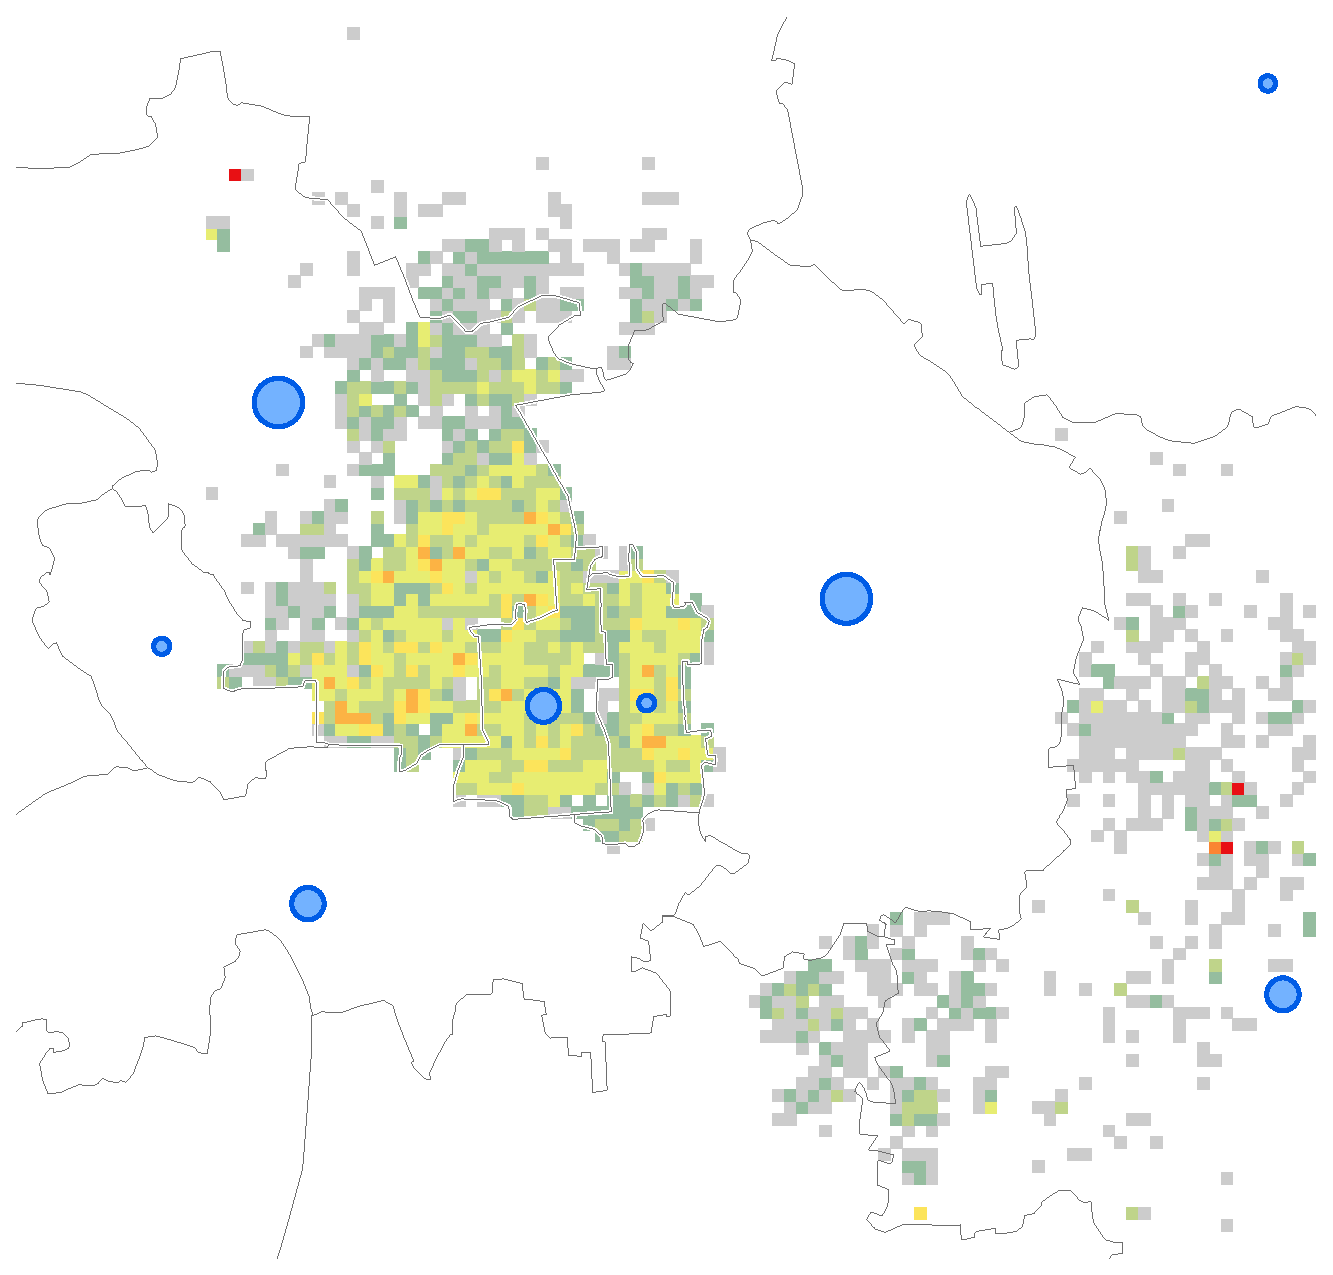
\includegraphics[width=\textwidth]{Figures/Relation_with_confrimed_cases/NewDistrictSSBD2020_01_30.eps}
        \caption{30 Jan}
    \end{subfigure}

    \vspace{6pt}    
    \begin{subfigure}{.3\textwidth}
        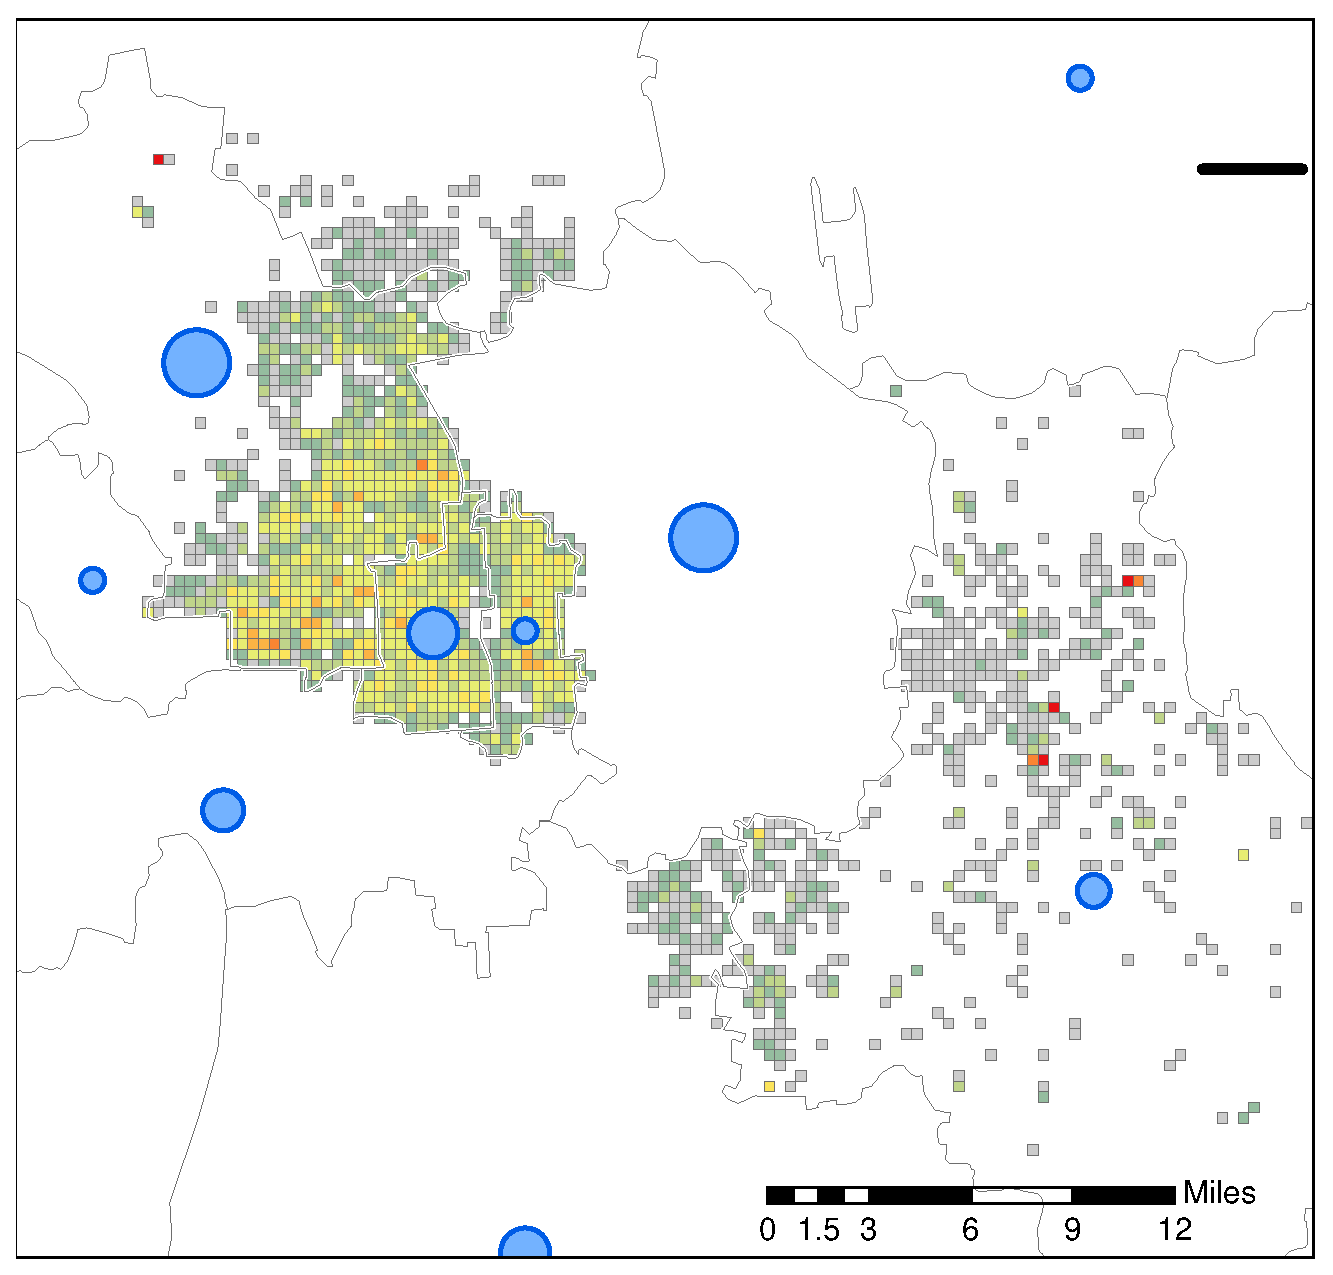
\includegraphics[width=\textwidth]{Figures/Relation_with_confrimed_cases/NewDistrictSSBD2020_02_04.eps}
        \caption{04 Feb}
    \end{subfigure}
    \begin{subfigure}{.3\textwidth}
        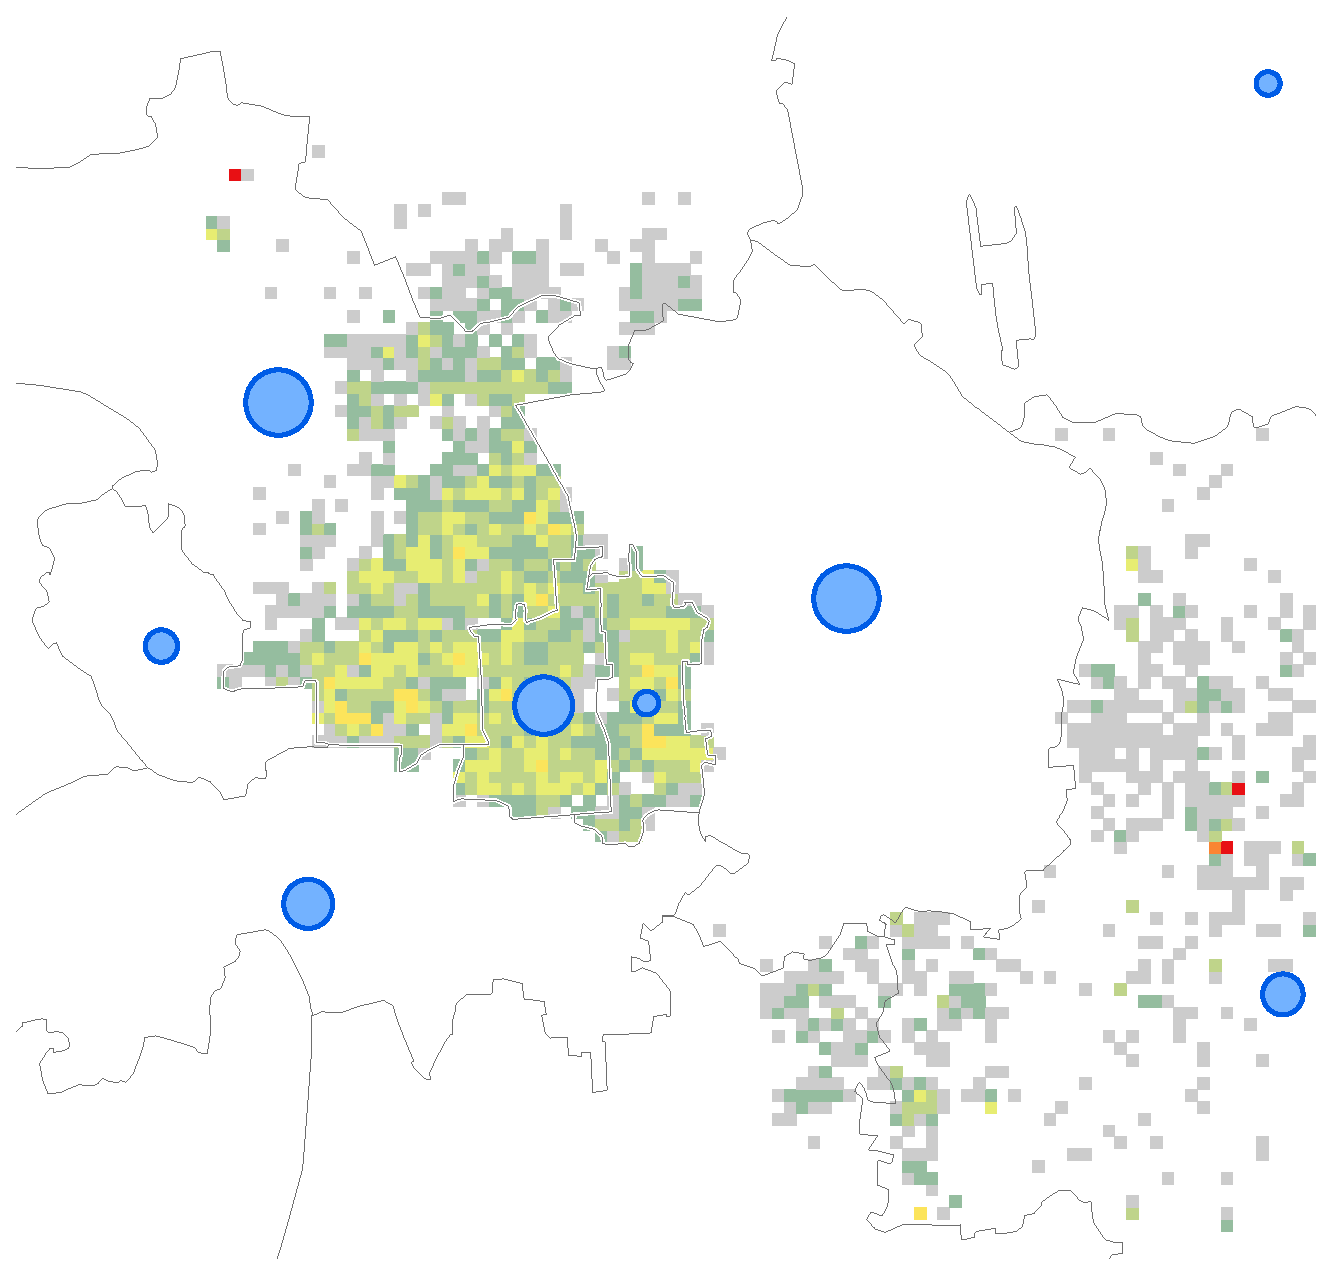
\includegraphics[width=\textwidth]{Figures/Relation_with_confrimed_cases/NewDistrictSSBD2020_02_08.eps}
        \caption{08 Feb}
    \end{subfigure}
    \begin{subfigure}{.3\textwidth}
        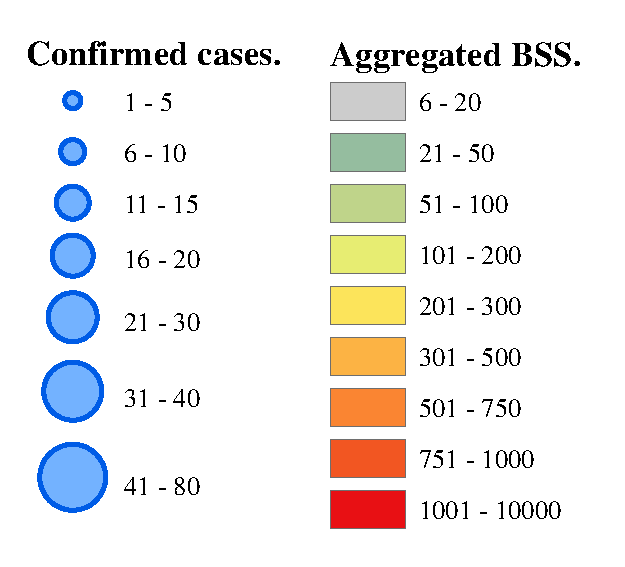
\includegraphics[width=\textwidth]{Figures/Relation_with_confrimed_cases/legend7.eps}
        \caption{legend}
    \end{subfigure}
    \caption{Relationships between cycling activities and confirmed cases during the quarantine period.}
    \label{fig:BSS_phase1_2}
\end{figure}
\textcolor{red}{After the epidemic is effectively controlled, cycling activities increased due to the rework requirements, which can be inferred from visual interpretation. The difference is obvious comparing workday and weekend.}
\begin{figure}[H]
    \centering
    \begin{subfigure}{.3\textwidth}
        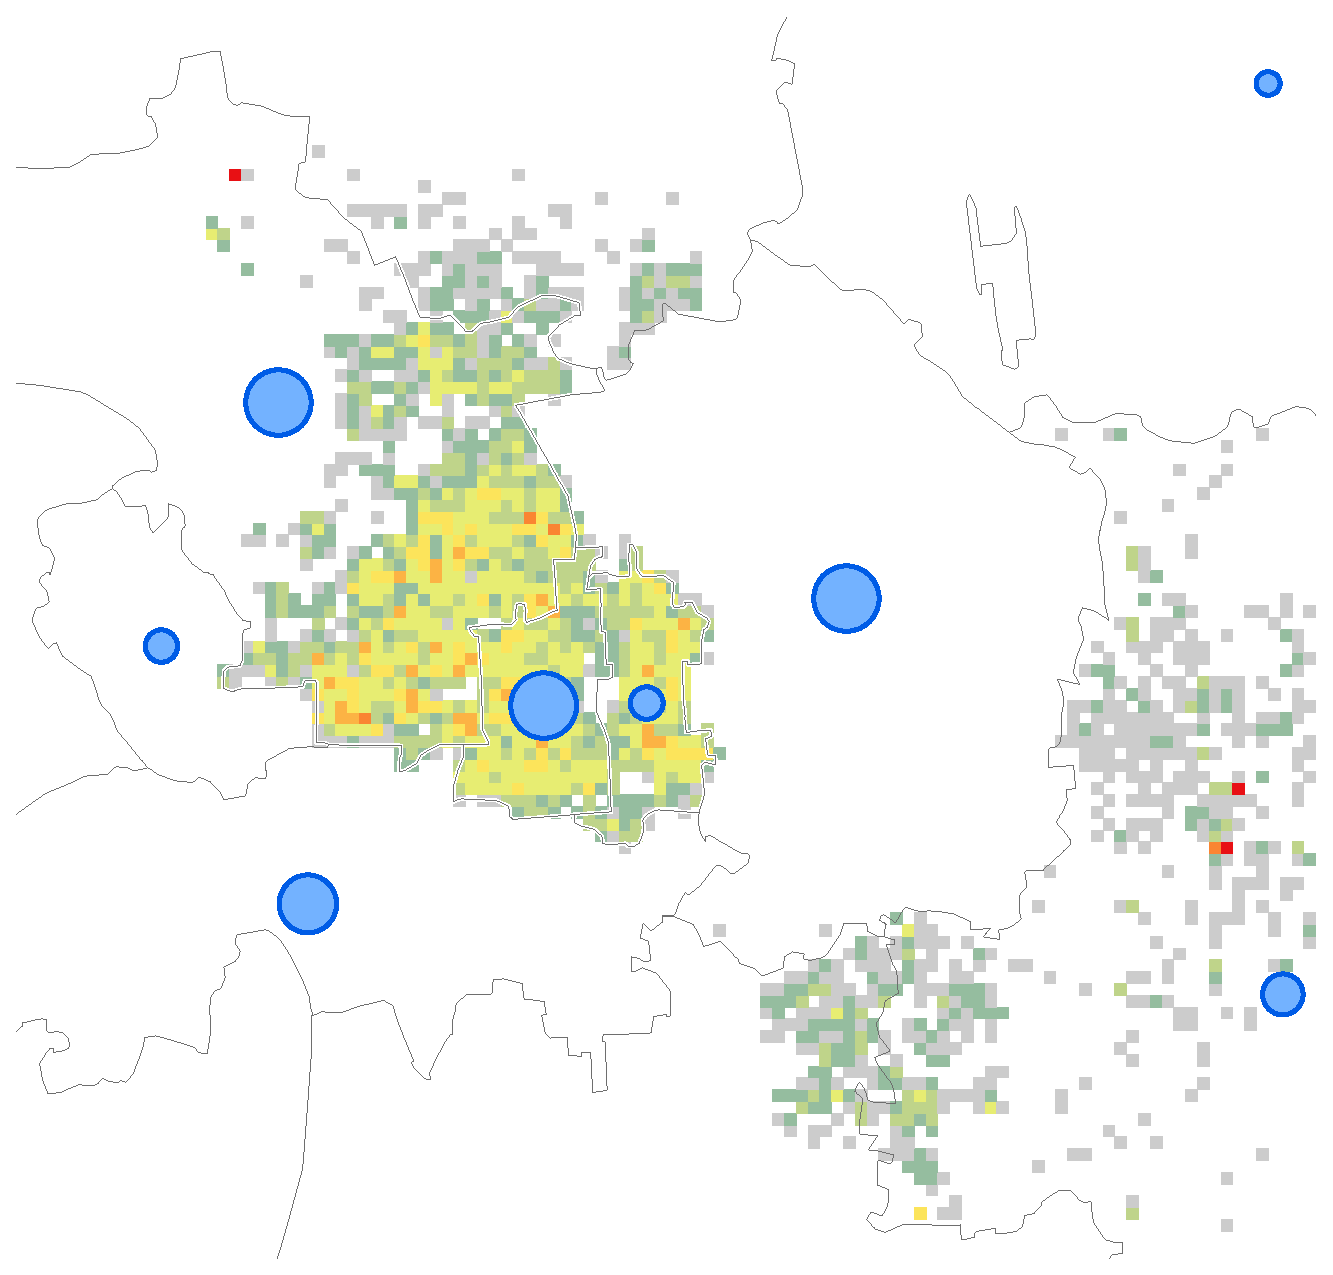
\includegraphics[width=\textwidth]{Figures/Relation_with_confrimed_cases/NewDistrictSSBD2020_02_12.eps}
        \caption{12 Feb}
    \end{subfigure}
    \begin{subfigure}{.3\textwidth}
        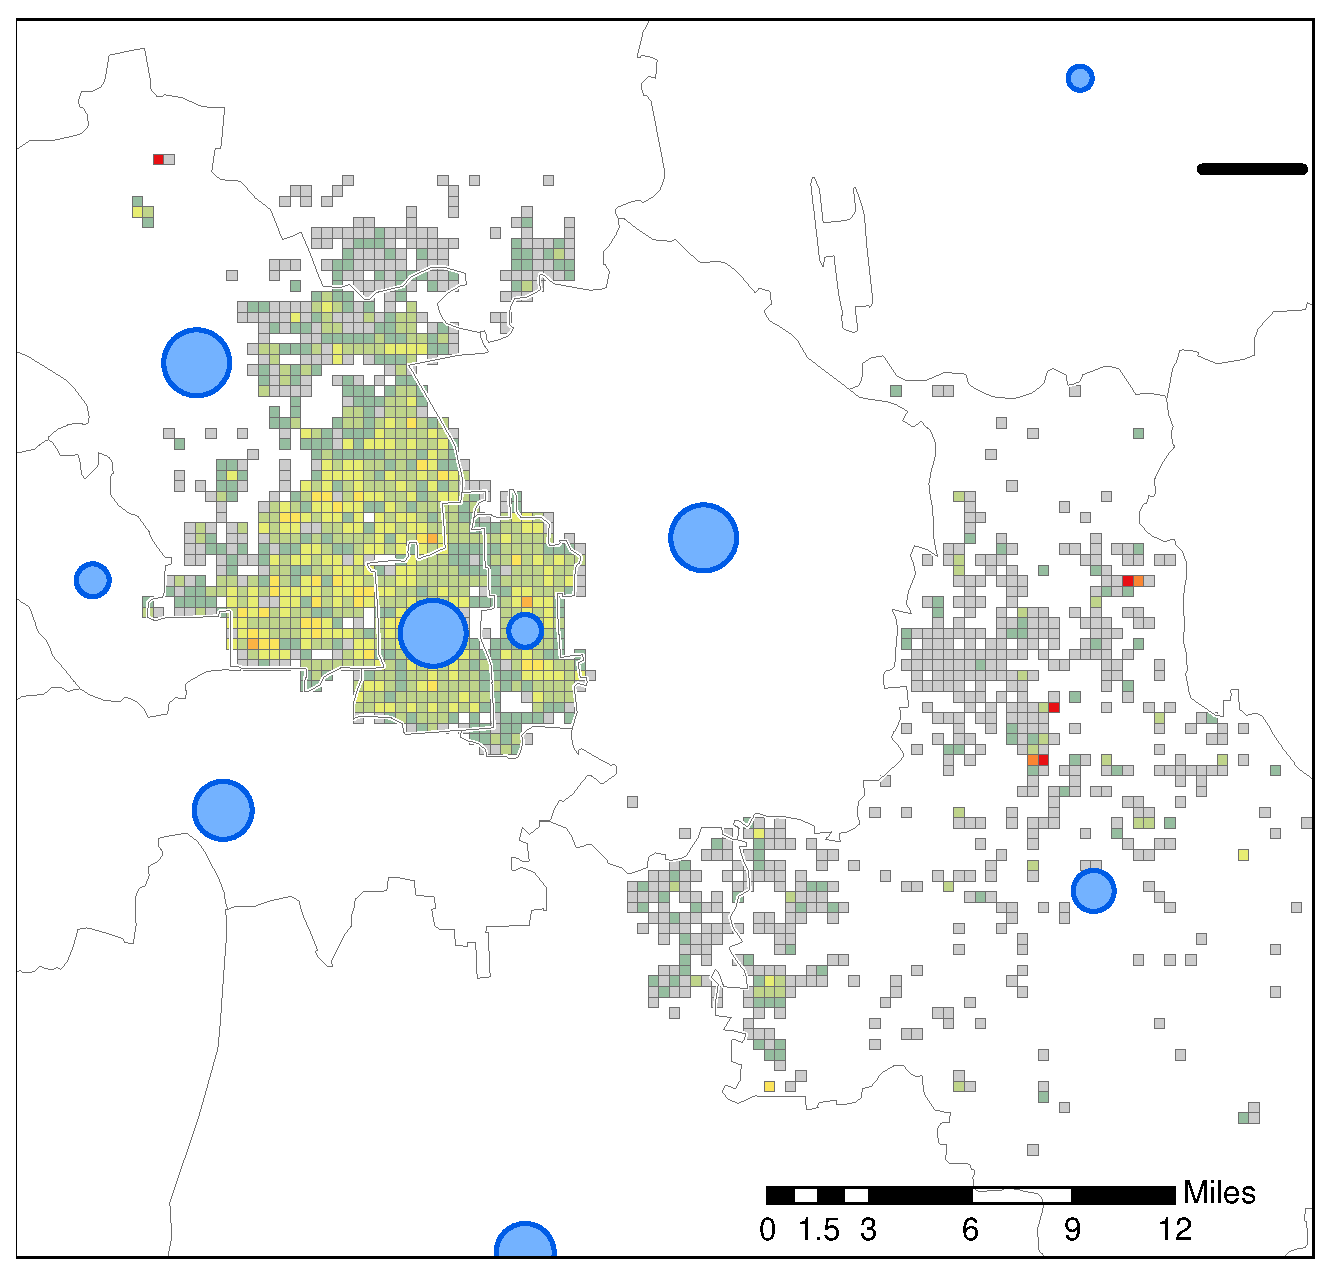
\includegraphics[width=\textwidth]{Figures/Relation_with_confrimed_cases/NewDistrictSSBD2020_02_16.eps}
        \caption{16 Feb}
    \end{subfigure}
    \begin{subfigure}{.3\textwidth}
        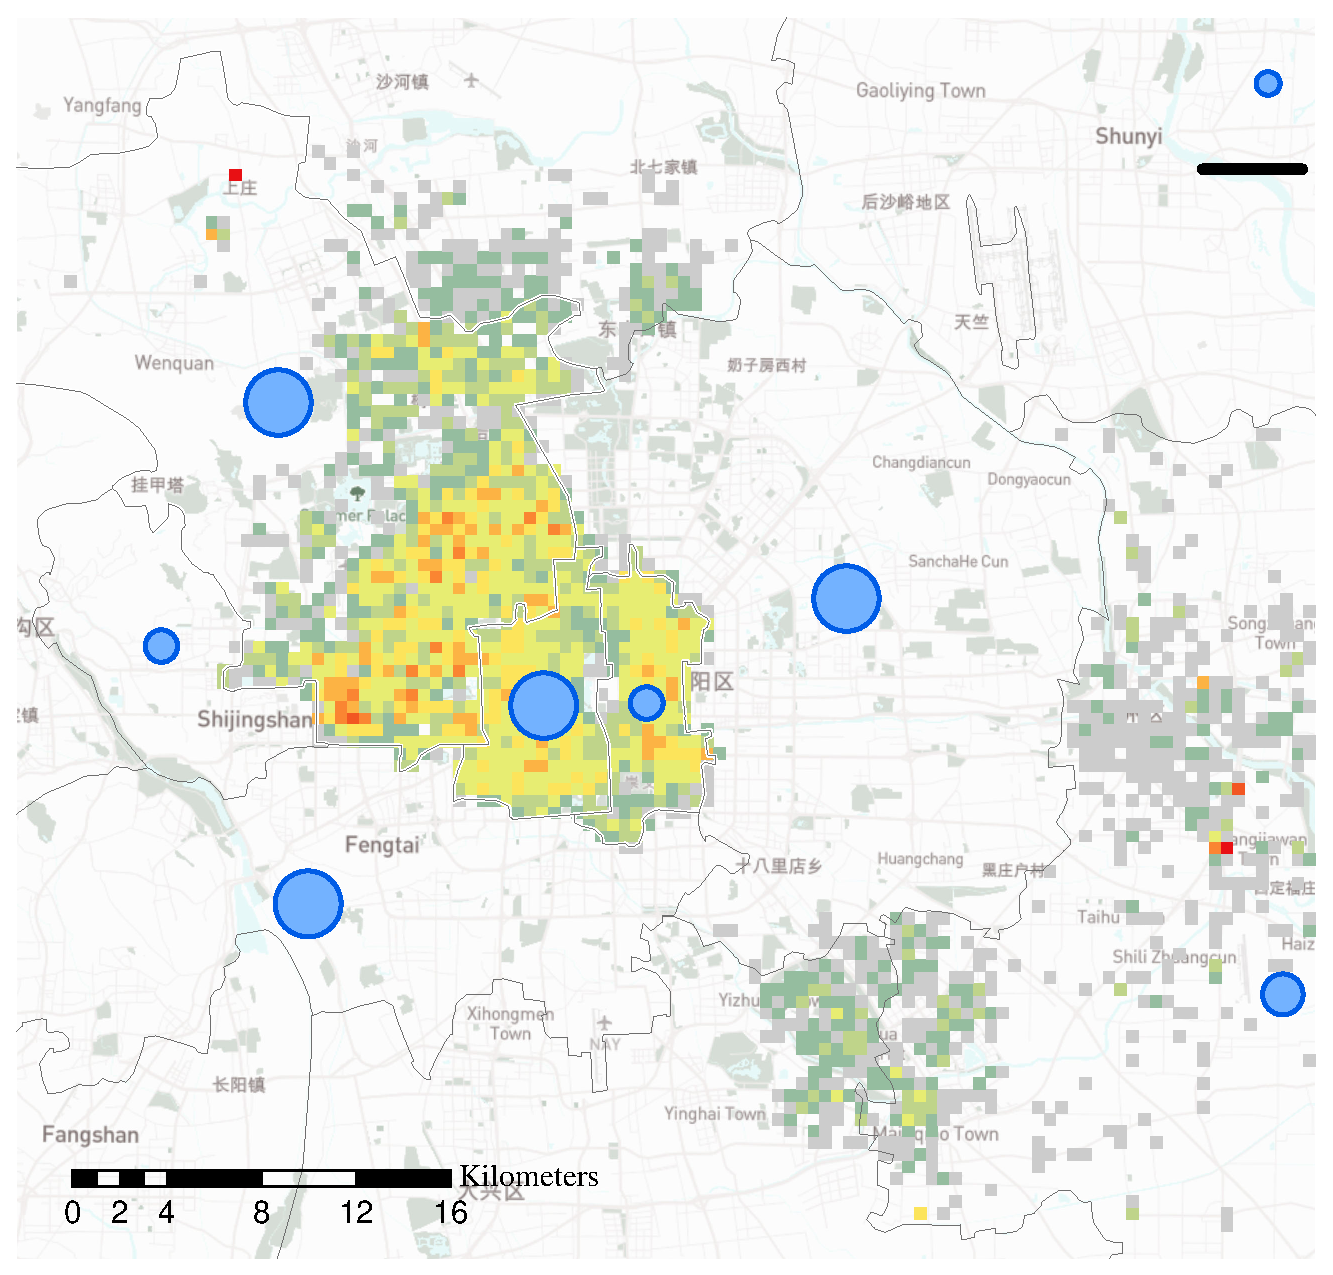
\includegraphics[width=\textwidth]{Figures/Relation_with_confrimed_cases/NewDistrictSSBD2020_02_20.eps}
        \caption{20 Feb}
    \end{subfigure}
    
    \vspace{6pt}
    \begin{subfigure}{.3\textwidth}
        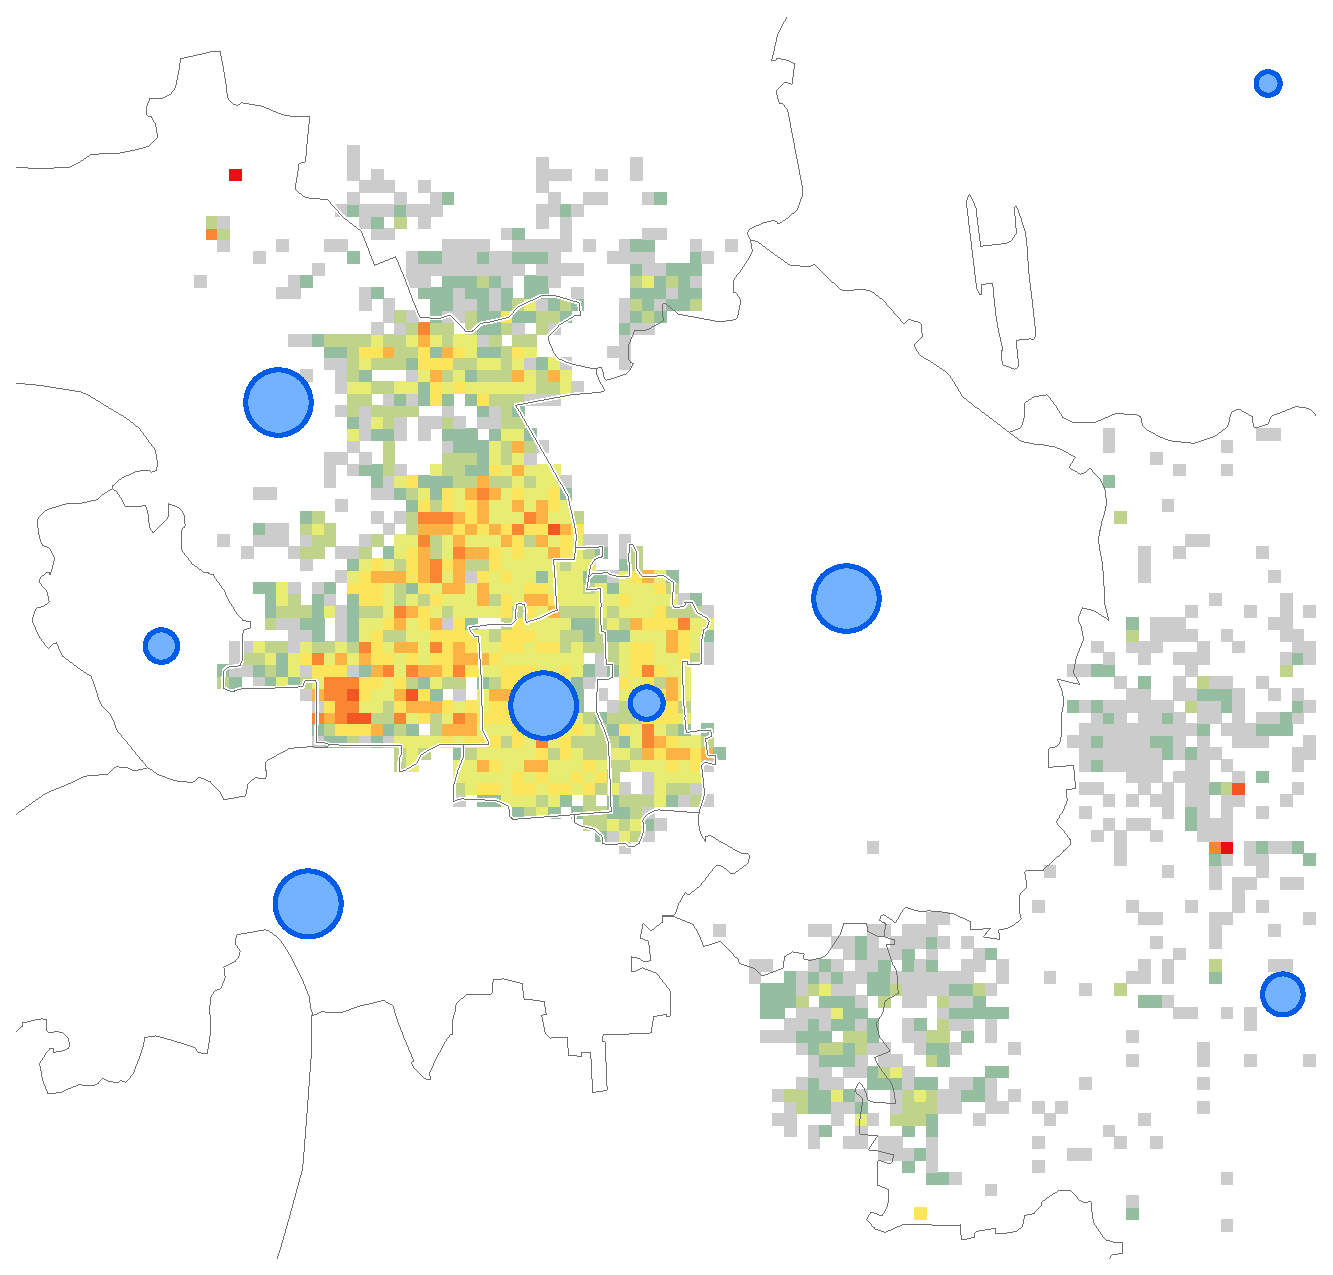
\includegraphics[width=\textwidth]{Figures/Relation_with_confrimed_cases/NewDistrictSSBD2020_02_24.eps}
        \caption{24 Feb}
    \end{subfigure}
    \begin{subfigure}{.3\textwidth}
        \includegraphics[width=\textwidth]{Figures/Relation_with_confrimed_cases/NewDistrictSSBD2020_02_28.eps}
        \caption{28 Feb}
    \end{subfigure}
    \begin{subfigure}{.3\textwidth}
        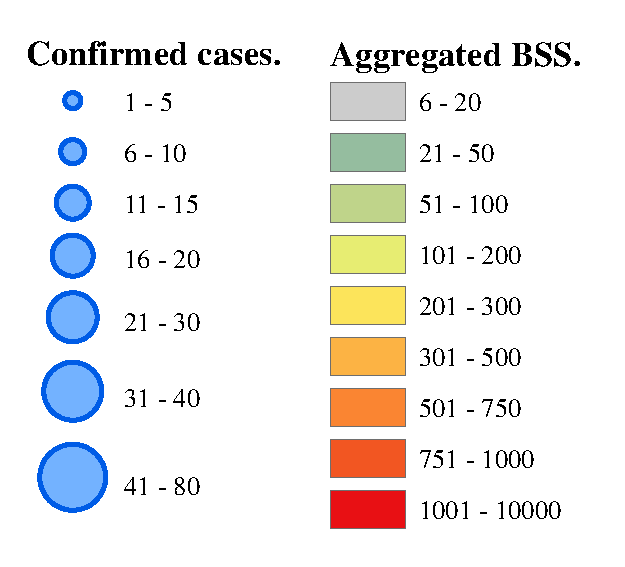
\includegraphics[width=\textwidth]{Figures/Relation_with_confrimed_cases/legend7.eps}
        \caption{legend}
    \end{subfigure}
    \caption{Relationships between cycling activities and confirmed cases when the epidemic is mitigated.}
    \label{fig:BSS_phase_3}
\end{figure}

\textit{Here insert Regression or correlation between them.}

%%%%%%%%%%%%%%%%%%%%%%%%%%%%%%%%%%%%%%%%%%%%%%
Part 3. Relationships between cycling activities and POIs
\textcolor{red}{Visual interpretation and analysis on communities and BSS usage with respect to epidemic period.}
\begin{figure}[H]
    \centering
    \begin{subfigure}{.23\textwidth}
        \includegraphics[width=\textwidth]{Figures/Relation_with_POIs/POI_resD2020_01_25.eps}
        \caption{25 Jan}
    \end{subfigure}
    \begin{subfigure}{.23\textwidth}
        \includegraphics[width=\textwidth]{Figures/Relation_with_POIs/POI_resD2020_02_09.eps}
        \caption{09 Feb}
    \end{subfigure}
    \begin{subfigure}{.23\textwidth}
        \includegraphics[width=\textwidth]{Figures/Relation_with_POIs/POI_resD2020_02_18.eps}
        \caption{18 Feb}
    \end{subfigure}
        \begin{subfigure}{.23\textwidth}
        \includegraphics[width=\textwidth]{Figures/Relation_with_POIs/POI_resD2020_03_02.eps}
        \caption{02 Mar}
    \end{subfigure}
    \caption{BSS and communities.}
    \label{fig:BSS_communities}
\end{figure}

\textcolor{red}{Visual interpretation and analysis on traffic/metro and BSS usage with respect to epidemic period.}
\begin{figure}[H]
    \centering
    \begin{subfigure}{.23\textwidth}
        \includegraphics[width=\textwidth]{Figures/Relation_with_POIs/POI_metroD2020_01_25.eps}
        \caption{25 Jan}
    \end{subfigure}
    \begin{subfigure}{.23\textwidth}
        \includegraphics[width=\textwidth]{Figures/Relation_with_POIs/POI_metroD2020_02_09.eps}
        \caption{09 Feb}
    \end{subfigure}
    \begin{subfigure}{.23\textwidth}
        \includegraphics[width=\textwidth]{Figures/Relation_with_POIs/POI_metroD2020_02_18.eps}
        \caption{18 Feb}
    \end{subfigure}
        \begin{subfigure}{.23\textwidth}
        \includegraphics[width=\textwidth]{Figures/Relation_with_POIs/POI_metroD2020_03_02.eps}
        \caption{02 Mar}
    \end{subfigure}
    \caption{BSS and metro.}
    \label{fig:BSS_metro}
\end{figure}

\textcolor{red}{Visual interpretation and analysis on malls and BSS usage with respect to epidemic period.}
\begin{figure}[H]
    \centering
    \begin{subfigure}{.23\textwidth}
        \includegraphics[width=\textwidth]{Figures/Relation_with_POIs/POI_mallsD2020_01_25.eps}
        \caption{25 Jan}
    \end{subfigure}
    \begin{subfigure}{.23\textwidth}
        \includegraphics[width=\textwidth]{Figures/Relation_with_POIs/POI_mallsD2020_02_09.eps}
        \caption{09 Feb}
    \end{subfigure}
    \begin{subfigure}{.23\textwidth}
        \includegraphics[width=\textwidth]{Figures/Relation_with_POIs/POI_mallsD2020_02_18.eps}
        \caption{18 Feb}
    \end{subfigure}
        \begin{subfigure}{.23\textwidth}
        \includegraphics[width=\textwidth]{Figures/Relation_with_POIs/POI_mallsD2020_03_02.eps}
        \caption{02 Mar}
    \end{subfigure}
    \caption{BSS and malls.}
    \label{fig:BSS_malls}
\end{figure}

\textcolor{red}{Visual interpretation and analysis on companies and BSS usage with respect to epidemic period.}
\begin{figure}[H]
    \centering
    \begin{subfigure}{.23\textwidth}
        \includegraphics[width=\textwidth]{Figures/Relation_with_POIs/POI_compD2020_01_25.eps}
        \caption{25 Jan}
    \end{subfigure}
    \begin{subfigure}{.23\textwidth}
        \includegraphics[width=\textwidth]{Figures/Relation_with_POIs/POI_compD2020_02_09.eps}
        \caption{09 Feb}
    \end{subfigure}
    \begin{subfigure}{.23\textwidth}
        \includegraphics[width=\textwidth]{Figures/Relation_with_POIs/POI_compD2020_02_18.eps}
        \caption{18 Feb}
    \end{subfigure}
        \begin{subfigure}{.23\textwidth}
        \includegraphics[width=\textwidth]{Figures/Relation_with_POIs/POI_compD2020_03_02.eps}
        \caption{02 Mar}
    \end{subfigure}
    \caption{BSS and companies.}
    \label{fig:BSS_companies}
\end{figure}

By removing the factor of Chinese new year, we observe a steep fall of overall share bike usage from 22 January to 29 Feb.
Industrial: IT,...
Residential: ...


\section{Conclusion}


%%%%%%%%%%%%%%%%%%%%%%%%%%%%%%%%%%%%%%%%%%
\vspace{6pt} 

%%%%%%%%%%%%%%%%%%%%%%%%%%%%%%%%%%%%%%%%%%
%% optional
%\supplementary{The following are available online at \linksupplementary{s1}, Figure S1: title, Table S1: title, Video S1: title.}

%%%%%%%%%%%%%%%%%%%%%%%%%%%%%%%%%%%%%%%%%%
%% optional
\abbreviations{The following abbreviations are used in this manuscript:

\noindent 
\begin{tabular}{@{}ll}
GIS & Geographic Information System \\
BSS & Bike Sharing System\\
POI & Point Of Interest

\end{tabular}}

%%%%%%%%%%%%%%%%%%%%%%%%%%%%%%%%%%%%%%%%%%
%% optional
\appendixtitles{no} %Leave argument "no" if all appendix headings stay EMPTY (then no dot is printed after "Appendix A"). If the appendix sections contain a heading then change the argument to "yes".
\appendix
\section{}
\unskip
\subsection{}

%%%%%%%%%%%%%%%%%%%%%%%%%%%%%%%%%%%%%%%%%%

\reftitle{References}

\externalbibliography{yes}
\bibliography{bib}

%%%%%%%%%%%%%%%%%%%%%%%%%%%%%%%%%%%%%%%%%%
%% optional
% \sampleavailability{Samples of the compounds ...... are available from the authors.}

%% for journal Sci
%\reviewreports{\\
%Reviewer 1 comments and authors’ response\\
%Reviewer 2 comments and authors’ response\\
%Reviewer 3 comments and authors’ response
%}

%%%%%%%%%%%%%%%%%%%%%%%%%%%%%%%%%%%%%%%%%%
\end{document}

